%%%%%%%%%%%%%%%%%%%%%%%%%%%%%%%%%%%%%%%%%%%%%%%%%%%%%%%%%%%%%%%%%%%%%%
%%  disstemplate.tex, to be compiled with latex.		     %
%%  08 April 2002	Version 4				     %
%%%%%%%%%%%%%%%%%%%%%%%%%%%%%%%%%%%%%%%%%%%%%%%%%%%%%%%%%%%%%%%%%%%%%%
%%								     %
%%  Writing a Doctoral Dissertation with LaTeX at		     %
%%	the University of Texas at Austin			     %
%%								     %
%%  (Modify this ``template'' for your own dissertation.)	     %
%%								     %
%%%%%%%%%%%%%%%%%%%%%%%%%%%%%%%%%%%%%%%%%%%%%%%%%%%%%%%%%%%%%%%%%%%%%%


\documentclass[12pt]{report}	% The documentclass must be ``report''.

\usepackage{utdiss2-05}  		% Dissertation package style file.


%%%%%%%%%%%%%%%%%%%%%%%%%%%%%%%%%%%%%%%%%%%%%%%%%%%%%%%%%%%%%%%%%%%%%%
% Optional packages used for this sample dissertation. If you don't  %
% need a capability in your dissertation, feel free to comment out   %
% the package usage command.					     %
%%%%%%%%%%%%%%%%%%%%%%%%%%%%%%%%%%%%%%%%%%%%%%%%%%%%%%%%%%%%%%%%%%%%%%

\usepackage{amsmath,amsthm,amsfonts,amscd} 
				% Some packages to write mathematics.
\usepackage{eucal} 	 	% Euler fonts
\usepackage{verbatim}      	% Allows quoting source with commands.
\usepackage{makeidx}       	% Package to make an index.
\usepackage{graphicx}
\usepackage{siunitx}
\usepackage{float}
\usepackage{tikz}		%Graphics package
\usepackage{schemabloc} 	%Block Diagram package
\usepackage[american, arrowmos]{circuitikz}	%Circuit optimized graphics package
\usepackage{epstopdf}	%Included epstopdf for inclusion of eps files in pdfLaTeX
\usepackage{epsfig}         	% Allows inclusion of eps files.
%\usepackage{citesort}         	% 
\usepackage{url}		% Allows good typesetting of web URLs.
\usepackage{xfrac}
\usepackage{nicefrac}
\usepackage{chngpage}
\usepackage{tabularx}
\usepackage{fixltx2e}
%\usepackage{draftcopy}		% Uncomment this line to have the
				% word, "DRAFT," as a background
				% "watermark" on all of the pages of
				% of your draft versions. When ready
				% to generate your final copy, re-comment
				% it out with a percent sign to remove
				% the word draft before you re-run
				% Makediss for the last time.

\usetikzlibrary{circuits}
\usetikzlibrary{shapes,arrows}
\author{Miguel Francisco Gandara}  	% Required

\address{1023 Cragmore Dr.\\ Seabrook, TX 77586}  % Required

\title{A 12-bit, 10 Msps Two Stage SAR-Based Pipeline ADC}
                                                    % Required

%%%%%%%%%%%%%%%%%%%%%%%%%%%%%%%%%%%%%%%%%%%%%%%%%%%%%%%%%%%%%%%%%%%%%%
% NOTICE: The total number of supervisors and other members %%%%%%%%%%
%%%%%%%%%%%%%%% MUST be seven (7) or less! If you put in more, %%%%%%%
%%%%%%%%%%%%%%% they are put on the page after the Committee %%%%%%%%%
%%%%%%%%%%%%%%% Certification of Approved Version page. %%%%%%%%%%%%%%
%%%%%%%%%%%%%%%%%%%%%%%%%%%%%%%%%%%%%%%%%%%%%%%%%%%%%%%%%%%%%%%%%%%%%%

%%%%%%%%%%%%%%%%%%%%%%%%%%%%%%%%%%%%%%%%%%%%%%%%%%%%%%%%%%%%%%%%%%%%%%
%
% Enter names of the supervisor and co-supervisor(s), if any,
% of your dissertation committee. Put one name per line with
% the name in square brackets. The name on the last line, however,
% must be in curly braces.
%
% If you have only one supervisor, the entry below will read:
%
%	\supervisor
%		{Supervisor's Name}
%
% NOTE: Maximum three supervisors. Minimum one supervisor.
% NOTE: The Office of Graduate Studies will accept only two supervisors!
% 
%
\supervisor
	{Nan Sun}

%%%%%%%%%%%%%%%%%%%%%%%%%%%%%%%%%%%%%%%%%%%%%%%%%%%%%%%%%%%%%%%%%%%%%%
%
% Enter names of the other (non-supervisor) members(s) of your
% dissertation committee. Put one name per line with the name
% in square brackets. The name on the last line, however, must
% be in curly braces.
%
% NOTE: Maximum six other members. Minimum zero other members.
% NOTE: The Office of Graduate Studies may restrict you to a total
%	of six committee members.
%
%
\committeemembers
	{Ranjit Gharpurey}

%%%%%%%%%%%%%%%%%%%%%%%%%%%%%%%%%%%%%%%%%%%%%%%%%%%%%%%%%%%%%%%%%%%%%%

\previousdegrees{B.S.E.E.}
     % The abbreviated form of your previous degree(s).
     % E.g., \previousdegrees{B.S., MBA}.
     %
     % The default value is `B.S., M.S.'

\graduationmonth{December}      
     % Graduation month, either May, August, or December, in the form
     % as `\graduationmonth{May}'. Do not abbreviate.
     %
     % The default value (either May, August, or December) is guessed
     % according to the time of running LaTeX.

\graduationyear{2012}   
     % Graduation year, in the form as `\graduationyear{2001}'.
     % Use a 4 digit (not a 2 digit) number.
     %
     % The default value is guessed according to the time of 
     % running LaTeX.

%\typist{...}       
     % The name(s) of typist(s), put `the author' if you do it yourself.
     % E.g., `\typist{Maryann Hersey and the author}'.
     %
     % The default value is `the author'.


%%%%%%%%%%%%%%%%%%%%%%%%%%%%%%%%%%%%%%%%%%%%%%%%%%%%%%%%%%%%%%%%%%%%%%
% Commands for master's theses and reports.			     %
%%%%%%%%%%%%%%%%%%%%%%%%%%%%%%%%%%%%%%%%%%%%%%%%%%%%%%%%%%%%%%%%%%%%%%
%
% If the degree you're seeking is NOT Doctor of Philosophy, uncomment
% (remove the % in front of) the following two command lines (the ones
% that have the \ as their second character).
%
\degree{Master of Science in Engineering}
\degreeabbr{M.S.E.}

% Uncomment the line below that corresponds to the type of master's
% document you are writing.
%
\masterreport
%\masterthesis


%%%%%%%%%%%%%%%%%%%%%%%%%%%%%%%%%%%%%%%%%%%%%%%%%%%%%%%%%%%%%%%%%%%%%%
% Some optional commands to change the document's defaults.	     %
%%%%%%%%%%%%%%%%%%%%%%%%%%%%%%%%%%%%%%%%%%%%%%%%%%%%%%%%%%%%%%%%%%%%%%
%
%\singlespacing
%\oneandonehalfspacing

%\singlespacequote
\oneandonehalfspacequote

\topmargin 0.125in	% Adjust this value if the PostScript file output
			% of your dissertation has incorrect top and 
			% bottom margins. Print a copy of at least one
			% full page of your dissertation (not the first
			% page of a chapter) and measure the top and
			% bottom margins with a ruler. You must have
			% a top margin of 1.5" and a bottom margin of
			% at least 1.25". The page numbers must be at
			% least 1.00" from the bottom of the page.
			% If the margins are not correct, adjust this
			% value accordingly and re-compile and print again.
			%
			% The default value is 0.125"

		% If you want to adjust other margins, they are in the
		% utdiss2-nn.sty file near the top. If you are using
		% the shell script Makediss on a Unix/Linux system, make
		% your changes in the utdiss2-nn.sty file instead of
		% utdiss2.sty because Makediss will overwrite any changes
		% made to utdiss2.sty.

%%%%%%%%%%%%%%%%%%%%%%%%%%%%%%%%%%%%%%%%%%%%%%%%%%%%%%%%%%%%%%%%%%%%%%
% Some optional commands to be tested.				     %
%%%%%%%%%%%%%%%%%%%%%%%%%%%%%%%%%%%%%%%%%%%%%%%%%%%%%%%%%%%%%%%%%%%%%%

% If there are 10 or more sections, 10 or more subsections for a section,
% etc., you need to make an adjustment to the Table of Contents with the
% command \longtocentry.
%
%\longtocentry 



%%%%%%%%%%%%%%%%%%%%%%%%%%%%%%%%%%%%%%%%%%%%%%%%%%%%%%%%%%%%%%%%%%%%%%
%	Some math support.					     %
%%%%%%%%%%%%%%%%%%%%%%%%%%%%%%%%%%%%%%%%%%%%%%%%%%%%%%%%%%%%%%%%%%%%%%
%
%	Theorem environments (these need the amsthm package)
%
%% \theoremstyle{plain} %% This is the default

\newtheorem{thm}{Theorem}[section]
\newtheorem{cor}[thm]{Corollary}
\newtheorem{lem}[thm]{Lemma}
\newtheorem{prop}[thm]{Proposition}
\newtheorem{ax}{Axiom}

\theoremstyle{definition}
\newtheorem{defn}{Definition}[section]

\theoremstyle{remark}
\newtheorem{rem}{Remark}[section]
\newtheorem*{notation}{Notation}

%\numberwithin{equation}{section}


%%%%%%%%%%%%%%%%%%%%%%%%%%%%%%%%%%%%%%%%%%%%%%%%%%%%%%%%%%%%%%%%%%%%%%
%	Macros.							     %
%%%%%%%%%%%%%%%%%%%%%%%%%%%%%%%%%%%%%%%%%%%%%%%%%%%%%%%%%%%%%%%%%%%%%%
%
%	Here some macros that are needed in this document:


\newcommand{\latexe}{{\LaTeX\kern.125em2%
                      \lower.5ex\hbox{$\varepsilon$}}}

\newcommand{\amslatex}{\AmS-\LaTeX{}}
\newcommand{\gmid}{$g_m/I_{d}$}
\newcommand{\gmgds}{$g_m/g_{ds}$}
\newcommand{\gmro}{$g_mr_o$}
\newcommand{\transit}{$\omega_{T}$}
\newcommand{\spc}{\mbox{ }}
\newcommand{\ff}{\si{\femto\farad}}
\newcommand{\pf}{\si{\pico\farad}}
\newcommand{\nonu}{\nonumber}
\newcommand{\csone}{$C_{s1}$}
\newcommand{\cstwo}{$C_{s2}$}
\newcommand{\cf}{$C_{f}$}
\newcommand{\tnot}{$T_{0}$}
\newcommand{\ed}{$\epsilon_{d}$}
\newcommand{\es}{$\epsilon_{s}$}
\newcommand{\Gm}{$G_{m}$}
\newcommand{\Ro}{$R_{o}$}
\newcommand{\aoldc}{$A_{OLDC}$}
\newcommand{\Gain}{\emph{Gain}}

\chardef\bslash=`\\	% \bslash makes a backslash (in tt fonts)
			%	p. 424, TeXbook

\newcommand{\cn}[1]{\texttt{\bslash #1}}

\makeatletter		% Starts section where @ is considered a letter
			% and thus may be used in commands.
\def\square{\RIfM@\bgroup\else$\bgroup\aftergroup$\fi
  \vcenter{\hrule\hbox{\vrule\@height.6em\kern.6em\vrule}%
                                              \hrule}\egroup}
\makeatother		% Ends sections where @ is considered a letter.
			% Now @ cannot be used in commands.

%\makeindex    % Make the index

%%%%%%%%%%%%%%%%%%%%%%%%%%%%%%%%%%%%%%%%%%%%%%%%%%%%%%%%%%%%%%%%%%%%%%
%		The document starts here.			     %
%%%%%%%%%%%%%%%%%%%%%%%%%%%%%%%%%%%%%%%%%%%%%%%%%%%%%%%%%%%%%%%%%%%%%%

\begin{document}

\copyrightpage          % Produces the copyright page.


%
% NOTE: In a doctoral dissertation, the Committee Certification page
%		(with signatures) is BEFORE the Title page.
%	In a masters thesis or report, the Signature page
%		(with signatures) is AFTER the Title page.
%
%	If you are writing a masters thesis or report, you MUST REVERSE
%	the order of the \commcertpage and \titlepage commands below.
%
\commcertpage           % Produces the Committee Certification
			%   of Approved Version page (doctoral)
			%   or Signature page (masters).
			%		20 Mar 2002	cwm

\titlepage              % Produces the title page.







%%%%%%%%%%%%%%%%%%%%%%%%%%%%%%%%%%%%%%%%%%%%%%%%%%%%%%%%%%%%%%%%%%%%%%
% Dedication and/or epigraph are optional, but must occur here.      %
%%%%%%%%%%%%%%%%%%%%%%%%%%%%%%%%%%%%%%%%%%%%%%%%%%%%%%%%%%%%%%%%%%%%%%
%
\begin{dedication}
%\index{Dedication@\emph{Dedication}}%
Dedicated to God and to my family.
\end{dedication}


\begin{acknowledgments}		% Optional
%\index{Acknowledgments@\emph{Acknowledgments}}%
I would like to thank my supervisor Professor Nan Sun for all of his advice, encouragement, and for always pushing me to deliver excellent work. I would also like to thank Professor Ranjit Gharpurey for agreeing to be the reader for this report and making his analog classes interesting. I would also like to thank Professor Deji Akinwande for sparking my interest in analog circuit design in my first semester of graduate school.

This work would not have been possible without all the love and support I received from my family: my parents Miguel and Kathryn, my stepdad Jeremy, my siblings Julia, Liam, and Emma, and the love of my life, Disha. Their support throughout my graduate career pushed me to produce my best work and carried me through many stressful times. I cannot thank each of these people enough.

Finally, I would like to thank all of my classmates. This experience would not have been nearly as rewarding or fun without our late nights of struggling through homework and labs.
\end{acknowledgments}


% The abstract is required. Note the use of ``utabstract'' instead of
% ``abstract''! This was necessary to fix a page numbering problem.
% The abstract heading is generated automatically.
% Do NOT use \begin{abstract} ... \end{abstract}.
%
\utabstract

The market for battery powered communications devices has grown significantly in recent years. These devices require a large number of analog to digital converters (ADCs) to transform wireless and other physical data into the digital signals required for digital signal processing elements and microprocessors. For these applications, power efficiency and accuracy are of the utmost importance. Successive approximation register (SAR) ADCs are frequently used in power constrained applications, but their main limitation is their low sampling rate. In this work, a two stage pipelined ADC is presented that attempts to mitigate some of the sampling rate limitations of a SAR while maintaining its power and resolution advantages. Special techniques are used to reduce the overall sampling capacitance required in both SAR stages and to increase the linearity of the multiplying digital to analog converter (MDAC) output. The SAR sampling network, control logic, and MDAC  blocks are completely implemented. Ideal components were used for the clocking, comparators, and switches. At the end of this design, a figure of merit of \SI{51}{\femto\joule}/conversion-step was achieved.
\index{Abstract}%
\indent

\tableofcontents   % Table of Contents will be automatically
                   % generated and placed here.

\listoftables      % List of Tables and List of Figures will be placed
\listoffigures     % here, if applicable.



%%%%%%%%%%%%%%%%%%%%%%%%%%%%%%%%%%%%%%%%%%%%%%%%%%%%%%%%%%%%%%%%%%%%%%
% Actual text starts here.					     %
%%%%%%%%%%%%%%%%%%%%%%%%%%%%%%%%%%%%%%%%%%%%%%%%%%%%%%%%%%%%%%%%%%%%%%
%
% Including external files for each chapter makes this document simpler,
% makes each chapter simpler, and allows for generating test documents
% with as few as zero chapters (by commenting out the include statements).
% This allows quicker processing by the Makediss command file in case you
% are not working on a specific, long and slow to compile chapter. You
% can even change the chapter order by merely interchanging the order
% of the include statements (something I found helpful in my own
% dissertation).
%
\tikzstyle{block} = [draw, rectangle, minimum height=2em]
\tikzstyle{sum} = [draw, circle, node distance=1cm]
\tikzstyle{input} = [coordinate]
\tikzstyle{output} = [coordinate]
\tikzstyle{pinstyle} = [pin edge={to-,thin,black}]
\tikzstyle{amp} = [draw, isosceles triangle, node distance=1cm]
\chapter{Introduction}
\label{chap:introduction}
The movement to smart mobile connected devices which consolidate functions of traditionally separate devices is driving innovation in System-on-chips (SoCs).  One of the innovations helping to meet the current needs of SoCs is the integration of larger memory with the processor.  As the need for memory has increased, SoCs have moved from logic dominant chips to memory dominant chips.  In fact, \cite{1327984} estimates 94\% of the SoC will be dedicated to memory by 2014.  

Because embedded memories are designed with aggressive design rules to increase the density of transistors per area, they are more prone to manufacturing defects that negatively affect the overall chip yield.  Testing memory to identify faulty blocks is critical to increase and maintain acceptable yield \cite{1395663}. 
A built-in self-test (BIST) has previously been used to test logical elements of the chip, but now have been adapted to test memory as well.  The density of memory and difficulty in accessing all signals has driven the growth of memory built-in self-test (MBIST) as the only practical and cost-effect solution for embedded SoC memories \cite{5875994}.  

As not all fault models can always be predicted for a new product, programmable MBIST (PMBIST) designs allow developers to address fault detection, create efficient algorithms, and overcome challenges presented by new technology.  Conversely, a non-programmable MBIST requires the designer to correctly predict the fault models to be tested, but changes to the design or mask typically requires another tape-out and can be quite expensive.  Because of this, the programmable MBIST has gained popularity amongst memory designers. 

The most common memory test today is the March test because its structured and repetitive algorithms can be applied very easily to the symmetric nature of memory cells \cite{1675150}.  The design presented in \cite{1584083} primarily uses the March test to verify the integrity of the memory.  In general, there are three components of memory tests: the test algorithm or operations in each cell; the data; and the memory address sequence \cite{5993815}.  

The PMBIST design presented in \cite{1584083} will be used as the base design and is intended to provide an area efficient design with good flexibility on algorithm and test data programming.  This report proposes improvements to the design by providing programmability to the address order and counting method. The previous design uses a linear counter and pseudo-random counter to sequence through memory addresses.  This allows the BIST to run March algorithms, but another algorithm, Moving Inversion (MOVI) cannot be run because it requires 2\textsuperscript{i} address counting method.   MOVI is popular industry for its ability to detect read and write disturbance while also allowing for determination of the best and worst case memory access times \cite{VanDeGoor1991}.  This project adds the 2\textsuperscript{i} counting method along with Gray coding and Address Compliment to integrate common industry test addressing sequences into the BIST. 

In addition, this paper will show a reduction of area can be achieved by introducing a dynamic pattern generation block to replace the auxiliary memory used to store neighborhood pattern-sensitive fault (NPSF) backgrounds.  In the base design, the data pattern for auxiliary memory can initialized through a scan mechanism \cite{748806}, but relying solely on scan to load data patterns can be time consuming for serial BIST schemes.  Additionally, the MOVI fault model requires an NPSF data background of Type 1 to be effective.  Because of this, this report integrates an NPSF data background generator to remove the scan delay.  This provides faster access time and potentially removes the need for an auxiliary memory thus speeding up test time and saving area.  In achieving these design goals, this report will show enhancements to the \cite{1584083} design in two of the three memory test components.

This paper is divided into five chapters.
Chapter 1 offers motivation for this project and supplies definitions for common terminology.  Chapter 2 provides background information on the memory faults, current memory testing algorithms and designs to address some of the challenges of memory testing.  Chapter 3 presents details of the design proposed in this report and chapter 4 follows with testing results and comparisons to other designs.
Finally, chapter 5 concludes the report.  

\section{Memory BIST Terminology}
\label{sect:int-terminology}
BIST - Built-In Self-Test

MBIST - Memory BIST

PMBIST - Programmable MBIST

SoC - System-on-Chip

NPSF - Neighborhood Pattern-Sensitive Fault

ANPSF - Active NPSF

PNPSF - Passive NPSF

SAF - Stuck-At Fault

CF - Coupling Fault

TF - Transitional Fault




\chapter{Architectural Features}
Using the pipeline and SAR architectures described in Chapter \ref{chap:introduction}, some high-level architectural decisions had to be made, mainly relating to the partitioning of the design. In addition, some enhancements were applied to the basic architectures in order to enhance overall performance. These decisions and enhancements are the subject of this chapter.
\section{Architectural Decisions}
Before any block-level specifications could be created, the partitioning of the pipeline stages had to be decided. First the total number of pipeline stages needed to be decided. Next, the resolutions for each stage needed to be decided. Finally, a suitable redundancy scheme for design had to be chosen.
\subsection{Number of Pipeline Stages}
The discussion in Section \ref{sec:pipelinesaradv} highlights the diminishing returns of increasing the number of pipeline stages. Beyond two pipeline stages, the effect on power consumption from the reduction in capacitance 
would likely be outweighed by the power consumption of the additional MDAC OTA. Similarly, to realize the potential benefits of pipelining on the speed of the ADC, the speed of the comparator must be increased as well. At 
some point, this will place a prohibitive constraint on the comparator speed. In addition, SAR converters show the most advantage over flash ADC's at higher resolutions. Using more than two pipeline stage for a 12 bit design 
would require an average stage resolution of 3 or less bits. In addition, from the discussion in Section \ref{sec:highfirstres}, a high first stage resolution is desired to achieve maximum benefits. For these reasons, a two 
stage design was chosen.
\subsection{Operation Partitioning}
After determining the number of stages, each stage's required operations must be partitioned between the two phases of the sampling clock. For the second stage ADC, which must only perform sampling and conversion, partitioning the operations between the two clock phases is straightforward. Due to the latency introduced by the first stage, the sampling will occur in the second clock phase, and the conversion will occur in the first clock phase of the next clock cycle. The first stage ADC must perform three operations: sampling, conversion, and amplification. Assuming that half of a clock phase is allotted for conversion, this means that either the sampling or the conversion time must be halved. To achieve the same sampling resolution in half the time, the input switch resistance must be halved. Similarly, to achieve the same static error from the MDAC in half the time, the MDAC bandwidth must be doubled. Another side effect to sharing a clock phase between conversion and amplification is that the available sampling time for the second stage would also be halved. In general, reducing switch resistance is simpler to implement than increasing the MDAC bandwidth. In addition, doubling the MDAC bandwidth would likely increase power consumption more than halving the switch resistance. For these reasons, as well as the lack of side effects on the second stage, the sampling and conversion phases were combined in this design.
\subsection{Stage Resolution}
Next, the resolutions for each stage had to be determined. From the above discussion, the conversion time for the first stage will be half that of the second stage. From Equation \ref{eq:compdecisiontimegiventsamp}, for equivalent comparator specifications in both stages, the ratio of second stage resolution to first stage resolution should be 2:1. In a 12 bit ADC, this would mean a 4 bit first stage and an 8 bit second stage. While one may assume that the eight bit second stage would require a much larger DAC settling time, this would likely not be the case. A first stage resolution of 4 bits would imply a high closed loop gain in the MDAC. The high closed loop MDAC gain means that the input-referred offset noise of the second stage capacitor array is significantly reduced. This reduction in input-referred noise means that the unit capacitor for the second stage ADC could be decreased, and thus the difference between the capacitance of the two stages would likely not be significant. Beyond simply striving for equivalent comparator specifications, the first stage resolution should be as high as possible in order to achieve all the benefits from Section \ref{sec:highfirstres}. A fundamental limit to the benefits of first stage resolution does exist, however. This limit is due to the output parasitics in the MDAC OTA. From Equation \ref{eq:vres}, $G_m$ can be decreased in part because each 1-bit increase in first stage resolution decreases $C_{L,tot}$ by a factor of 2. This decrease in $C_{L,tot}$ no longer applies once the load capacitance becomes dominated by the self-parasitics of the MDAC op-amp. This implies that, for optimized power consumption, the first stage resolution should be increased to the point that output capacitance is dominated by the op-amp parasitics~\cite{5714725}. The issue with using the parasitics of the op-amp as the deciding factor for stage resolution is that without knowledge of stage resolution, the requirements for MDAC bandwidth and loop gain cannot be known. These specifications are strongly linked to parasitic capacitance size, and thus a sort of chicken and egg problem is created. In~\cite{5714725}, a 5 bit first stage and a 7 bit second stage were used, so this was used as a starting point. This also seemed like a reasonable partition in terms of comparator specifications. The speed requirement for the second stage comparator is relaxed with this partitioning, but this can also mean that a lower power comparator can theoretically be used for the second stage.
 \subsection{MDAC Redundancy Scheme}
 Without MDAC redundancy, overloading of the second stage ADC is basically guaranteed. For the purposes of this design, it was decided that 1 bit redundancy was the preferred scheme. First, the high stage resolution places stricter requirements on the comparator offset, so the additional offset headroom provided by 1-bit redundancy makes comparator implementation simpler. Second, unlike in flash ADCs, the implementation of a half bit of redundancy in SAR ADCs is not very straightforward. For flash ADCs, a half bit of redundancy involves the addition of comparators and the modification of their reference voltages. Implementing half bit redundancy in a SAR ADC would require changing the fundamental binary search algorithm used, which is a much more significant design modification. Implementing an extra bit of redundancy for a SAR, on the other hand, requires the addition of a single capacitor and an increase in comparator speed requirements. For these reasons, 1 bit redundancy was used. 
 \section{Architectural Enhancements}
 Beyond the basic pipeline and SAR architectures discussed in Sections \ref{sec:pipelineadcbasics} and \ref{sec:saradcbasics}, respectively, some additional architectural enhancements were used. First, a half-gain MDAC architecture was used. Second, the dummy LSB in the SAR sub-ADCs was exploited to achieve an additional bit of resolution.
 \subsection{Half-Gain MDAC}
 In~\cite{5714725}, an MDAC with a half-gain architecture is used to decrease power consumption. In general MDAC designs with 1 bit redundancy, the closed loop MDAC gain is $2^{N-1}$. In half-gain designs, this closed loop gain is reduced to $2^{N-2}$. For this design, the closed loop gain is reduced from 32 to 16. Feedback factor in terms of closed loop gain is:
\begin{equation}
\label{eq:betacla}
\beta = \dfrac{1}{A_{cl}+1}
\end{equation}
where $A_{cl}$ is the closed loop gain of the MDAC. From this equation, reducing the MDAC gain by a factor of two increases the feedback factor by approximately a factor of two, from $\nicefrac{1}{33}$ to $\nicefrac{1}{17}$. From \ref{eq:vres}, for the same $V_{err}$, this feedback factor reduction implies that op-amp $G_m$ can also be reduced by approximately a factor of two. In addition to reduced power consumption, reducing the feedback factor also decreases DNL due to finite op-amp gain, since
\begin{equation}
\label{eq:dnlfinitegain}
|DNL_{max}|\propto \dfrac{2^{N-M}}{A_{OLDC}\beta}
\end{equation}
where $N$ is the total ADC resolution, M is the number of bits resolved in the first stage, and $A_{OLDC}$ is the open loop op-amp gain~\cite{5714725}. One disadvantage to this design technique is that the usage of a half-gain architecture reduces the available output swing from $\dfrac{V_{ref}}{2}$ to $\dfrac{V_{ref}}{4}$. Lowered output swing place stricter requirements on the downstream ADC. To obtain the same resolution as an ADC with a full-gain upstream MDAC, an additional bit of resolution is required. In this design, a reference voltage of $\dfrac{V_{ref}}{2}$ is used for the second stage pipeline ADC. As long as the second-stage ADC is not thermal noise limited, adding an additional bit of resolution is achievable.
\subsection{Achieving an Additional Bit of Resolution With the Dummy LSB Capacitor}
\label{sec:dummylsbarch}
The dummy LSB capacitor in SAR ADCs can also be used to achieve an extra bit of resolution without increasing the total capacitance. Figure \ref{fig:saradcdummylsb} expands Figure \ref{fig:saradcex} to illustrate this concept.
\begin{figure}[htb]
\centering
\newcommand{\colspacing}{3}
\newcommand{\colfourspacing}{3}
\newcommand{\rowspacing}{-1}
\newcommand{\digitalrel}{-0.5}
\newcommand{\switchrelctl}{-0.1}
\newcommand{\switchrelspace}{-1}
\newcommand{\labelrelspace}{-1}
\newcommand{\rowone}{0}
\newcommand{\rowtwo}{\rowone+\rowspacing}
\newcommand{\rowthree}{\rowtwo+\rowspacing}
\newcommand{\rowfour}{\rowthree+\rowspacing}
\newcommand{\rowfive}{\rowfour+\rowspacing}
\newcommand{\rowsix}{\rowfive+\rowspacing}
\newcommand{\colone}{-2}
\newcommand{\coltwo}{\colone+\colspacing}
\newcommand{\colthree}{\coltwo+\colspacing}
\newcommand{\colfour}{\colthree+\colfourspacing}
\newcommand{\colfive}{\colfour+\colfourspacing}
\newcommand{\colsix}{\colfive+\colfourspacing}
\begin{circuitikz} 
\draw
%in connection
	(\colone, \rowone) node[anchor=south] {$V_{in}$} -- (\colfour, \rowone)
%vcm connection
	(\colone, \rowtwo) node[anchor=south]  {$0$} -- (\colfive+\switchrelspace, \rowtwo)
%vref connection
	(\colone, \rowthree) node[anchor=south]  {$V_{ref}$} -- (\colthree+2*\switchrelspace, \rowthree)
%bit2 switch connections
	%sample switch
	(\coltwo, \rowfour)  to[cspst, l=$S$] (\coltwo, \rowfive)
	(\coltwo, \rowfour) to [short, -*] (\coltwo, \rowone)
	%vcm switch
	(\coltwo, \rowfour) ++(\switchrelspace, 0) to [cspst, l=$\overline{d_{2}}$]  ++(0, \rowspacing)  to [short, -*] ++(0, 0)
	(\coltwo, \rowfour) ++(\switchrelspace, 0) to [short, -*] ++(0, -2*\rowspacing)
	%vref switch
	(\coltwo, \rowfour) ++(2*\switchrelspace, 0) to [cspst, l=$d_{2}$, n=bit1cspst]  ++(0, \rowspacing)
	(\coltwo, \rowfour) ++(2*\switchrelspace, 0) to [short, -*] ++(0, -1*\rowspacing)
	(\coltwo, \rowfive) -- ++(2*\switchrelspace, 0)
%bit2 cap
	(\coltwo, \rowfive) ++(\switchrelspace, 0) to [C, l=2C] ++(0, \rowspacing)
%bit1 switch connections
	%sample switch
	(\colthree, \rowfour)  to[cspst, l=$S$] (\colthree, \rowfive)
	(\colthree, \rowfour) to [short, -*] (\colthree, \rowone)
	%vcm switch
	(\colthree, \rowfour) ++(\switchrelspace, 0) to [cspst, l=$\overline{d_{1}}$]  ++(0, \rowspacing)  to [short, -*] ++(0, 0)
	(\colthree, \rowfour) ++(\switchrelspace, 0) to [short, -*] ++(0, -2*\rowspacing)
	%vref switch
	(\colthree, \rowfour) ++(2*\switchrelspace, 0) to [cspst, l=$d_{1}$]  ++(0, \rowspacing)
	(\colthree, \rowfour) ++(2*\switchrelspace, 0) to [short] ++(0, -1*\rowspacing)
	(\colthree, \rowfive) -- ++(2*\switchrelspace, 0)
%bit1 cap
	(\colthree, \rowfive) ++(\switchrelspace, 0) to [C, l=C] ++(0, \rowspacing) to [short, -*] ++(0, 0)
%dummy LSB switch connections
	%sample switch
	(\colfour, \rowfour)  to[cspst, l=$S$] (\colfour, \rowfive)
	(\colfour, \rowfour) to [short] (\colfour, \rowone)
	%vcm switch
	(\colfour, \rowfour) ++(\switchrelspace, 0) to [cspst, l=$\overline{d_{0}}$]  ++(0, \rowspacing)  to [short, -*] ++(0, 0)
	(\colfour, \rowfour) ++(\switchrelspace, 0) to [short, -*] ++(0, -2*\rowspacing)
	%vref switch
	(\colfour, \rowfour) ++(2*\switchrelspace, 0) to [cspst, l=$d_{0}$]  ++(0, \rowspacing)
	(\colfour, \rowfour) ++(2*\switchrelspace, 0) to [short, -*] ++(0, -1*\rowspacing)
	node[anchor=south] {$V_{ref}/2$}
	(\colfour, \rowfive) -- ++(2*\switchrelspace, 0)
%dummy lsb cap cap
	(\colfour, \rowfive) ++(\switchrelspace, 0) to [C, l=$C_{dummy}$] ++(0, \rowspacing) to [short, -*] ++(0, 0)
	(\colfour, \rowfive) -- ++(\switchrelspace, 0)
%comp input vcm switch
	(\colfive, \rowfour) ++(\switchrelspace, 0) to [cspst, l=$S$]  ++(0, \rowspacing)
	(\colfive, \rowfour) ++(\switchrelspace, 0) to [short] ++(0, -2*\rowspacing)
	(\colfive, \rowfive) ++(\switchrelspace, 0) -- ++(0, \rowspacing) to [short, -*] ++(0, 0)
	(\coltwo+\switchrelspace, \rowsix) -- (\colfive, \rowsix)
	node[op amp, anchor=-] (comp) {}
	(comp.-) ++(-0.5, 0) node[anchor=south west] {X}
	(comp.center) ++(-0.1,0) node[anchor=center] {Comp}
	(comp.out) node[anchor=south] {$d_{n}$}
	(comp.+) -| ++(-0.2, 0) node[ground] {}
;
\end{circuitikz}
\caption{Example three bit SAR ADC using the dummy LSB capacitor}
\label{fig:saradcdummylsb}
\end{figure}
In Figure \ref{fig:saradcdummylsb}, the dummy LSB capacitor has an additional switch connected to its top plate. This switch is connected to an additional voltage source of value $\dfrac{V_{ref}}{2}$. Unlike the ADC from Figure \ref{fig:saradcex}, this ADC has three conversion stages. The charge on node X after the third sampling phase is:
\begin{equation}
\label{eq:sardummylsbcharge}
Q_{x,d_0}=4C\cdot V_{x}-C\cdot \dfrac{V_{ref}}{2}-2C\cdot V_{ref}\cdot d_{2}-C\cdot V_{ref}\cdot d_{1}
\end{equation}
The positive input voltage to the comparator is:
\begin{equation}
V_{comp,in} = -V_{in} + V_{DAC,2} + \dfrac{V_{ref}}{8}
\end{equation}
where $V_{DAC,2}$ is equivalent to:
\begin{equation}
V_{DAC,2} = \dfrac{V_{ref}\cdot d_{2}}{2} + \dfrac{V_{ref}\cdot d_{1}}{4}
\end{equation}
From Equation \ref{eq:generalvcompin}, this is the expression for $V_{comp,in}$ that one would expect for a standard 3 bit SAR ADC. Thus, without increasing the total capacitance, a two bit SAR ADC has been transformed into a three bit SAR ADC. The disadvantage to this scheme is that an additional reference voltage is required, but the significant reduction in total capacitance allowed by using this architecture in high resolution ADCs should make this trade-off worthwhile. Both the first and second stage SAR ADCs took advantage of this architectural feature. Modifying Equation \ref{eq:ctottemp}, the new expression for the total capacitance of an $N$ bit ADC with a unit capacitance of $C$ is:
\begin{equation}
\label{eq:ctot}
C_{T} = 2^{N-1}\cdot C
\end{equation}
\chapter{ADC Design Using Ideal Circuit Blocks}
After defining all of the architectural features of the design, the next step was to use ideal circuit blocks to simulate the entire ADC design. Designing in this manner gave valuable insights into how different circuit block 
specifications affected overall ADC performance. This chapter begins with an explanation of the ideal circuit blocks that were used in this design. It follows with a discussion of the design and simulated results from a single-ended version of the ADC. This chapter concludes with a discussion of the design of the fully differential ADC and its simulated performance.
\section{Ideal Circuit Blocks}
A set of ideal circuit blocks were provided by Dr. Nan Sun for this design. These circuit blocks include a single-ended OTA, a differential OTA, a comparator, a switch, a clock generator, and a single-ended to differential 
signal converter. This section discusses these blocks in more detail, with input/output details as well as settable parameters.
\subsection{OTA}
The OTA model is used in the design of the first-stage MDAC. The single-ended and differential OTA models are essentially the same, the difference between the two being that the differential model has an additional output pin for the negative output voltage. The pins for the OTA models are given in Table \ref{tab:otapins}.
\begin{table}[htbp]
\begin{center}
\begin{tabular}{|l|l|l|}
\hline
Name & Pin Type & Description \\ \hline
Vdd & Supply & DC power supply \\ \hline
Vin & Input & Positive input voltage \\ \hline
Vinb & Input & Negative input voltage \\ \hline
Vcmo & Output & Common-mode output voltage \\ \hline
Vout & Output & Positive output voltage \\ \hline
Voutb & Output & Positive output voltage, differential model only \\ \hline
\end{tabular}
\end{center}
\caption{OTA Ideal Model Pins}
\label{tab:otapins}
\end{table}
The differential model has an internal common-mode feedback (CMFB) circuit that ensures the common-mode output of the OTA matches the voltage on \emph{Vcmo}. In this design, the power supply is 1.8V. 

In addition to the pins, the OTA models also have a number of parameters that govern its behavior. These parameters are given in Table \ref{tab:otaparams}
\begin{table}[htbp]
\begin{center}
\begin{tabular}{|l|l|}
\hline
Parameter & Description \\ \hline
Gain & OTA DC gain \\ \hline
f\textsubscript{T} & Transistor transit frequency \\ \hline
g\textsubscript{m}/I\textsubscript{d} & Current efficiency \\ \hline
g\textsubscript{m} & Transistor transconductance \\ \hline
noiseconst & Constant controlling total noise power \\ \hline
\end{tabular}
\end{center}
\caption{OTA Ideal Model Parameters}
\label{tab:otaparams}
\end{table}
The device characteristics that are controlled by these parameters are the output voltage, the input capacitance, and the input-referred noise. The \emph{Gain} parameter is the ratio of the output voltage to the input voltage. The input capacitance of the OTA is:
\begin{equation}
C_{in} = \dfrac{g_{m}}{2\pi\cdot f_{T}}
\end{equation}
where $g_{m}$ and $f_{T}$ are OTA parameters. This relationship is based on Equation \ref{eq:transitfrequency}. An internal current source generates current based on the \emph{$g_{m}$/$I_{d}$} and \emph{$g_{m}$} parameters. The input-referred noise of the OTA is:
\begin{equation}
\label{eq:idealotanoise}
\dfrac{\overline{v_{n}^{2}}}{\Delta f} = \dfrac{4\cdot kT\cdot\emph{noiseconst}}{\emph{$g_{m}$}}
\end{equation}
where \emph{noiseconst} and \emph{$g_{m}$} are OTA parameters.
\subsection{Comparator}
The pins for the ideal comparator model are given in Table \ref{tab:comppins}.
\begin{table}[htbp]
\begin{center}
\begin{tabular}{|l|l|l|}
\hline
Name & Pin Type & Description \\ \hline
Vin & Input & Positive input voltage \\ \hline
Vinb & Input & Negative input voltage \\ \hline
CLK & Input & Clock signal \\ \hline
d & Output & Digital decision \\ \hline
db & Output & Logical not of db \\ \hline
\end{tabular}
\end{center}
\caption{Comparator Ideal Model Pins}
\label{tab:comppins}
\end{table}
When \emph{CLK} = 0V, the comparator operates in a tracking mode. In this mode, the input voltages are sampled onto capacitors inside the model. When \emph{CLK} = 1.8V, the comparator goes into its decision phase. In the decision phase, the output \emph{d} is given by:
\begin{equation}
\emph{d} = \begin{cases}
				1 & \mbox{if } V_{in} > V_{inb} \\
				0 & \mbox{if } V_{in} < V_{inb}
			\end{cases}
\end{equation}
\subsection{Clock Generator}
The clock generator is used to generate the non-overlapping clocks for the design. The pins for this block are given in Table \ref{tab:clkgenpins}.
\begin{table}[htbp]
\begin{center}
\begin{tabular}{|l|l|l|}
\hline
Name & Pin Type & Description \\ \hline
f1 & Output & $\phi_{1}$ clock signal \\ \hline
f1e & Output & $\phi_{1}$ clock signal with early falling edge \\ \hline
f2 & Output & $\phi_{2}$ clock signal \\ \hline
f2e & Output & $\phi_{2}$ clock signal with early falling edge \\ \hline
f1b & Output & Complementary $\phi_{1}$ clock signal \\ \hline
f1eb & Output & Complementary $\phi_{1}$ clock signal with early falling edge \\ \hline
f2b & Output & Complementary $\phi_{2}$ clock signal \\ \hline
f2eb & Output & Complementary $\phi_{2}$ clock signal with early falling edge \\ \hline
\end{tabular}
\end{center}
\caption{Ideal Clock Generator Pins}
\label{tab:clkgenpins}
\end{table}
The parameters that control the behavior of these outputs are given in Table \ref{tab:clkgenparams}.
\begin{table}[htbp]
\begin{center}
\begin{tabular}{|l|l|}
\hline
Parameter & Description \\ \hline
period & Clock period \\ \hline
t\_early & Time difference between the falling edge of f1 and f1e \\ \hline
t\_edge & The rise and fall times \\ \hline
t\_nonoverlap & The non-overlapping time between f1 and f2 \\ \hline
\end{tabular}
\end{center}
\caption{Ideal Clock Generator Parameters}
\label{tab:clkgenparams}
\end{table}
\subsection{Switch}
The switch model has three pins, given in Table \ref{tab:switchpins}
\begin{table}[htbp]
\begin{center}
\begin{tabular}{|l|l|l|}
\hline
Name & Pin Type & Description \\ \hline
A & Input/Output & One side of switch \\ \hline
B & Input/Output & One side of switch \\ \hline
ctrl & Input & Control input \\ \hline
\end{tabular}
\end{center}
\caption{Ideal Switch Pins}
\label{tab:switchpins}
\end{table}
The switch is open when the voltage on the \emph{ctrl} pin is less than 0.9V. When the voltage on \emph{ctrl} is greater than 0.9V, the switch is closed and \emph{A} is connected to \emph{B}. The switch has only one parameter, given in Table \ref{tab:switchparams}.
\begin{table}[htbp]
\begin{center}
\begin{tabular}{|l|l|}
\hline
Parameter & Description \\ \hline
ron & Closed switch resistance \\ \hline
\end{tabular}
\end{center}
\caption{Ideal Switch Parameters}
\label{tab:switchparams}
\end{table}
\subsection{Single-to-Differential Converter}
This block takes in a single-ended signal along with a common-mode voltage and outputs a differential voltage. The pins for the single-to-differential converter are given in Table \ref{tab:s2dpins}
\begin{table}[htbp]
\begin{center}
\begin{tabular}{|l|l|l|}
\hline
Name & Pin Type & Description \\ \hline
Vin & Input & Single-ended input voltage \\ \hline
Vcmi & Input & Common-mode input voltage \\ \hline
Vout & Output & Positive output voltage \\ \hline
Voutb & Output & Negative output voltage \\ \hline
\end{tabular}
\end{center}
\caption{Ideal Single-Ended-to-Differential Converter Pins}
\label{tab:s2dpins}
\end{table}
The relationship between the output voltages and the input voltage is:
\begin{align}
\label{eq:s2d}
V_{out} = V_{cmi} + \dfrac{V_{in}}{2} \\[0.5em]
\nonumber V_{outb} = V_{cmi} - \dfrac{V_{in}}{2}
\end{align}
\section{Calculation of Design Parameters}
\label{sec:designparameters}
Before any schematic entry or simulation could be performed, the required design parameters needed to be calculated. These correspond to the parameters of the ideal circuit blocks, as well as the size of the capacitors for both pipeline stages. A Matlab script was used to perform all of the calculations outlined in this section.
\subsection{Calculation of Capacitor Size}
The main factor determining the required capacitor size is thermal noise. As mentioned in Section \ref{sec:saraccuracy} most designs try to obtain thermal noise that is on the order of quantization noise. In order to achieve this, the noise power has to be partitioned between all of the noise sources. In the case of this design, the noise sources are the first and second stage capacitive arrays and the OTA. The partitioning chosen for this design was 45\% of total noise power allotted to the first stage capacitor array, 45\% for the OTA, and 10\% for the second stage capacitive array. The reasoning behind allotting such a small percentage to the second stage capacitive array is that the output noise of the second stage will be divided by the closed loop gain of the MDAC, 16, when calculating input-referred noise. Having such a large closed loop gain should mean that the effect of the second stage thermal noise on overall quantization noise should be very small. For a 12 bit ADC with a full-scale voltage of 2V, the quantization noise power is \SI{141}{\micro\volt_{rms}}. Using this value, the maximum noise calculations in Table \ref{tab:maxinputnoise} can be obtained.
\begin{table}[htbp]
\centering
\begin{tabularx}{\linewidth}{|X|l|X|}
\hline
Noise Source & Noise Power (\si{\square\nano\volt}) & RMS Noise Voltage (\si{\micro\volt_{rms}}) \\ \hline
12 bit ADC Quantization Noise & 19.9 & 141 \\ \hline
Stage 1 Capacitors & 8.94 & 94.6 \\ \hline
OTA & 8.94 & 94.6 \\ \hline
Stage 2 Capacitors & 1.99 & 4.46 \\ \hline
\end{tabularx}
\caption{Maximum Input Referred Noise}
\label{tab:maxinputnoise}
\end{table}
While input-referred noise is the metric used for calculating SNDR, most measurements obtain the output-referred noise. For this reason, it is also useful to look at the maximum output-referred noise for each of these noise generators. In an effort to balance the total noise contribution with the required power consumption, the maximum output-referred noise for the second stage was scaled by a factor of $A_{cl}$ instead of the typical $A_{cl}^{2}$~\cite{315breader}. The output-referred noise calculations are summarized in Table \ref{tab:maxoutputnoise}. 
\begin{table}[htbp]
\begin{center}
\begin{tabularx}{\linewidth}{|X|l|X|}
\hline
Noise Source & Noise Power (\si{\square\micro\volt}) & RMS Noise (\si{\milli\volt_{rms}}) \\ \hline
Stage 1 Capacitors & 2.29 & 1.5 \\ \hline
OTA & 2.29 & 1.5 \\ \hline
Stage 2 Capacitors & 0.318 & 0.1783 \\ \hline
\end{tabularx}
\caption{Maximum Output Referred Noise}
\label{tab:maxoutputnoise}
\end{center}
\end{table}

With the maximum noise power for the capacitive arrays defined, the sizes of the capacitors could be calculated. Figure \ref{fig:generalmdac} is a simplified model of the MDAC used in this design.
\begin{figure}[htb]
\centering
\newcommand{\xswitchright}{2}
\newcommand{\csoneright}{\xswitchright+1}
\newcommand{\xmdacin}{\csoneright+1}
\newcommand{\xmdacout}{\xmdacin+4}
\newcommand{\rowone}{0}
\newcommand{\rowtwo}{\rowone-1.5}
\newcommand{\rowthree}{\rowtwo-1.25}
\newcommand{\rowfour}{\rowthree-1}
\begin{circuitikz} 
\draw
	(0,0) node[anchor=east]{$V_{in}$}
	%sample switch 1
		to [cspst, l=$S$] (\xswitchright,0)
		to [short, -*] (\xswitchright, 0)
	%cs1
		to [C, l=$C_{s1}$] (\csoneright, 0)
		to [cspst, -*, l=$\phi_{2}$] (\xmdacin, 0)
		to [short, -*] (\xmdacin, 0)
		node[anchor=south west] {X}
		to [short, -*] (\xmdacin, 1)
	%cf
		to [C, l=$C_f$] (\xmdacout, 1) to [short, -*] ++(0, 0)
	%feedback switch
		(\xmdacin, 1) -- (\xmdacin, 2.2) to [cspst, l=$\phi_{1}$] (\xmdacout, 2.2) -- (\xmdacout, 1)
	%ota
		(\xmdacin+1, \rowone) node[op amp, anchor=-] (ota) {}
		(ota.+) -| ++(-0.25, -.25) node[ground] {}
		(\xmdacin, \rowone) -- (ota.-)
		(ota.center) ++(-0.1,0) node[anchor=center] {OTA}
	%Vdac switch
	(0, \rowtwo) node[anchor=east] {$V_{DAC}$}
		to [cspst, l=$\phi_{2}$] (\xswitchright,\rowtwo)
		(\xswitchright, \rowtwo) -- (\xswitchright, \rowone)
	%phi1e switch
		(\xmdacin, \rowone) -- (\xmdacin, \rowtwo) to [cspst, l=$S_{e}$] (\xmdacin, \rowthree)
		(\xmdacin, \rowthree) node[ground] {}
		(ota.out) -| (\xmdacout, 1) 
		(ota.out) ++(0.62,0) to [short, *-] ++(0,0) to [cspst, l=$\overline{\phi_{2}}$] ++(0,-1)
		node[ground] {}
		(ota.out) --  ++(2, 0) node[above] {$V_{res,o}$}
	%cl
		to [C, l=$C_{s2}$] ++(0, -1)
		node[ground] {}
;
\end{circuitikz}
\caption{Simplified Schematic of MDAC}
\label{fig:generalmdac}
\end{figure}
In this figure, the capacitive arrays for both stages are lumped into single capacitors, $C_{s1}$ and $C_{s2}$. An additional feedback capacitor, $C_{f}$, sets the closed loop gain of the MDAC. The expression for the closed loop gain is:
\begin{align}
\label{eq:mdacacl}
A_{cl} &= -\dfrac{C_{s1}}{C_{f}} \\
\nonumber &= 16
\end{align}
In addition, the SAR control logic, switches, and comparator are abstracted away as a final output voltage, $V_{DAC}$, that is applied to $C_{s1}$ during $\phi_{2}$. Also, the sampling switches are labeled with $S$ instead of $\phi_{1}$ to signify that $\phi_{1}$ is now split into a sampling and conversion phase. During the sampling phase, the OTA is no longer connected to the input capacitance, and thus has no effect on the output noise. An equivalent schematic for the MDAC in the sampling phase is given in Figure \ref{fig:mdacsampling}.
\begin{figure}[htb]
\centering
\newcommand{\nextcol}{1.3}
\newcommand{\nextrow}{1.3}
\newcommand{\halfrow}{\nextrow/2}
\newcommand{\halfcol}{\nextcol/2}
\begin{circuitikz}
\draw
	(0, 0) node[anchor=east] {$V_{in}$} -- ++(\halfcol, 0)
%input switch
	to [R] ++(\nextcol, 0)
	to [C, l=$C_{s1}$] ++(\nextcol, 0) to [short, *-] ++(0, 0) -- ++(0, -\halfrow)
	node[anchor=south west] {X}
	to [R] ++(0, -\nextrow)
	node[ground] {}
	(2*\nextcol+\halfcol, 0) -- ++(0,\nextrow)
	to [C, l=$C_{f}$] ++(\nextcol, 0)
	to [R] ++(\nextcol, 0) -- ++(\halfcol, 0)
	node[ground] {}
;\end{circuitikz}
\caption{Equivalent MDAC Schematic in the Sampling Phase}
\label{fig:mdacsampling}
\end{figure}
In this configuration, the output-referred noise is~\cite{315breader}:
\begin{align}
\label{eq:samplingoutputnoise}
\overline{v_{o}^{2}} &= \dfrac{\overline{q}_{x}^{2}}{C_{f}^{2}} \\[0.5em]
\nonumber	&= \dfrac{kT(C_{s1}+C_{f})}{C_{f}^2} \\[0.5em]
\nonumber	&= \dfrac{kT}{C_{f}}\left(1+\dfrac{C_{s1}}{C_{f}}\right) \\[0.5em]
\nonumber	&= \dfrac{16kT}{C_{s1}}\cdot(17) \\[0.5em]
\nonumber	&= (0.5)\cdot(\SI{2.29}{\square\micro\volt})
\end{align}
where the relationship from Equation \ref{eq:mdacacl} was used to put the equation in terms of $C_{s1}$. Since this calculation only accounts for the single-ended noise contribution from $C_{s1}$, the maximum output noise power was multiplied by a factor of $\nicefrac{1}{2}$. Solving Equation \ref{eq:samplingoutputnoise} for $C_{s1}$ yields:
\begin{align}
\label{eq:cs1size}
C_{s1} &= \dfrac{16kT\cdot 17}{(0.5)\cdot(\SI{2.29}{\square\micro\volt})} \\[0.5em]
\nonumber	&= \SI{976.3}{\femto\farad}
\end{align}
Using Equation \ref{eq:ctot}, the stage 1 unit capacitance is:
\begin{align}
\label{eq:cu1size}
C_{u1} &= \dfrac{C_{s1}}{2^{(6-1)}}\\
\nonu	&= \SI{30.51}{\femto\farad}
\end{align}
Using the value of $C_{s1}$ in Equation \ref{eq:mdacacl}, the feedback capacitance is:
\begin{align}
C_{f} &= \dfrac{\SI{976.3}{\femto\farad}}{16} \\[0.5em]
\nonu &= \SI{61.02}{\femto\farad}
\end{align}
The only contribution from the second stage capacitance to the total output-referred noise is kT/C noise. The expression for $C_{s2}$ in terms of maximum output noise power is:
\begin{align}
\label{eq:cs2sizetemp}
C_{s2} &= \dfrac{kT}{\overline{v}_{on,max}^2} \\
\nonu &= \SI{129.3}{\femto\farad}
\end{align}
From Equation \ref{eq:ctot}, $C_{u2}$ is calculated to be \SI{2.02}{\femto\farad}. Using a unit capacitance of \SI{20.28}{\femto\farad}, the value of $C_{s2}$ is:
\begin{align}
\label{eq:cu2size}
C_{s2} &= 2^{7-1}\cdot(\SI{20.28}{\femto\farad}) \\
\nonu	&= \SI{1.30}{\pico\farad}
\end{align}
The values for $C_{s1}$, $C_{s2}$, and $C_{f}$ fully specify the capacitances of this design.

With unit capacitance values for both stages calculated, the statistical mismatch could be calculated to ensure that it was within reasonable bounds. Table \ref{tab:capmismatch} summarizes the statistical effect of mismatch on the DNL and INL of each stage. The mismatch standard deviation is assumed to be 1\%.
\begin{table}[htbp]
\centering
\begin{tabular}{|r|r|r|r|r|}
\hline
Stage & Resolution (bits) & $\sigma_{u}$ & $\sigma_{INL}$ (LSB) & $\sigma_{DNL}$ (LSB) \\ \hline
1 & 6 & 0.01 & 0.057 & 0.079 \\ \hline
2 & 7 & 0.01 & 0.0035 & 0.007 \\ \hline
\end{tabular}
\caption{Capacitor Mismatch Effect on ADC INL and DNL}
\label{tab:capmismatch}
\end{table}
From these calculations, it can be seen that the capacitor mismatch has a minimal effect on INL and DNL.
\subsection{Calculation of OTA Model Parameters}
\label{sec:idealotaparams}
Once noise partitioning and the calculation of the capacitor sizes was performed, all of the OTA model parameters could be calculated. First, the required OTA gain was calculated, followed by the \gmid\spc and the transit 
frequency. Finally, a calculation of the required OTA bandwidth was performed, which was used to calculate the required OTA transconductance. 

The required OTA loop gain is determined by the specified static gain error that is presented to the ADC. The static gain percentage, \es, in terms of OTA loop gain is~\cite{315areader}:
\begin{equation}
\label{eq:es}
\epsilon_{s} = \dfrac{1}{T_{0}}
\end{equation} 
where \tnot\spc is the OTA loop gain. For a single-stage OTA, the relationship between \tnot\spc and the OTA open-loop gain is:
\begin{align}
\label{eq:loopgain}
T_{0} &= \beta G_{m} R_{o} \\
\nonu &= \beta A_{OLDC}
\end{align}
where \Gm\spc is the transconductance of the OTA, \Ro\spc is the OTA output resistance, and $A_{OLDC}$ the OTA open loop gain. The \Gain\spc OTA parameter is equivalent to $A_{OLDC}$. 
For the static error to not have a significant effect on the accuracy of the downstream ADC, the static error was decided to be $\nicefrac{1}{2}$ LSB. To obtain this, the expression for \es\spc is:
\begin{align}
\label{eq:eshalflsb}
\epsilon_{s} &= \dfrac{\Delta_{2}}{2\cdot V_{FS,2}} \\
\nonu &= 0.0039
\end{align}
where $\Delta_{2}$ is the LSB size of the second stage ADC, and $V_{FS,2}$ is the full-scale voltage of the second stage. The full-scale voltage of the second stage is reduced to 1V by the usage of the half-gain MDAC. Using Equations \ref{eq:eshalflsb} and \ref{eq:es}, the required loop gain is: 
\begin{align}
\label{eq:loopgaincalc}
T_{0} &= \dfrac{1}{\epsilon_{s}} \\[0.5em]
\nonu &\approx 256 \\
\nonu &\approx \SI{48}{\decibel}
\end{align}
Using Equations \ref{eq:loopgain} and \ref{eq:loopgaincalc}, the required open-loop gain is:
\begin{align}
\label{eq:otagain}
A_{OLDC} &= \dfrac{1}{\epsilon_{s}\cdot\beta} \\
\nonu &\approx 4352 \\
\nonu &\approx \SI{73}{\decibel}
\end{align}
Interestingly, this value holds for any 12 bit pipelined ADC regardless of its stage resolutions. For each additional bit resolved in the second stage, the feedback factor and the LSB size increases by a factor of approximately two, so the overall open-loop gain requirement remains unchanged. Once the required open-loop gain has been determined, some assumptions had to be made about the implementation of the OTA in order to calculate \gmgds, \gmid, and \transit. The assumption made for this design was that a triple-cascoded amplifier would be used. Cascode topologies are very power efficient due to their load compensation~\cite{5595209}. The load compensation also makes designing a stable amplifier a less challenging task. Finally, for the same \gmgds, a cascode provides more gain than a two-stage amplifier. The main limitation of cascode devices is their lower output swing. This design mitigates this issue through the use of the half-gain MDAC. The gain of a triple-cascode is approximately:
\begin{equation}
\label{eq:triplecascodegain}
A_{OLDC} = \dfrac{1}{2}\left(\dfrac{g_{m}}{g_{ds}}\right)^{3}
\end{equation}
From Equation \ref{eq:triplecascodegain}, the required \gmgds\spc is calculated to be 20.57. From the \gmid\spc lookup functions mentioned in Section \ref{sec:gmid}, the \gmid\spc OTA parameters is 4.0325 and the \transit\spc OTA parameter is \SI{45.5}{\giga\hertz}. The \gmid\spc specified for this design was probably too low for a practical design, since \gmid\spc is inversely proportional to the transistor overdrive voltage. Increasing \gmid\spc in the actual implementation would decrease the static error, so the this issue would not constrain the static error. Increasing \gmid\spc does decrease the transit frequency, which means larger parasitic capacitances. Once $g_{m}$ was calculated, the effect of raising \gmid\spc on parasitic capacitance could be more fully explored.

In order to calculate the required OTA transconductance, the allowable dynamic error must be specified. The dynamic output error is directly tied to the bandwidth of the OTA. For this design, it was desired to settle to within \nicefrac{1}{8} LSB of the second stage in a half clock cycle. The OTA loop crossover frequency in terms of dynamic error is~\cite{315areader}:
\begin{align}
\label{eq:fcdynamicerror}
f_{c} &= \left(\dfrac{-f_{s}}{\pi}\right)\ln\left(\epsilon_{d}\left[1-\beta\dfrac{C_{f}}{C_{f}+C_{s2}}\right]\right) \\[0.5em]
\nonu &= \left(\dfrac{-\SI{10}{\mega\hertz}}{\pi}\right)\ln\left(\dfrac{1}{8\cdot2^{7}}\left[1-\dfrac{1}{17}\cdot\dfrac{\SI{61}{\femto\farad}}{\SI{61}{\femto\farad}+\SI{1.3}{\femto\farad}}\right]\right) \\[0.5em]
\nonu &= \SI{22.1}{\mega\hertz}
\end{align}
where $f_{s}$ is the sampling frequency and \ed\spc is the tolerable dynamic error. The loop-crossover frequency is equivalent to the \SI{-3}{\decibel} bandwidth of the closed loop MDAC. The expression in Equation \ref{eq:fcdynamicerror} purposefully ignores the effects of slewing on settling time. Slewing occurs when the differential output current saturates to to large differential input voltage steps. During slew time, the amplifier output is driven with an approximately constant current bias that is equal to the tail bias. For the amplifier to operate in this condition, the input differential voltage, $V_{id}$ must be:
\begin{equation}
\label{eq:slewinputdiff}
|V_{id}| > \sqrt{2}\cdot V_{ov}
\end{equation}
where $V_{ov}$ is the overdrive voltage of the input transistor. From long-channel equations, $V_{ov}$ is approximately:
\begin{equation}
\label{eq:vov}
V_{ov} \approx \dfrac{2}{g_{m}/I_{d}}
\end{equation}
The maximum differential input voltage step for a design is limited by its closed-loop gain and the absolute value of its maximum differential output voltage. An expression for the maximum $V_{id}$ in terms of these values is:
\begin{equation}
\label{eq:vidmax}
|V_{id,max}| = \dfrac{|V_{od,max}|}{A_{cl}} 
\end{equation}
where $V_{od,max}$ is the maximum differential output voltage and $A_{cl}$ is the closed-loop gain. Combining Equations \ref{eq:slewinputdiff}, \ref{eq:vov}, and \ref{eq:vidmax}, solving for \gmid, and plugging in values for this design, the maximum \gmid\spc that can be used without slewing is:
\begin{align}
\label{eq:maxgmid}
(g_{m}/I_{d})_{max} &= \dfrac{2.8\cdot A_{cl}}{|V_{od,max}|} \\[0.5em]
\nonu				&= \dfrac{2.8\cdot16}{1} \\[0.5em]
\nonu				&= \SI{44.8}{\per\volt}
\end{align}
In the weak inversion region, MOSFET operation is very similar to bipolar junction transistor (BJT) operation. The \gmid\spc in weak inversion approximates the \gmid\spc of a BJT with a reduction factor caused by capacitive division on the base potential of the MOSFET. The expression for \gmid\spc of a BJT is: 
\begin{equation}
(g_{m}/I_{d})_{BJT} = \dfrac{1}{V_{T}}
\end{equation}
where $V_{T}$ is the thermal voltage. This corresponds to a \gmid\spc value of approximately \SI{38}{\per\volt} at room temperature. Since \gmid\spc of a MOSFET is always below the \gmid\spc of a BJT, the \gmid\spc value calculated in Equation \ref{eq:maxgmid} is not achievable. For this reason, slewing was ignored in the derivation of the settling time equation. An alternative expression for the closed loop bandwidth in terms of the OTA transconductance is:
\begin{equation}
\label{eq:fc}
f_{c} = \dfrac{\beta G_{m}}{2\pi C_{L,tot}}
\end{equation}
where $C_{L,tot}$ is the total load capacitance of the OTA. In order to calculate \Gm\spc from Equation \ref{eq:fc}, the total load capacitance must be known. An approximate expression for the total load capacitance that neglects OTA parasitics is:
\begin{align}
\label{eq:cltotapprox}
C_{L,tot} &= C_{s2} + (1-\beta)\cdot C_{f} \\
\nonu &= \SI{1.36}{\pico\farad}
\end{align}
Using the calculated load capacitance in Equation \ref{eq:fc} and solving for the OTA transconductance yields:
\begin{align}
\label{eq:idealgm}
G_{m} &= \dfrac{(2\pi f_{c})(C_{L,tot})}{\beta} \\[0.5em]
\nonu &= \SI{3.2}{\milli\siemens}
\end{align}
With \Gm\spc now calculated, the potential effect of raising \gmid\spc on parasitic capacitance could be examined. Table \ref{tab:parcapotagmid} shows the simulated total gate capacitance for a number of \gmid\spc values.
\begin{table}[htbp]
\centering
\begin{tabular}{|r|r|}
\hline
\multicolumn{1}{|l|}{$g_{m}/I_{d}$} & \multicolumn{1}{l|}{$C_{gg}$ (\ff)} \\ \hline
10 & 19 \\ \hline
15 & 32.7 \\ \hline
20 & 75 \\ \hline
22 & 133 \\ \hline
\end{tabular}
\caption{Total Gate Capacitance for Given $g_{m}$/$I_{d}$}
\label{tab:parcapotagmid}
\end{table}
For the total gate capacitance to be 10\% of the load capacitance, \gmid\spc has to be set to larger than 22. This gives adequate design headroom so that the unrealistic \gmid\spc used for the ideal design was not given further consideration.

The final OTA parameter that needed to be calculated was the \emph{noiseconst}. The expression for the noise of a basic cascode stage is~\cite{315areader}:
\begin{equation}
\label{eq:cascoutputnoise}
\overline{v_{o}^{2}} = \dfrac{1}{\beta}\gamma\left(1+\dfrac{g_{m2}}{g_{m1}}\cdot\dfrac{\omega_{c}}{\omega_{p2}}\right)
\end{equation}
where $g_{m2}$ is the transconductance of the common-gate transistor, $g_{m1}$ is the transconductance of the common-source transistor, $\gamma$ is a parameter that is a function of transistor parameters and bias conditions, and $\omega_{p2}$ is the non-dominant pole frequency. In order to simplify this expression to a constant, some approximations need to be made. First, the parameter $\gamma$ is assumed to be 1, which is a reasonable approximation for short channel devices~\cite{1202575}. Next, for optimal settling performance, a phase margin of \SI{75}{\degree} is assumed. This constraint means that the ratio of $\omega_{p2}$ to $\omega_{c}$ is 3:1. Finally $g_{m1}$ and $g_{m2}$ are assumed to be approximately equal. Using these approximations, dividing both sides of the expressions by the equivalent noise bandwidth, and referring the noise to the input gives the expression:
\begin{align}
\label{eq:noiseconstexpression}
\dfrac{\overline{v_{i}^{2}}}{\Delta f} &= kT\dfrac{\left(\dfrac{1}{1.57\beta^{2}}+\dfrac{1}{4.71\beta^{2}}\right)\cdot 2\pi}{A_{cl}^{2}\cdot g_{m}} \\[0.5em]
\nonu &= \dfrac{6.02kT}{g_{m}}
\end{align}
Another abstraction used in this simplification is that this only includes noise sources from a basic cascode stage, not from a triple-cascode. To allow for some headroom from the additional noise of the additional common-gate transistor, a factor of 1.5 was applied to the input-referred noise. Applying this factor, setting Equations \ref{eq:noiseconstexpression} and \ref{eq:idealotanoise} equal to each other, and solving for \emph{noiseconst} yields a \emph{noiseconst} value of 2.36. Using the calculated $g_{m}$, the total input-referred OTA noise is \SI{20.5}{\micro\volt_{rms}}. Comparing this value to that from Table \ref{tab:maxinputnoise}, the calculated value is well below the maximum input-referred noise, so even if these approximations yielded an optimistic approximation, there was plenty of additional noise headroom to compensate.

Table \ref{tab:otasetparams} summarizes the OTA parameters that were used for the ideal design.
\begin{table}[htbp]
\renewcommand*\arraystretch{1.3}
\centering
\begin{tabular}{|l|r|}
\hline
Parameter & \multicolumn{1}{l|}{Value} \\ \hline
Gain & 4352 \\ \hline
$f_{T}$ & \num{4.55e10} \\ \hline
$g_{m}$/$I_{d}$ & 4.0325 \\ \hline
$g_{m}$ & 0.0033 \\ \hline
noiseconst & 2.36 \\ \hline
\end{tabular}
\caption{Parameter Settings for Ideal OTA Model}
\label{tab:otasetparams}
\end{table}
\subsection{Switch Parameters}
The only parameter that needed to be set for the ideal switch was its closed resistance. Generally one should strive for a switch RC that is 10 times or greater than the bandwidth of the OTA. The distributed nature of the switches and capacitors made obtaining a numerical expression for the ideal switch resistance difficult. It was decided to start at a low resistance of \SI{100}{\ohm} and increase the resistances until it began affecting system performance.
\subsection{Clock Generators}
A number of clock domains were needed for this design. Many of these clocks also had to be gated so that they only operated in one phase of the main clock. The main clock generator was used to generate the $\phi_{1}$ and $\phi_{2}$ signals. Another clock generator was used to generate the sampling clocks. Two additional clock generators were needed to control the SAR clocks. The required period for the SAR clocks was calculated using Equation \ref{eq:compdecisiontimegiventsamp}. Table \ref{tab:clockingscheme} summarizes all of the clock signals in the design, their frequencies, and the signals that were used to gate the clocks.
\begin{table}[htbp]
\begin{center}
\renewcommand*\arraystretch{1.3}
\begin{tabularx}{\linewidth}{|l|l|X|l|}
\hline
Clock Signal & Clock Frequency & Description & Gating Signals \\ \hline
$\phi_{1}$ & \SI{10}{\mega\hertz} & Phase 1 of \SI{10}{\mega\hertz} clock & N/A \\ \hline
$\phi_{2}$ & \SI{10}{\mega\hertz} & Phase 2 of \SI{10}{\mega\hertz} clock & N/A \\ \hline
S & \SI{20}{\mega\hertz} & Sampling clock, used to control sampling switches & $\phi_{1}$ \\ \hline
comp1clk & \SI{240}{\mega\hertz} & Stage 1 SAR Clock & $\overline{S}, \phi_{1}$ \\ \hline
comp2clk & \SI{140}{\mega\hertz} & Stage 2 SAR Clock & $\phi_{2}$ \\ \hline
\end{tabularx}
\end{center}
\caption{Design Clocks}
\label{tab:clockingscheme}
\end{table}
Figure \ref{fig:basicclocks} shows a general waveform of  a single cycle of the design clocks and how the signals relate to each other.
\begin{figure}[htbp]
\centering
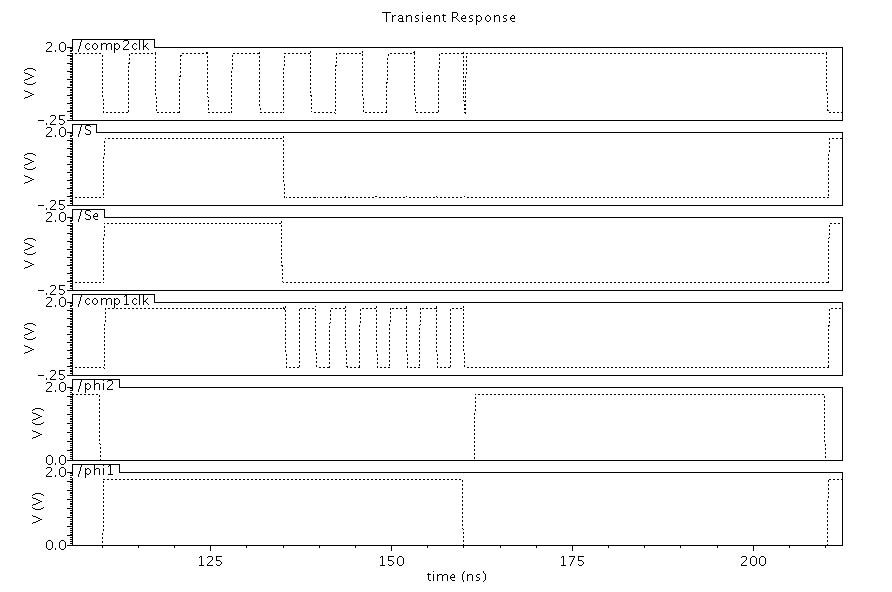
\includegraphics[width=\textwidth]{basicclocks}
\caption{Waveform of a Single Cycle of Design Clocks}
\label{fig:basicclocks}
\end{figure}
\section{Design of Single-Ended ADC}
With the calculation of all the general design parameters complete, the design could move into the circuit design and simulation phase. The first design was a single-ended one, as this design was easier to debug. Although all of the previous chapter's calculations assumed a differential design, only a few changes needed to be made to accommodate the single-ended design. First, the full-scale voltage would only be \SI{1}{\volt} for the single-ended design. Second, all noise calculations were done assuming differential capacitor arrays, so expected noise contributions had to be halved for the single-ended design. The operation of the first and second stage SAR ADCs follows the explanation in Section \ref{sec:saroperation}, with the operation expanded to six and seven bits, respectively. The first task in the single-ended design was to design the digital SAR control logic. Next, the clocking scheme, capacitor sizes, and digital logic were verified by using ideal component parameters. Once all of the surrounding logic had been verified, the calculated parameters from Section \ref{sec:designparameters} were put into the ideal models. With the calculated parameters, transient simulations were run to verify that the MDAC settling met the specifications from Section \ref{sec:idealotaparams}. Once adherence to the settling specification was verified, a longer simulation was run to obtain device SQDR. Once the 74 dB SQDR was achieved, noise simulations were run to ensure that the total input-referred noise met the design specifications. Once all this was complete, work moved on to the differential design.
\subsection{Single-Ended SAR Control Logic}
The SAR control logic determines the operation of all of the conversion switches in the design. In addition, it uses the comparator output to construct the digital output code of the ADC. All of the digital logic described in this section was designed at the gate level using standard cells. Due to the low speed, in digital terms, of the clocks in this design and the low complexity of the digital logic, minimum sized gates were used throughout the design. Using minimum sized gates decreases the dynamic power consumption of the digital blocks in the design.

The first-stage SAR logic was designed first with the intention of expanding the logic to the second stage. The SAR control logic governs the behavior of the $d_i$ switches in Figure \ref{fig:saradcex}. The first-stage control logic was implemented as a state machine with the negative edge of the SAR clock controlling state transitions. Table \ref{tab:stageonestatemachine} summarizes the operation of the SAR state machine. In this table, $C$ corresponds to the comparator output at the end of the previous state, and $d_ip$ corresponds to the $d_i$ signal maintaining its previous state. 
\begin{table}[htbp]
\renewcommand*\arraystretch{1.3}
\begin{center}
\begin{tabular}{|r|r|r|r|l|r|r|r|}
\hline
\multicolumn{ 2}{|c|}{State Outputs} & \multicolumn{ 6}{c|}{Switch Outputs} \\ \hline
\multicolumn{1}{|l|}{Current State} & \multicolumn{1}{l|}{Next State} & \multicolumn{1}{l|}{$d_{5}$} & \multicolumn{1}{l|}{$d_{4}$} & $d_{3}$ & \multicolumn{1}{l|}{$d_{2}$} & \multicolumn{1}{l|}{$d_{1}$} & \multicolumn{1}{l|}{$d_{0}$} \\ \hline
0 & 1 & 0 & 0 & \multicolumn{1}{r|}{0} & 0 & 0 & 0 \\ \hline
1 & 2 & 1 & 0 & \multicolumn{1}{r|}{0} & 0 & 0 & 0 \\ \hline
2 & 3 & $\overline{C}$ & 1 & \multicolumn{1}{r|}{0} & 0 & 0 & 0 \\ \hline
3 & 4 & $d_{5p}$ & $\overline{C}$ & \multicolumn{1}{r|}{0} & 0 & 0 & 0 \\ \hline
4 & 5 & $d_{5p}$ & $d_{4p}$ & \multicolumn{1}{r|}{$\overline{C}$} & 1 & 0 & 0 \\ \hline
5 & 6 & $d_{5p}$ & $d_{4p}$ & $d_{3p}$ & $\overline{C}$ & 1 & 0 \\ \hline
6 & 7 & $d_{5p}$ & $d_{4p}$ & $d_{3p}$ & \multicolumn{1}{l|}{$d_{2p}$} & $\overline{C}$ & 1 \\ \hline
7 & 0 & $d_{5p}$ & $d_{4p}$ & $d_{3p}$ & \multicolumn{1}{l|}{$d_{2p}$} & \multicolumn{1}{l|}{$d_{1p}$} & $\overline{C}$ \\ \hline
\end{tabular}
\end{center}
\caption{Stage One SAR Control Logic State Machine}
\label{tab:stageonestatemachine}
\end{table}
When the ADC is in the sampling phase, clock signal $S$ is active and all other switches are open. This is accomplished by gating all the $d_{i}$ and $\overline{d_{i}}$ switch control inputs with $\overline{S}$. During this phase, the SAR state machine is reset to its initial state.  Once the sampling phase ends, the first stage SAR clock, \emph{comp1clk}, falls, the state machine moves into State 1, and the SAR begins its conversion operation. For the state machine to complete all of its operations, seven \emph{comp1clk} falling edges are required. Once the state machine reaches State 7, it maintains its state until the next sampling clock rising edge. This state machine must hold its state throughout $\phi_{2}$ so that the residue voltage is properly amplified by the MDAC. Once the sampling clock rising edge occurs, the state machine is reset to State 0, and all of the SAR switches open. 

The SAR control logic for the second stage ADC is almost identical to the first stage. An additional state and digital output were added to accommodate the seven bit ADC. In this case, eight falling \emph{comp2clk} edges are required. Also, the second stage state machine is reset by the negative edge of $\phi_{2}$, which corresponds to the sampling phase of the second stage ADC. Other than these differences, the operation of the second stage SAR is identical to that of the first stage.
\subsection{Test Setups}
\label{sec:adcsimulations}
Before continuing with the discussion on simulating the ADC using ideal component parameters, it is worthwhile to discuss the simulation tests that were used throughout the design of this ADC. When evaluating the performance of the entire pipelined system, four main tests were used for all design iterations. The first was a short transient simulation to ensure that the MDAC output was settling properly and the digital outputs were being set properly. The next test was a longer transient simulation that was used to perform a DFT on the digital output. Once performance in these two simulations met specifications, two different types of noise simulations were run, in order to provide a means of verifying that the noise results were accurate. First, AC noise simulations were run on the ADC in both its sampling and amplification phases. Next, a transient periodic noise simulation was run on the ADC. Once transistor level models for the OTA had been integrated into the full ADC, power consumption simulations were also performed on the design. This section describes in more detail each of these simulations.
\subsubsection{Transient Settling Test}
\label{sec:transettling}
In this test, a full-scale voltage step was applied to the input of the ADC. The digital output was checked to ensure that the output was the maximum digital code from the ADC. If the digital output was not its maximum, this implied an error with the digital control logic that would be fixed. Next, the output of the MDAC at the end of $\phi_{2}$ was checked to ensure that the MDAC settling specifications were met. If the circuit was not settling properly, this meant that the \emph{Gain} or \emph{$g_{m}$} OTA model parameters were not large enough and needed to be corrected. In the case of differential designs, a full-scale negative input was also applied. If the digital output code was correct and the MDAC settled within specifications, this test was considered successful.
\subsubsection{Transient DFT Test}
\label{sec:transientdft}
 In this test an input sine wave with a frequency of (31/64)$\times$10 MHz was applied to the input of the ADC and the simulation is run for 64 cycles. Once the test is complete, a Matlab script is used to perform a 64-point DFT on the output samples and obtain an SQDR. This input frequency was chosen for a few reasons. First, this frequency is very close to the Nyquist frequency of the ADC, so the ADC is being tested close to its theoretical maximum frequency. Second, when capturing a 64-point DFT, exactly 31 cycles of this input frequency will be sampled. Having an integer number of periods ensures that no spectral leakage occurs in the DFT and therefore no windowing has to be applied to the input samples. Last, the number of cycles and the number of DFT samples is mutually prime in order to obtain random quantization noise. When the mutually prime criteria is not met, the quantization noise is more deterministic and periodic, so the DFT power is spread across fewer bins. If the SQDR meets specification, this test is considered passed. In terms of simulation using ideal components, an ideal SQDR for a 12 bit ADC of 74 dB was expected.
\subsubsection{AC Noise Analysis}
\label{sec:acnoisesim}
AC Noise analysis computes a static DC operating point, and computes an AC noise output power using this operating point. Since this ADC operates in two phases, the circuit schematics could not be used as designed when performing AC analysis. Two different schematics had to be created for simulation, one that models the device in its sampling phase, and one that models the device in its amplification phase. In the sampling phase a schematic similar to that in Figure \ref{fig:mdacsampling} was used. For the sampling phase AC noise analysis, the first stage capacitive network was fully modeled, not lumped together. Since the second stage capacitive array only contributes kT/C noise, it was modeled as a lumped capacitance. For the amplification phase AC noise analysis, a circuit similar to that of Figure \ref{fig:generalmdac}, with only the $\phi_{2}$ switches closed. The first stage capacitive array was again fully modeled, while the second-stage array was modeled with a lumped capacitance. The sum of the noise power from each of these simulations was the total ADC noise output power. If the output noise power was less than that defined in Table \ref{tab:maxoutputnoise}, this test was considered successful. A failure of this test meant that capacitor sizes likely needed to be enlarged, or OTA noise needed to be decreased by increasing OTA $g_{m}$. Another signal that something was wrong with the simulation was if it did not match the next test, the AC periodic noise simulation. In the case that the simulations did not match, an issue with the simulation setup was generally assumed.
\subsubsection{AC Periodic Noise Analysis}
In this test, a periodic steady state (PSS) simulation is combined with a transient periodic noise (PNOISE) simulation to give a calculation of the total noise power. In this case, the circuit simulator tries to solve for the periodic operation of the circuit. Once a periodic steady state solution is achieved, it calculates the noise across the period at a given time point. The point chosen for this simulation was at the end of the amplification phase. This simulation was the most prone to having setup issues due to the large number of required run settings. An excellent overview of using PSS and PNOISE analysis is in~\cite{simswitchcap} and the recommendations from this paper were used in setting up the simulation correctly. Using AC noise simulations, the number of sidebands and maximum AC frequency to use were determined for this design. Table \ref{tab:pnoiseparams} summarizes the PNOISE parameters used for all simulations of this design.
\begin{table}[htbp]
\begin{center}
\begin{tabular}{|l|l|}
\hline
Parameter & Value \\ \hline
Beat Frequency & \SI{5}{\mega\hertz} \\ \hline
Accuracy & conservative \\ \hline
Maximum Sidebands & 400 \\ \hline
\end{tabular}
\caption{PNOISE Simulation Setup}
\label{tab:pnoiseparams}
\end{center}
\end{table}
\subsubsection{Power Consumption Test}
\label{sec:powerconsumptiontest}
Although the power consumption test did not become truly relevant until the OTA had been integrated into the design, it is worthwhile to discuss it in the context of the full ADC design. For this test, the ADC was stimulated with the same input from the transient DFT test described in Section \ref{sec:transientdft}. While the power consumption of the ADC is generally dominated by the static bias current of the OTA, the switching activity on the digital control logic and the sampling capacitors contributes some dynamic power. The amount of switching activity is dependent on the input signal presented to the ADC. In order to obtain an accurate estimation of total current consumption a number of input amplitudes needs to be applied to the ADC. In order to achieve this, a transient test is run with a duration of ten sampling cycles. This corresponds to just under five cycles of the input sinusoid, so a good distribution of input values should be obtained. The average current through the supply voltage is calculated and multiplied by the supply current value in order to obtain the total power consumption.
\subsection{Simulation Using Ideal OTA Model Parameters}
After designing the full single-ended ADC circuit, performance testing could commence. In an effort to separate the verification of the SAR operation from the verification of the pipeline block parameters, ideal OTA model parameters were used in the first design simulations. In this case, ideal OTA parameters refers to using a very large gain and transconductance, so that the error in the MDAC output is negligible. By doing this, any errors in the digital output could only be the result of bugs in SAR sub-ADCs. During this simulation phase, the transient settling and transient DFT tests were used to verify proper operation.

A number of bugs were discovered during this testing phase. A large number of these had to do with errors in the state machine logic that were easily caught during the initial transient settling test. Two bugs relating to the relationship between the clock domains proved to be the most difficult to debug. 

First, the time between the last decision of the first-stage SAR ADC and the rising edge of the $\phi_{2}$ clock was not great enough. This meant that the last DAC output voltage from the SAR was not fully settled by the time amplification started, causing errors in the residue voltage that was initially amplified. Two solutions were considered to fix this. First, the \emph{comp1clk} speed could be increased to \SI{280}{\mega\hertz} to allow for an extra clock cycle between the last decision phase and the start of the amplification phase. This option would required a slight redesign of the first stage state machine, as well as an increase in comparator decision time of over 15\%. Second, the start of the amplification phase could be delayed slightly to allow adequate time for the last DAC voltage to settle before amplification started. This solution would mean decreasing the overall amplification time slightly, which would require an increase in the OTA transconductance to maintain the same dynamic error. Simulations showed that increasing the time between the last SAR decision and the amplification phase to \SI{1.3}{\nano\second} allowed the DAC output voltage to fully settle and for the amplified voltage to be within specification for all samples. This caused a decrease in the amplification time from \SI{48.8}{\nano\second} to \SI{48.5}{\nano\second}. Recalculating the required OTA bandwidth and transconductance using Equations \ref{eq:idealgm} and \ref{eq:fcdynamicerror} showed that the transconductance only needed to increase to \SI{3.3}{\milli\siemens} to maintain the same dynamic error. Since the required increase in OTA transconductance was minimal, decreasing the amplification time slightly was the chosen solution to this issue. 

Next, an issue with the second-stage SAR clocking was found. The time between the last falling edge of the second stage SAR clock and the $\phi_{2}$ signal was causing the state machine to reset before the final bit decision was captured. This caused the least significant bit of the digital output to always be 0. Since the second stage comparator already had a lower speed requirement than that of the first-stage, it was decided to add another clock cycle to the second stage SAR ADC. This caused an increase in \emph{comp2clk} from \SI{140}{\mega\hertz} to \SI{160}{\mega\hertz}. Some changes to the control logic were likely required to implement the differential SAR, so it was decided to fix this issue without raising the clock frequency at that time. Figure \ref{fig:fixedclocks} shows the modifications made to the clocking scheme. Markers \emph{M0} and \emph{M1} in Figure \ref{fig:fixedclocks} show the time difference between the falling edge of \emph{comp1clk} and the rising edge of $\phi_{2}$. Markers \emph{M1} and \emph{M2} show the reduction in amplification time. The waveform for \emph{comp2clk} shows the additional clock cycle that was added. 
\begin{figure}[htbp]
\centering
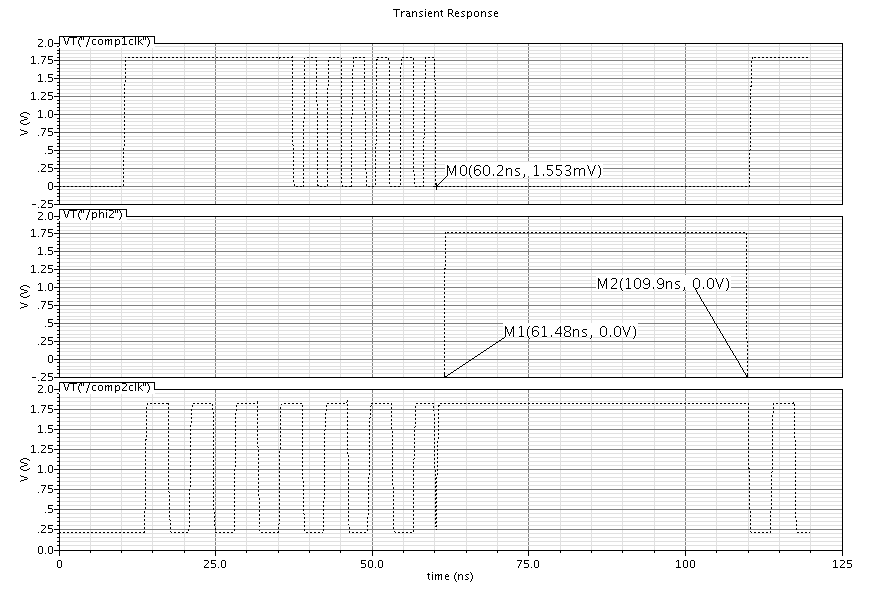
\includegraphics[width=\textwidth]{clockfixes}
\caption{Clocking Modifications Made for Ideal Component Parameter Design}
\label{fig:fixedclocks}
\end{figure}

Once these bugs were fixed, the transient DFT simulation was run on the design. Figure \ref{fig:idealparamsingledft} shows the final DFT output from this iteration of the design. With an SQDR of \SI{74}{\decibel}, this iteration of the design could be considered complete.
\begin{figure}[htbp]
\centering
\includegraphics[width=\textwidth]{ideal_single_two_stage_douttotal_fft}
\caption{Final DFT Output of Single-Ended Model With Ideal OTA Parameters} 
\label{fig:idealparamsingledft}
\end{figure}
\subsection{Simulation with Calculated OTA Model Parameters}
Once the ideal SQDR was achieved with ideal OTA model parameters, the calculated model parameters were used and simulations were run again. In this case, the transient settling simulation and transient DFT simulations were run first. After these simulations, the noise simulations were run to verify the noise behavior of the circuit.

The first verification step was running transient simulations. Figure \ref{fig:singleendedtran} shows the output voltage of the MDAC during the amplification stage with full-scale voltage input. At the end of the amplification phase, the MDAC output voltage is \SI{848.5}{\milli\volt}
\begin{figure}[htbp]
\centering
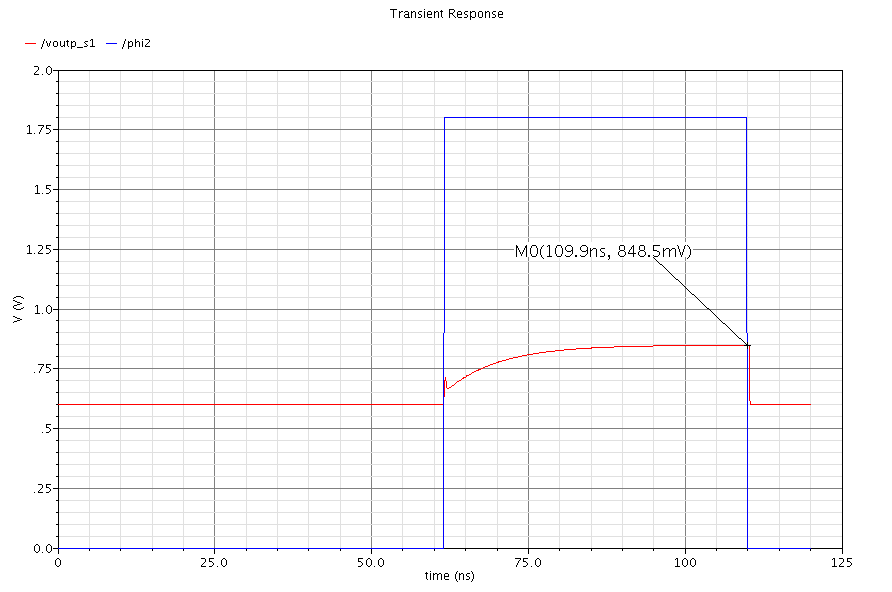
\includegraphics[width=\textwidth]{transingle}
\caption{Transient Settling of Single-Ended ADC With Ideal Components} 
\label{fig:singleendedtran}
\end{figure}
 With a full-scale input, the expected MDAC output is:
\begin{equation}
\label{eq:fullscalemdacoutput}
V_{MDAC} = \dfrac{V_{ref}}{4} + V_{cm}
\end{equation}
where $V_{cm}$ is the common-mode voltage. In this case, the common-mode voltage is set to \SI{600}{\milli\volt}, the expected output voltage is \SI{850}{\milli\volt}. From Figure \ref{fig:singleendedtran}, the settling error is \SI{-1.5}{\milli\volt}. The maximum error is the sum of the static and dynamic error specifications, or \SI{2.4}{\milli\volt}. The full-scale input error was within this error envelope, so the testing moved on to transient DFT.

The initial transient DFT simulation yielded an SQDR of 74 dB, which met the required specification. After achieving this metric, the switch resistances were increased in order to reduce the size and power consumption of the switches when implemented as transistors. After running a number of times, a sampling switch resistance of \SI{400}{\ohm} was found to still produce SQDR. All other switch resistances were set to \SI{500}{\ohm}. Figure \ref{fig:idealsingletwostagecalcparams} shows the final DFT from these simulation runs.
\begin{figure}[htbp]
\centering
\includegraphics[width=\textwidth]{idealsinglecalparamsdft}
\caption{DFT of Single-Ended ADC With Calculated Parameters} 
\label{fig:idealsingletwostagecalcparams}
\end{figure}

After obtaining an SQDR of 74 dB from the transient DFT simulation, noise simulations could be run. First the AC sampling and amplification phase noise simulations were run. Figures \ref{fig:acsamplenoisesingle} and \ref{fig:acholdnoisesingle} are graphs of the integrated output noise obtained from these simulations.
\begin{figure}[htbp]
\centering
\includegraphics[width=\textwidth]{acsamplenoisesingle}
\caption{AC Noise During Sampling Phase of Single-Ended ADC} 
\label{fig:acsamplenoisesingle}
\end{figure}
\begin{figure}[htbp]
\centering
\includegraphics[width=\textwidth]{acholdnoisesingle}
\caption{AC Noise During Amplification Phase of Single-Ended ADC} 
\label{fig:acholdnoisesingle}
\end{figure}
Additionally, an AC noise simulation was run with the OTA noise generator turned off, in order to compare the calculated OTA noise power to that of the simulation. These results are summarized in Table \ref{tab:acnoisesummarysingle}.
\begin{table}[htbp]
\renewcommand*\arraystretch{1.3}
\begin{center}
\begin{tabularx}{\linewidth}{|l|X|X|X|X|}
\hline
Setup & AC Sampling Noise (\si{\milli\volt_{rms}}) & Total AC Hold Noise  (\si{\milli\volt_{rms}}) & AC Hold OTA Noise  (\si{\milli\volt_{rms}}) & AC Total Noise  (\si{\milli\volt_{rms}}) \\ \hline
Simulation & 1.07 & 0.44 & 0.32 & 1.16 \\ \hline
Calculation & 1.07 & 0.41 & 0.33 & 1.10 \\ \hline
Design Target & 1.07 & 1.56 & 1.51 & 1.89 \\ \hline
Error (\%) & 0.31 & 7.10 & -1.69 & 5.63 \\ \hline
Headroom (\%) & -0.48 & 72.20 & 78.66 & 38.89 \\ \hline
\end{tabularx}
\end{center}
\caption{Single-Ended AC Output Noise Power Summary}
\label{tab:acnoisesummarysingle}
\end{table}
The only noise value that significantly diverges from its calculated value is that of the AC hold phase noise, despite the OTA noise being very close to its calculated value. It was first thought that the $C_{s2}$ noise contribution may not have been calculated correctly. To test this, all noise sources were turned off except for the switch at the output of the stage two capacitive array. The output noise in this case matched the calculated kT/C noise, so this was determined to not be the cause of error. Further simulations revealed that the switch resistances at the input of the MDAC were contributing significant noise, which was not accounted for in the noise calculations. Since both the hold noise power and the total noise power were well within their budgets, the switch resistance was not changed as a result of this finding. While no changes were made, the switch resistance was kept as a knob to tune the total output noise power if, after implementing the transistor level design, total output noise became an issue. Next, a PSS/PNOISE simulation was run to verify the AC noise simulations. Figure \ref{fig:pnoisesingle} shows the integrated root-mean-square (RMS) output noise voltage from this simulation. 
\begin{figure}[htbp]
\centering
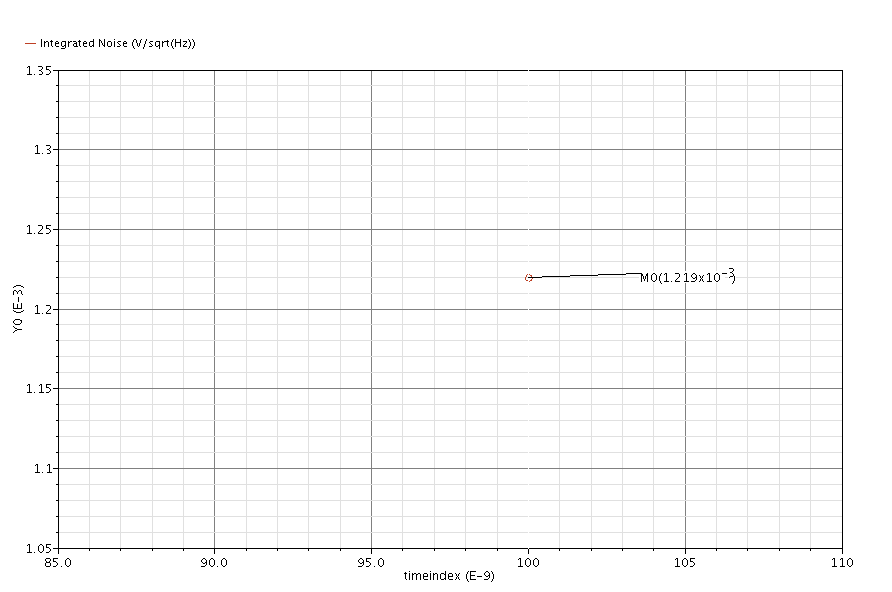
\includegraphics[width=\textwidth]{pnoisesingle}
\caption{Single-Ended PNOISE Simulation Result} 
\label{fig:pnoisesingle}
\end{figure}
Table \ref{tab:pnoisesummarysingle} translates this result into an output noise power and compares it to that from the AC simulations.
\begin{table}[htbp]
\begin{center}
\begin{tabularx}{\linewidth}{|l|X|X|X|}
\hline
Setup & Total Noise Power (\si{\milli\volt_{rms}}) & Error vs Calculation (\%) & Error vs AC Simulation (\%) \\ \hline
PNOISE Simulations & 1.22 & 6.69 & 5.44 \\ \hline
\end{tabularx}
\end{center}
\caption{Single-Ended PNOISE Output Noise Summary}
\label{tab:pnoisesummarysingle}
\end{table}
The PNOISE simulations show good agreement with both the AC Simulations and the calculations. With good agreement between both simulations and the calculations, as well as a total output noise power that was well within budget, the noise simulations were considered a success.

With both noise simulations and transient performance simulations complete, a full SNDR of the single-ended system could be calculated. Solving for the distortion and quantization noise power in Equation \ref{eq:sqdr} yields: 
\begin{align}
\label{eq:pqplusdissingle}
P_{qnoise}+P_{distortion} &= \dfrac{\dfrac{1}{2}\left(\dfrac{V_{FS}}{2}\right)^{2}}{SQDR} \\
\nonu &= \SI{4.94}{\square\nano\volt}
\end{align}
Since the PNOISE result gave the highest output noise, that was the value used for the SNDR calculation. Referring the noise power to the input produced a noise power of \SI{5.82}{\square\nano\volt}. Using Equation \ref{eq:sndr}, the calculated SNDR was:
\begin{equation}
\label{eq:sndrsingle}
SNDR_{SE} = \SI{70.7}{\decibel}
\end{equation}
From Equation \ref{eq:enob}, this translates to an ENOB of 11.4 bits. 
\section{Design of Fully Differential ADC With Ideal Components}
Once the single-ended design was complete, it needed to be expanded to a differential design. Expanding to a differential design involved mirroring the sub-ADC capacitor arrays to enable a positive and negative input, as well as using the differential OTA model for the MDAC. In addition, to accommodate the differential design, the SAR control logic had to be slightly redesigned. The parameters for all of the design blocks and all of the capacitor sizes were able to remain the same, however. The differential design followed a similar design cycle as that of the single-ended design. 
\subsection{Expanding the SAR ADCs to Accept Differential Inputs}
In order for the SAR ADC to accept a differential signal, the voltage reference had to be split into a positive reference voltage and a negative reference voltage. The relationship between these voltages is:
\begin{equation}
\label{eq:vrefp}
V_{refp} = V_{cm}+\dfrac{V_{ref}}{2}
\end{equation}
\begin{equation}
\label{eq:vrefn}
V_{refn} = V_{cm}-\dfrac{V_{ref}}{2}
\end{equation}
Figure \ref{fig:diffsaradc} is an expansion of \ref{fig:saradcdummylsb} to include differential inputs. While Figure \ref{fig:diffsaradc} still uses the dummy LSB capacitor to achieve an extra bit of resolution, the resolution of the ADC has been lowered to two bits. 
\begin{figure}[htbp]
\centering
\newcommand{\colspacing}{4.5}
\newcommand{\colfourspacing}{2}
\newcommand{\rowspacing}{-1}
\newcommand{\negrowspacing}{1}
\newcommand{\digitalrel}{-0.5}
\newcommand{\switchrelctl}{-0.1}
\newcommand{\switchrelspace}{-1}
\newcommand{\labelrelspace}{-1}
\newcommand{\rowone}{0}
\newcommand{\rowtwo}{\rowone+\rowspacing}
\newcommand{\rowthree}{\rowtwo+\rowspacing}
\newcommand{\rowthreehalf}{\rowthree+\rowspacing}
\newcommand{\rowfour}{\rowthreehalf+\rowspacing}
\newcommand{\rowfive}{\rowfour+\rowspacing}
\newcommand{\rowsix}{\rowfive+\rowspacing}
\newcommand{\rowseven}{\rowsix+\rowspacing}
\newcommand{\roweight}{\rowseven+\rowspacing}
\newcommand{\rownine}{\roweight+\rowspacing}
\newcommand{\rowten}{\rownine+\rowspacing}
\newcommand{\roweleven}{\rowten+\rowspacing}
\newcommand{\rowtwelve}{\roweleven+\rowspacing}
\newcommand{\colone}{-2}
\newcommand{\coltwo}{\colone+\colspacing}
\newcommand{\colthree}{\coltwo+\colspacing}
\newcommand{\colfour}{\colthree+\colfourspacing}
\newcommand{\colfive}{\colfour+\colfourspacing}
\newcommand{\colsix}{\colfive+\colfourspacing}
\begin{circuitikz} 
\draw
%in connection
	(\colone, \rowone) node[anchor=south] {$V_{inp}$} -- (\colthree, \rowone)
%vcm connection
	(\colone, \rowtwo) node[anchor=south]  {$V_{cm}$} -- (\colfour+\switchrelspace, \rowtwo)
%vrefp connection
	(\colone, \rowthree) node[anchor=south]  {$V_{refp}$} -- (\coltwo+2*\switchrelspace, \rowthree)
%vrefn connection
	(\colone, \rowthreehalf) node[anchor=south] {$V_{refn}$} -- (\coltwo+3*\switchrelspace, \rowthreehalf)
%bit1 switch connections
	%sample switch
	(\coltwo, \rowfour)  to[cspst, l=$S$] (\coltwo, \rowfive)
	(\coltwo, \rowfour) to [short, -*] (\coltwo, \rowone)
	%vcm switch
	(\coltwo, \rowfour) ++(\switchrelspace, 0) to [cspst, l=$G$]  ++(0, \rowspacing) to [short, -*] ++(0,0)
	(\coltwo, \rowfour) ++(\switchrelspace, 0) to [short, -*] ++(0, -3*\rowspacing)
	%vrefp switch
	(\coltwo, \rowfour) ++(2*\switchrelspace, 0) to [cspst, l=$d_{1}$]  ++(0, \rowspacing) to [short, *-] ++(0, 0) 
	(\coltwo, \rowfour) ++(2*\switchrelspace, 0) to [short] ++(0, -2*\rowspacing)
	(\coltwo, \rowfive) -- ++(2*\switchrelspace, 0)
	%vrefn switch
	(\coltwo, \rowfour) ++(3*\switchrelspace, 0) to [cspst, l=$\overline{d_{1}}$]  ++(0, \rowspacing)
	(\coltwo, \rowfour) ++(3*\switchrelspace, 0) to [short] ++(0, -1*\rowspacing)
	(\coltwo, \rowfive) -- ++(3*\switchrelspace, 0)
%bit1 cap
	(\coltwo, \rowfive) ++(\switchrelspace, 0) to [C, l=C] ++(0, \rowspacing)
%dummy LSB switch connections
	%sample switch
	(\colthree, \rowfour)  to[cspst, l=$S$] (\colthree, \rowfive)
	(\colthree, \rowfour) to [short] (\colthree, \rowone)
	%vcm switch
	(\colthree, \rowfour) ++(\switchrelspace, 0) to [cspst, l=$G$]  ++(0, \rowspacing) to [short, -*] ++(0,0) 
	(\colthree, \rowfour) ++(\switchrelspace, 0) to [short, -*] ++(0, -3*\rowspacing)
	%vrefp switch
	(\colthree, \rowfour) ++(2*\switchrelspace, 0) to [cspst, l=$d_{0}$]  ++(0, \rowspacing) to [short, *-] ++(0, 0) 
	(\colthree, \rowfour) ++(2*\switchrelspace, 0) to [short] ++(0, -2*\rowspacing)
	node[anchor=south] {$V_{refp}/2$}
	(\colthree, \rowfive) -- ++(2*\switchrelspace, 0)
	%vrefn switch
	(\colthree, \rowfour) ++(3*\switchrelspace, 0) to [cspst, l=$\overline{d_{0}}$]  ++(0, \rowspacing)
	(\colthree, \rowfour) ++(3*\switchrelspace, 0) to [short] ++(0, -1*\rowspacing)
	node[anchor=south] {$V_{refn}/2$}
	(\colthree, \rowfive) -- ++(3*\switchrelspace, 0)
%dummy lsb cap
	(\colthree, \rowfive) ++(\switchrelspace, 0) to [C, l=C] ++(0, \rowspacing)  to [short, *-] ++(0, 0)
	(\colthree, \rowfive) -- ++(\switchrelspace, 0)
%comp input vcm switch
	(\colfour, \rowfour) ++(\switchrelspace, 0) to [cspst, l=$S$]  ++(0, \rowspacing)
	(\colfour, \rowfour) ++(\switchrelspace, 0) to [short] ++(0, -3*\rowspacing)
	(\colfour, \rowfive) ++(\switchrelspace, 0) -- ++(0, \rowspacing)  to [short, -*] ++(0,0)
	(\coltwo+\switchrelspace, \rowsix) -- (\colfour, \rowsix)
	node[plain amp, anchor=-] (comp) {}
	(comp.-) ++(-0.5, 0) node[anchor=south west] {X}
	(comp.center) ++(-0.1,0) node[anchor=center] {Comp}
	(comp.out) node[anchor=south] {$d_{n}$}
%neg comp input vcm switch
	(comp.+) ++(-0.5, 0) node[anchor=south west] {Y} -- (\colfour, \rowseven) --
	++(\switchrelspace, 0) to [short, *-] ++(0,-1*\negrowspacing) to [cspst, l=$S$] ++(0, -1*\negrowspacing)
	(\colfour, \roweight) ++(\switchrelspace, 0) to [short] ++(0, -3*\negrowspacing)
	(\colfour, \rowfive) ++(\switchrelspace, 0) -- ++(0, \negrowspacing)
	(\coltwo+\switchrelspace, \rowseven) -- (\colfour, \rowseven)
%in connection
	(\colone, \rowtwelve) node[anchor=south] {$V_{inn}$} -- (\colthree, \rowtwelve)
%vcm connection
	(\colone, \roweleven) node[anchor=south]  {$V_{cm}$} -- (\colfour+\switchrelspace, \roweleven)
%vrefn connection
	(\colone, \rowten) node[anchor=south]  {$V_{refn}$} -- (\coltwo+2*\switchrelspace, \rowten)
%vrefp connection
	(\colone, \rownine) node[anchor=south] {$V_{refp}$} -- (\coltwo+3*\switchrelspace, \rownine)
%dummy LSB switch connections
	%sample switch
	(\colthree, \roweight)  to[cspst, l=$S$] (\colthree, \rownine)
	(\colthree, \roweight) to [short] (\colthree, \rowtwelve)
	%vcm switch
	(\colthree, \roweight) ++(\switchrelspace, 0) to [short, -*] ++(0,0) to [cspst, l=$G_{1}$]  ++(0, -\negrowspacing)
	(\colthree, \roweight) ++(\switchrelspace, 0) to [short, -*] ++(0, -3*\negrowspacing)
	%vrefn switch
	(\colthree, \roweight) ++(2*\switchrelspace, 0) to [short, *-] ++(0, 0) to [cspst, l=$d_{0}$]  ++(0, -1*\negrowspacing)
	(\colthree, \roweight) ++(2*\switchrelspace, 0) to [short] ++(0, -2*\negrowspacing)
	node[anchor=north] {$V_{refn}/2$}
	(\colthree, \roweight) -- ++(2*\switchrelspace, 0)
	%vrefp switch
	(\colthree, \roweight) ++(3*\switchrelspace, 0) to [cspst, l=$\overline{d_{0}}$]  ++(0, -1*\negrowspacing)
	(\colthree, \roweight) ++(3*\switchrelspace, 0) to [short] ++(0, -1*\negrowspacing)
	node[anchor=north] {$V_{refp}/2$}
	(\colthree, \roweight) -- ++(3*\switchrelspace, 0)
%dummy lsb cap
	(\colthree, \rowseven) ++(\switchrelspace, 0) to [C, l=C] ++(0, -\negrowspacing)
	(\colthree, \rowseven) -- ++(\switchrelspace, 0)
%bit1 switch connections
	%sample switch
	(\coltwo, \roweight)  to[cspst, l=$S$] (\coltwo, \rownine)
	(\coltwo, \roweight) to [short, -*] (\coltwo, \rowtwelve)
	%vcm switch
	(\coltwo, \roweight) ++(\switchrelspace, 0) to [short, -*] ++(0,0) to [cspst, l=$G_{0}$]  ++(0, -\negrowspacing)
	(\coltwo, \roweight) ++(\switchrelspace, 0) to [short, -*] ++(0, -3*\negrowspacing)
	%vrefn switch
	(\coltwo, \roweight) ++(2*\switchrelspace, 0) to [short, *-] ++(0, 0) to [cspst, l=$d_{1}$]  ++(0, -\negrowspacing)
	(\coltwo, \roweight) ++(2*\switchrelspace, 0) to [short] ++(0, -2*\negrowspacing)
	(\coltwo, \roweight) -- ++(2*\switchrelspace, 0)
	%vrefp switch
	(\coltwo, \roweight) ++(3*\switchrelspace, 0) to [cspst, l=$\overline{d_{1}}$]  ++(0, -\negrowspacing)
	(\coltwo, \roweight) ++(3*\switchrelspace, 0) to [short] ++(0, -1*\negrowspacing)
	(\coltwo, \roweight) -- ++(3*\switchrelspace, 0)
%bit1 cap
	(\coltwo, \roweight) ++(\switchrelspace, 0) to [C, l=C] ++(0, \negrowspacing)
;
\end{circuitikz}
\caption{Example Two Bit Differential SAR ADC}
\label{fig:diffsaradc}
\end{figure}
The switches connecting the bottom plate of the sampling capacitors is now controlled by a new signal, $G$. At the end of the sampling phase, the $G$ signal is asserted for all bits, and all other switches are open. Using an analysis similar to the analysis from Section \ref{sec:saroperation}, the expression for the comparator output at the end of the first conversion step is:
\begin{equation}
\label{sard1diff}
d_{n} =	\begin{cases}
				0 & \mbox{if } V_{inp} > V_{inn} \\[0.5em]
				1 & \mbox{if } V_{inp} < V_{inn}
			\end{cases}
\end{equation}
Once again, the digital output of the ADC is the logical not of the comparator output. After the first conversion step, $G_{1}$ is deasserted, and the expression for the differential voltage at the comparator inputs is:
\begin{equation}
\label{eq:vdiffsarout}
V_{diff,cin} = \begin{cases}
				(V_{inp}-V_{inn}) - \dfrac{V_{ref}}{2} & \mbox{if } d_{1} = 1 \\[0.5em]
				(V_{inp}-V_{inn}) + \dfrac{V_{ref}}{2} & \mbox{if } d_{1} = 0
			\end{cases}
\end{equation}
The expression for the $d_{0}$ at the end of the second conversion stage is:
\begin{equation}
d_{0} =	\begin{cases}
				1 & \mbox{if } V_{inp}-V_{inn} > \dfrac{\pm V_{ref}}{2} \\[0.5em]
				0 & \mbox{if } V_{inp}-V_{inn} < \dfrac{\pm V_{ref}}{2}
			\end{cases}
\end{equation}
where $V_{ref}$ is positive if $d_{1}$ is 1 and negative if $d_{1}$ is 0. Conversion could continue in this manner for an arbitrary number of stages. 
\subsection{Design of Differential Control Logic}
The expansion to differential outputs necessitated two major changes in the SAR control logic. First, a new control signal has been added to control the switches connected to the common-mode input. These switches must stay asserted until after the corresponding bit decision stage. Additionally, the first decision stage of the differential ADC requires that only $G_{i}$ signals be asserted, which is different than that of the single-ended stage.  In addition to these required changes, some design issues that were encountered during the single-ended design phase needed to be addressed. The reason the additional clock cycle needed to be added to the second-stage ADC is that the state machine was being asynchronously reset by the rising edge of the sampling clock signal. This asynchronous behavior was removed during the design of the differential control logic. The state machine would now reset itself synchronously, so issues between the clock domains were removed and the second stage sampling clock frequency could be restored to \SI{140}{\mega\hertz}. Also, flip-flops separate from the normal control logic were used to store the digital output codes, allowing for easier sampling of the digital data. 

Table \ref{tab:statemachinedoutdiff} shows the digital outputs, $d_{i}$, in terms of the differential SAR state machine. Table \ref{tab:statemachinegdiff} shows the common-mode switch control output, $G$, in terms of the differential SAR state machine. The $G_{i}$, $d_{i}$, and $\overline{d_{i}}$, control signals must all be gated by the sampling clock of the sub-ADC, so that only the input sampling switch is closed during the sampling phase. The first and second stage control logic had only two differences. First the the second stage has an extra state to account for the extra conversion step required. Second, the sampling clock and the SAR conversion clocks for the two stages are different, although the internal behavior in response to these clocks is exactly the same. At the first falling edge of the SAR conversion clock, the state machine moves from state 6, or 7, to state 0 and conversion begins. Conversion ends when the state machine reaches state 6, or 7.
\begin{table}[htbp]
\renewcommand*\arraystretch{1.3}
\begin{center}
\begin{tabular}{|r|r|r|r|l|r|r|r|}
\hline
\multicolumn{1}{|l|}{Current State} & \multicolumn{1}{l|}{Next State} & \multicolumn{1}{l|}{$d_{5}$} & \multicolumn{1}{l|}{$d_{4}$} & $d_{3}$ & \multicolumn{1}{l|}{$d_{2}$} & \multicolumn{1}{l|}{$d_{1}$} & \multicolumn{1}{l|}{$d_{0}$} \\ \hline
0 & 1 & 0 & 0 & \multicolumn{1}{r|}{0} & 0 & 0 & 0 \\ \hline
1 & 2 & $\overline{C}$ & 0 & \multicolumn{1}{r|}{0} & 0 & 0 & 0 \\ \hline
2 & 3 & $d_{5p}$ & $\overline{C}$ & \multicolumn{1}{r|}{0} & 0 & 0 & 0 \\ \hline
3 & 4 & $d_{5p}$ & $d_{4p}$ & \multicolumn{1}{r|}{$\overline{C}$} & 0 & 0 & 0 \\ \hline
4 & 5 & $d_{5p}$ & $d_{4p}$ & $d_{3p}$ & $\overline{C}$ & 0 & 0 \\ \hline
5 & 6 & $d_{5p}$ & $d_{4p}$ & $d_{3p}$ & \multicolumn{1}{l|}{$d_{2p}$} & $\overline{C}$ & 0 \\ \hline
6 & 7 & $d_{5p}$ & $d_{4p}$ & $d_{3p}$ & \multicolumn{1}{l|}{$d_{2p}$} & \multicolumn{1}{l|}{$d_{1p}$} & $\overline{C}$ \\ \hline
\end{tabular}
\end{center}
\caption{Differential ADC Digital Output State Machine}
\label{tab:statemachinedoutdiff}
\end{table}

\begin{table}[htbp]
\begin{center}
\begin{tabular}{|r|r|r|r|r|r|r|r|}
\hline
\multicolumn{1}{|l|}{Current State} & \multicolumn{1}{l|}{Next State} & \multicolumn{1}{l|}{$G_{5}$} & \multicolumn{1}{l|}{$G_{4}$} & \multicolumn{1}{l|}{$G_{3}$} & \multicolumn{1}{l|}{$G_{2}$} & \multicolumn{1}{l|}{$G_{1}$} & \multicolumn{1}{l|}{$G_{0}$} \\ \hline
0 & 1 & 1 & 1 & 1 & 1 & 1 & 1 \\ \hline
1 & 2 & 0 & 1 & 1 & 1 & 1 & 1 \\ \hline
2 & 3 & 0 & 0 & 1 & 1 & 1 & 1 \\ \hline
3 & 4 & 0 & 0 & 0 & 1 & 1 & 1 \\ \hline
4 & 5 & 0 & 0 & 0 & 0 & 1 & 1 \\ \hline
5 & 6 & 0 & 0 & 0 & 0 & 0 & 1 \\ \hline
6 & 7 & 0 & 0 & 0 & 0 & 0 & 0 \\ \hline
\end{tabular}
\end{center}
\caption{Common-Mode Switch Control Output State Machine}
\label{tab:statemachinegdiff}
\end{table}
\subsection{Simulation Using Ideal OTA Model Parameters}
Similar to the design of the single-ended ADC, ideal OTA model parameters were used in order to verify the SAR operation. This phase was much shorter than in the single-ended case, as almost all of the bugs that were found were in the control logic and fixing them was straightforward. The amplification phase had to be shortened by another \SI{100}{\pico\second} in order for the last bit decision to fully settle. This slight decrease in the amplification phase did not necessitate any change in the OTA transconductance. By the end of this phase, the SQDR was once again 74 dB.
\subsection{Simulation with Calculated OTA Model Parameters}
After obtaining an ideal SQDR with the ideal OTA model parameters, the design was put through the same battery of tests that the single-ended design was put through. Transient simulations ensured that distortion power did not negatively effect the ADC performance, and then noise simulations were performed to ensure that the output noise was within its budget.

The transient settling simulation was the same as in the single-ended case, except that an input with the maximum negative magnitude and the maximum positive magnitude was used to ensure that the settling was not affected by signal polarity. Figures \ref{fig:tranposdiff} and \ref{fig:trannegdiff} are the graphs of the transient settling with a full-scale positive input and full-scale negative input, respectively.
\begin{figure}[htbp]
\centering
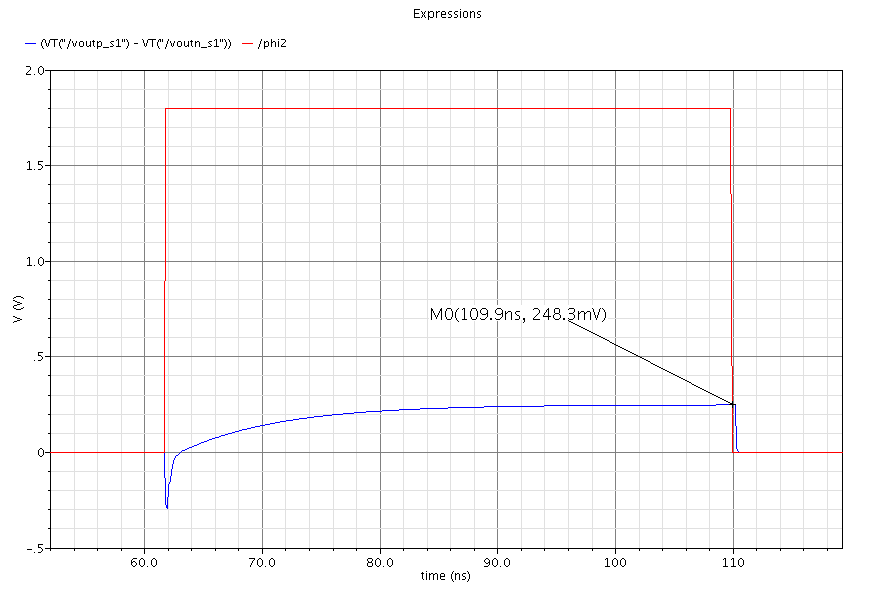
\includegraphics[width=\textwidth]{tranposdiff}
\caption{Transient Settling of Differential ADC With Ideal Components With Full-Scale Positive Input Voltage} 
\label{fig:tranposdiff}
\end{figure}
\begin{figure}[htbp]
\centering
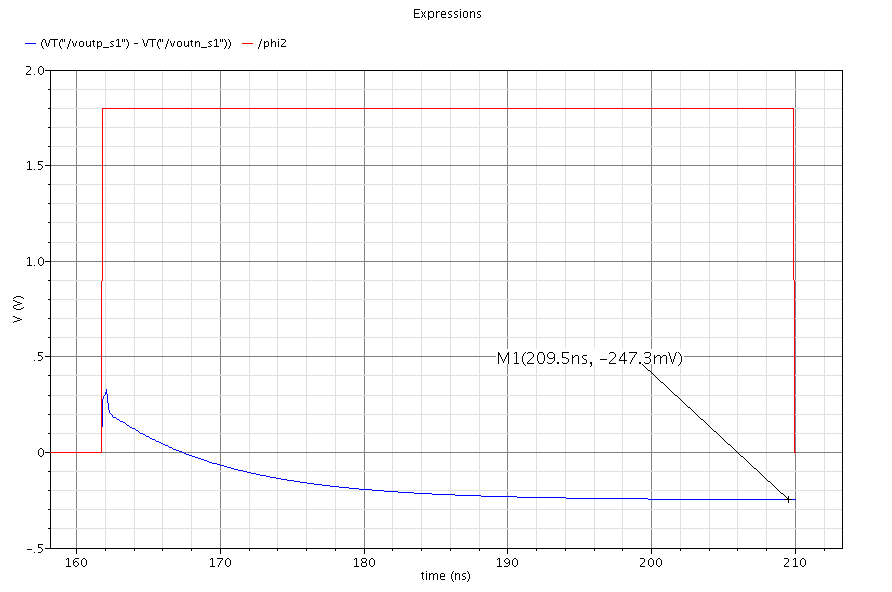
\includegraphics[width=\textwidth]{trannegdiff}
\caption{Transient Settling of Differential ADC With Ideal Components With Full-Scale Negative Input Voltage} 
\label{fig:trannegdiff}
\end{figure}
In the case of the positive input, the settling error is \SI{-1.7}{\milli\volt}. In the case of the negative input, the transient settling error is \SI{2.7}{\milli\volt}. In both of these cases, the settling error is within the maximum settling error envelope.

After verifying that the MDAC was settling properly, the DFT simulations were run. These simulations yielded an SQDR of 74 dB on the first run. Some additional runs were performed, however, to try to adjust the size of the sampling switches. In the case of the differential design, all switches were able to be sized with an on resistance of \SI{500}{\ohm}. Figure \ref{fig:fftfinaldiff} shows the DFT results from the final run of the differential simulation.
\begin{figure}[htbp]
\centering
\includegraphics[width=\textwidth]{ideal_diff_two_stage_douttotal_fft}
\caption{DFT of Differential ADC With Calculated Model Parameters} 
\label{fig:fftfinaldiff}
\end{figure}

With the transient performance meeting specification, the final step in the verification of the differential design was the noise simulations. Graphs of the simulation results from the AC noise simulations are given in Figures \ref{fig:acsamplenoisediff} and \ref{fig:acholdnoisediff}. 
\begin{figure}[htbp]
\centering
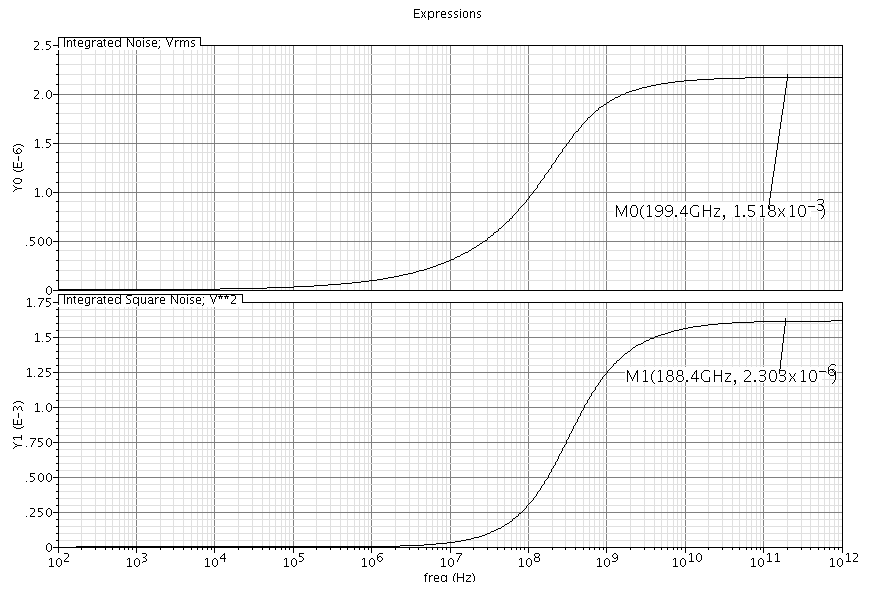
\includegraphics[width=\textwidth]{acsamplenoisediff}
\caption{AC Noise During Sampling Phase of Differential ADC} 
\label{fig:acsamplenoisediff}
\end{figure}
\begin{figure}[htbp]
\centering
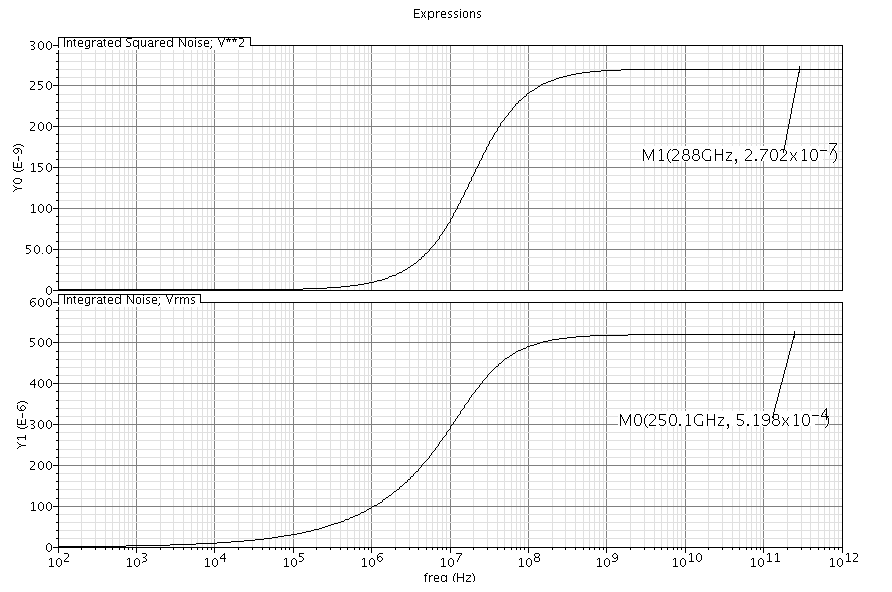
\includegraphics[width=\textwidth]{acholdnoisediff}
\caption{AC Noise During Amplification Phase of Differential ADC} 
\label{fig:acholdnoisediff}
\end{figure}
Not surprisingly, the noise contribution from the sampling phase has roughly doubled. This is due to the doubling of the capacitance from the differential design. The noise in the amplification phase does not exactly double because the OTA noise power is independent of the differential or single-ended implementation. The contribution to amplification phase noise power from the input switches and from the second stage capacitive array does double, however. Table \ref{tab:acnoisesummarydiff} summarizes the results from the AC noise simulation.
\begin{table}[htbp]
\begin{center}
\begin{tabularx}{\linewidth}{|l|X|X|X|X|}
\hline
Setup & AC Sampling Noise (\si{\milli\volt_{rms}}) & Total AC Hold Noise  (\si{\milli\volt_{rms}}) & AC Hold OTA Noise  (\si{\milli\volt_{rms}}) & AC Total Noise  (\si{\milli\volt_{rms}}) \\ \hline
Simulation & 1.52 & 0.52 & 0.32 & 1.60 \\ \hline
Calculation & 1.51 & 0.34 & 0.33 & 1.55 \\ \hline
Design Target & 1.51 & 1.62 & 1.51 & 2.21 \\ \hline
Error (\%) & 0.31 & 53.79 & -1.69 & 3.48 \\ \hline
Headroom (\%) & -0.26 & 67.82 & 78.66 & 27.55 \\ \hline
\end{tabularx}
\end{center}
\caption{Differential AC Output Noise Summary}
\label{tab:acnoisesummarydiff}
\end{table}
Once again, the hold noise calculations are off due to neglecting the contribution to noise power of the input switches. Despite this limitation, the noise power is still well within the budget. Figure \ref{fig:pnoisediff} is the result of the PSS/PNOISE simulation with the differential ADC.
\begin{figure}[htbp]
\centering
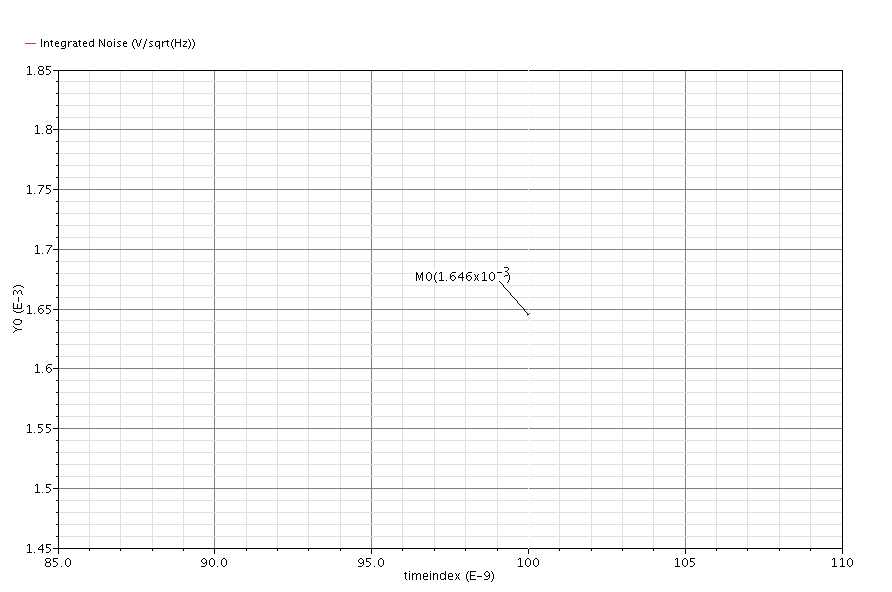
\includegraphics[width=\textwidth]{pnoisediff}
\caption{Differential PNOISE Simulation Result} 
\label{fig:pnoisediff}
\end{figure}
The results from this simulation are compared with the noise calculations and the results from the AC noise simulation in Table \ref{tab:pnoisesummarydiff}. 
\begin{table}[htbp]
\begin{center}
\begin{tabularx}{\linewidth}{|l|X|X|X|}
\hline
Setup & Total Noise Power (\si{\milli\volt_{rms}}) & Error vs Calculation (\%) & Error vs AC Simulation (\%) \\ \hline
PNOISE Simulations & \multicolumn{1}{r|}{1.65} & \multicolumn{1}{r|}{6.21} & \multicolumn{1}{r|}{2.64} \\
\hline
\end{tabularx}
\end{center}
\caption{Differential PNOISE Output Noise Summary}
\label{tab:pnoisesummarydiff}
\end{table}
The differential PNOISE results agreed closely with the calculated results and the AC noise simulations, so the noise simulations were considered successful.

As in the case of the single-ended design, an equivalent SNDR could now be calculated with the SQDR and noise power. The differential PNOISE noise power was used, as this was the largest simulated noise power. The calculated SNDR for the differential design was:
\begin{equation}
\label{eq:sndridealdiff}
SNDR = \SI{72.6}{\decibel}
\end{equation}
From Equation \ref{eq:sndridealdiff}, the ENOB is calculated to be 11.8 bits, which is better than the result from the single-ended design. With the differential ADC design performance meeting specification, the design could move on to the next phase, implementing transistor-level designs for the OTA.
\chapter{MDAC Design and Integration}
After successfully simulating the design with ideal circuit blocks, the next step was to perform the transistor level design of the MDAC. The MDAC is one of the most important blocks in a pipelined ADC design. The accuracy of the closed-loop gain directly affects the accuracy of the downstream ADC. In addition, the overall power consumption and noise power is generally dominated by the contributions from the MDAC, so careful design of the MDAC is required in order to obtain high accuracy and low power consumption. From Section \ref{sec:mdacoperation}, the MDAC consists of an OTA along with a capacitive feedback network. Since the feedback network and OTA parameters had already been specified in Section \ref{sec:designparameters}, the main design task was to meet the required specifications using a transistor level design. This chapter will begin with a discussion of the chosen OTA architecture, as well as the main design knobs used to obtain the required OTA specifications. Next will be a high level overview of the biasing and CMFB networks used to obtain the OTA operating point. Following this is a discussion of the simulation methods used and some design challenges that had to be overcome after initial simulations. This chapter then moves on to a presentation of the simulation results of the OTA. Finally, the performance results of the full ADC with the OTA integrated are presented and a final FOM of the design is calculated.
\section{OTA Design}
From Section, \ref{sec:idealotaparams}, in order to achieve the required static and dynamic errors, a loop gain of \SI{48}{\decibel} and a loop crossover frequency of \SI{22.1}{\mega\hertz} was required. The main factor driving the choice of OTA topology was the large gain required. The maximum gain in almost all OTA architectures is set by the intrinsic gain, \gmgds\spc or \gmro, of its transistors. In order to achieve an open-loop gain of \SI{73}{\decibel} using a topology with a gain of approximately $(g_mr_o)^2$, an intrinsic gain of approximately \SI{36}{\decibel} would be required. Assuming minimum channel length devices, intrinsic gains this large would not be achievable. If, however, a topology with a gain of approximately $(g_mr_o)^3$ was used, the required intrinsic gain drops to approximately 16. An intrinsic gain of 16 is attainable using minimum channel length devices, so the investigation was limited to topologies with a gain proportional to $(g_mr_o)^3$. Two topologies that fit this requirement are a triple cascoded topology and a two-stage topology with a cascoded first stage. In general, two stage designs require pole splitting to maintain stability, which causes the dominant pole to shift lower. These concerns are not present with cascoded designs, since the nondominant pole is generally close to the transit frequency. This means that higher bandwidths are easier to obtain using a single triple cascoded stage. In addition, using a single stage generally consumes less power, since each stage requires its own bias current. The main reason why many designs do not use a triple cascoded topology is their extremely limited output swing. For a triple cascoded differential topology, the output voltage range is approximately:
\begin{equation}
\label{eq:triplecascodeoutputswing}
-(V_{dd} - 7V_{ov}) < V_{out} < (V_{dd} - 7V_{ov})
\end{equation}
where $V_{ov}$ is the overdrive voltage of the transistors. For many low-voltage processes, this limitation prohibits the usage of this topology.

In this design the usage of the half-gain topology allows for the usage of the triple-cascode topology. The half-gain topology reduces the maximum output swing of the second stage to \SI{1}{\volt}, assuming a comparator offset of $\nicefrac{1}{2}$ LSB. Using a \SI{1.8}{\volt} supply and assuming an overdrive voltage of approximately \SI{200}{\milli\volt}, the maximum output swing would be approximately \SI{1.2}{\volt}, which is large enough to meet the needs for this design. This fact, along with the many advantages of using a single stage topology, drove the decision to use this architecture. The other major disadvantage of this architecture is the complex biasing required to maintain proper bias voltages on the five transistors in the stack, but since this would only mean more design effort, this did not affect the choice to use this architecture. Figure \ref{fig:triplecascode} shows a general triple cascode OTA. 
\begin{figure}[htbp]
\newcommand{\colspacing}{3}
\newcommand{\rowspacing}{-2}
\newcommand{\rowone}{0}
\newcommand{\rowtwo}{\rowone+\rowspacing}
\newcommand{\rowthree}{\rowtwo+\rowspacing}
\newcommand{\colone}{0}
\newcommand{\coltwo}{\colone+\colspacing}
\centering
\begin{circuitikz} 
\draw
%First pmos transistor in the stack
(\colone,\rowtwo) node[pmos, xscale=-1] (mp1l) {}
(\coltwo,\rowtwo) node[pmos] (mp1r) {}
%Vdd connection
(mp1l.S) -- node[anchor=south] (vdd) {$V_{dd}$} (mp1r.S)
%Vb1 connection
(mp1l.G) -- node[anchor=south] (vb1) {$V_{b1}$} (mp1r.G)
%Second pmos in the stack
(mp1l.D) node[pmos, anchor=S, xscale=-1] (mp2l) {}
(mp1r.D) node[pmos, anchor=S] (mp2r) {}
%Vb2 connection
(mp2l.G) -- node[anchor=south] (vb2) {$V_{b2}$} (mp2r.G)
%Third pmos in the stack
(mp2l.D) node[pmos, anchor=S, xscale=-1] (mp3l) {}
(mp2r.D) node[pmos, anchor=S] (mp3r) {}
%Vb3 connection
(mp3l.G) -- node[anchor=south] (vb3) {$V_{b3}$} (mp3r.G)
%Output node
(mp3l.D) -- ++(-0.5, 0) node[anchor=east] (voutn) {$V_{outn}$} 
(mp3r.D) -- ++(0.5, 0) node[anchor=west] (voutp) {$V_{outp}$} 
%First nmos in stack
(mp3l.D) node[nmos, anchor=D, xscale=-1] (mn1l) {}
(mp3r.D) node[nmos, anchor=D] (mn1r) {}
%Vb4 connection
(mn1l.G) -- node[anchor=south] (vb4) {$V_{b4}$} (mn1r.G)
%Second nmos in stack
(mn1l.S) node[nmos, anchor=D, xscale=-1] (mn2l) {}
(mn1r.S) node[nmos, anchor=D] (mn2r) {}
%Vb5 connection
(mn2l.G) -- node[anchor=south] (vb5) {$V_{b5}$} (mn2r.G)
%Input nmos
(mn2l.S) node[nmos, anchor=D] (mn3l) {}
(mn2r.S) node[nmos, anchor=D, xscale=-1] (mn3r) {}
(mn3l.G) node[anchor=east] (vinp) {$V_{inp}$}
(mn3r.G) node[anchor=west] (vinn) {$V_{inn}$}
(mn3r.S) --  (mn3l.S)
% Tail current sources
(mn3l.S) ++(1, 0) node[nmos, anchor=D] (mntail) {}
(mntail.G) node[anchor=east] (vbias) {$V_{currmirr}$}
(mn3r.S) ++(-1, 0) node[nmos, anchor=D, xscale=-1] (mncmc) {}
(mncmc.G) node[anchor=west] (vcmc) {$V_{cmc}$}
% Ground node
(mntail.S) -- node[ground] (gnd) {} (mncmc.S)
;
\end{circuitikz}
\caption{Triple Cascode OTA}
\label{fig:triplecascode}
\end{figure} 
In this design, two equally sized tail transistors were used as the current source. The first had a fixed bias set by a current mirror, with value $V_{currmirr}$. The second had a variable bias used to set the output common-mode to its desired voltage. The output voltage from the CMFB network is denoted in this figure as $V_{cmc}$. The design of the biasing network and the CMFB network is covered in Sections \ref{sec:biasnetwork} and \ref{sec:otacmfb}. The following sections will discuss in more detail the different performance parameters for the triple cascode topology, as well as their relationship to the main design knob, \gmid.
\subsection{Primary OTA Performance Goals}
The three critical OTA design parameters were the loop gain, loop crossover frequency, and output noise power. If these specifications were not met, the ADC would not perform within its accuracy specifications.
\subsubsection{OTA Loop Gain}
From Equation \ref{eq:loopgain}, the factors controlling the loop gain of the OTA are the open-loop gain of the OTA and the OTA feedback factor. This section will derive expressions for each of these parameters in terms of device characteristics, and discuss their dependence on \gmid. 

The open-loop gain of the OTA is approximately equal to the product of its effective transconductance, $G_{m}$, and its output resistance, $R_{out}$. For the triple-cascode topology, the signal path consists of a common source transistor followed by two common gate transistors. Since the current gain of the common gate transistors is approximately one, the effective transconductance of this configuration is:
\begin{equation}
\label{eq:gmeffective}
G_{m} = g_{m,CS}
\end{equation}
where $g_{m,CS}$ is the transconductance of the common source transistor. Assuming that the $g_{m}$ of all transistors is equal, a PMOS output resistance of $r_{op}$, and an NMOS output resistance of $r_{on}$, the approximate output resistance of this configuration is:
\begin{equation}
\label{eq:triplecascodero}
R_{out} \approx (g_{m}^{2}r_{on}^{3}) || (g_{m}^2r_{op}^{3})
\end{equation}
The expression for the open-loop gain of this configuration is:
\begin{equation}
\label{eq:triplecascodegain}
A_{OLDC} = G_{m}R_{out} \approx \dfrac{(g_{m}r_{o})^{3}}{2}
\end{equation}
where this expression assumes that the output resistance of the PMOS and NMOS transistors is approximately equal. From this equation, it can be seen that maximizing \gmgds\spc will also maximize the open-loop gain of the amplifier. Since $g_{ds}$ is directly proportional to $I_{d}$, a larger \gmid\spc implies a higher \gmgds, which means a larger gain.

Up until this point, a simplified model for the feedback factor has been used. This model only accounted for the effect of the MDAC feedback capacitor and first stage sampling capacitors on the feedback factor. A more accurate model incorporating the effect of the amplifier input capacitance, $C_{in}$ is:
\begin{equation}
\label{eq:accuratebeta}
\beta = \dfrac{C_{f}}{C_{f}+C_{s1}+C_{in}}
\end{equation}
The input capacitance of the amplifier is a function of the parasitic capacitance from the input NMOS transistor. An approximate expression for the input capacitance in terms of the input NMOS device parasitics is:
\begin{equation}
\label{eq:ampinputcap}
C_{in} = C_{gs} + 2C_{gd}
\end{equation}
where $C_{gs}$ is the gate to source capacitance and $C_{gd}$ is the gate to drain capacitance. The factor of two applied to $C_{gd}$ comes from the application of the Miller approximation to a cascoded common source stage. From Equations \ref{eq:accuratebeta} and \ref{eq:ampinputcap}, larger device parasitics will degrade the feedback factor. From Section \ref{sec:gmid}, a larger \gmid\spc generally means larger device parasitics. From this the tradeoff between increased open-loop gain and decreased feedback factor can be seen. This tradeoff becomes even more important when the OTA loop crossover frequency.
\subsubsection{OTA Loop Crossover Frequency}
From Equation \ref{eq:fc}, the OTA loop crossover frequency is dependent upon the feedback factor, the OTA transconductance, and the total load capacitance. Up to this point, Equation \ref{eq:cltotapprox} has been used when estimating the load capacitance. A more accurate equation for load capacitance that accounts for the parasitic capacitances from the PMOS and NMOS transistors connected to the output node is:
\begin{equation}
\label{eq:cltotexact}
C_{l,tot} = C_{s2} + (1-\beta)\cdot C_{f} + C_{db,p} + C_{gd,p} + C_{db,n} + C_{gd,n} 
\end{equation}
where $C_{db,p}$ and $C_{db,n}$ are the drain to bulk capacitances for the PMOS and NMOS respectively, and $C_{gd,p}$ and $C_{gd,n}$ are the gate to drain capacitances for the PMOS and NMOS respectively. Here, again, larger \gmid\spc will cause larger device parasitics, which will limit the loop crossover frequency of the OTA. In order to achieve both the gain and crossover frequency goals, \gmid\spc of the load transistors must be carefully chosen to balance the tradeoffs between these two metrics. A degree of freedom is offered by the dependence of loop crossover frequency on \Gm, but care must be taken when using this knob as increased \Gm\spc also means increased power consumption. 
\subsubsection{OTA Noise} 
\label{sec:realotanoise}
From Equation \ref{eq:cascoutputnoise}, the main factors in OTA output noise are the ratio of common gate transconductance to common source transconductance, and the ratio of the loop crossover frequency to the non-dominant pole frequency. Decreasing the common gate to common source transconductance ration implies using a small $g_{m}$, and thus a small \gmid, in the common gate transistors. Due to headroom issues, this ratio had to be kept around 1, so it was decided that the transconductance ratio would not be a knob used to decrease the OTA output noise. Fortunately, more latitude was available in the ratio of the loop crossover frequency to non-dominant pole frequency. In addition to the dominant pole at the output node, there are two additional nodes on the signal path that contribute non-dominant poles. Assuming that all transistors on the signal path are sized equally, the capacitance at each node, $C_{x}$, will be:
\begin{equation}
\label{eq:nondominantcap}
C_{x} = C_{gd,n} + C_{gs,n} + C_{sb,n} + C_{db,n}
\end{equation}
where $C_{sb,n}$ is the source to bulk capacitance of the NMOS transistor. The resistance, $R_{x}$ at each of these nodes is essentially the input resistance of a common gate transistor, which is:
\begin{equation}
\label{eq:nondominantres}
R_{x} = \dfrac{1}{g_{m}}
\end{equation}
Using the expressions from Equations \ref{eq:nondominantcap} and \ref{eq:nondominantres}, the non-dominant pole frequencies, $\omega_{p2,3}$ are:
\begin{equation}
\omega_{p2,3} = \dfrac{g_{m}}{C_{x}} 
\end{equation}
The ratio between the loop crossover frequency and the non-dominant pole frequencies essentially simplifies to the ratio between the load capacitance and the non-dominant node capacitances. From the data in Table \ref{tab:parcapotagmid}, even for very large \gmid\spc values the total gate capacitance only approaches 10\% of the load capacitance. From this observation, the expected ratio between loop crossover frequency and non-dominant pole frequency could be expected to be much larger than the 3:1 ratio assumed in Section \ref{sec:designparameters}. Even if the expression from Equation \ref{eq:noiseconstexpression} underestimated the actual design noise power, the expectation was that the noise power should not exceed the specified limits. For this reason, noise power was not given much consideration in the overall amplifier design. If necessary, the common gate transistors' $g_{m}$ and \transit\spc could be tweaked once other design specifications were met, but the assumption that this likely would not be an issue was made.
\subsection{Secondary Design Goals}
Beyond the specifications required to meet the stated ADC performance specifications, some additional design parameters were accounted for in the design phase. Maximizing the output swing would allow for larger first-stage comparator offsets without compromising the accuracy of the ADC. Obtaining a phase margin larger than the minimum required $45^{\circ}$ provides better settling performance. Finally, the power consumption of the OTA is typically the dominant contributor to pipelined ADC power consumption, so reducing power consumption as much as possible was crucial to obtaining maximum ADC power effficiency. This section will provide an overview of the design parameters affecting these secondary design goals. 
\subsubsection{Output Swing}
Output swing can be a fairly ambiguous term, for the purposes of this design the output swing is defined as the output voltage points where the open-loop gain degrades 30\% from its peak value. In order for the ADC to meet its accuracy specifications, the absolute minimum output swing is \SI{0.5}{\volt}. Having an output swing of only \SI{0.5}{\volt}, however, constrains the maximum comparator offset to zero. In real comparator implementations, this constraint would be unrealistic. In order for the design to be able to take full advantage of the 1-bit redundancy, allowing for a maximum comparator offset of $\nicefrac{1}{2}$ LSB, the output swing of the OTA must be \SI{1}{\volt}. Anything between these two values will constrain the comparator offset to below the value allowed for by the redundancy scheme. Using Equations \ref{eq:triplecascodeoutputswing} and \ref{eq:vov} with a targeted output swing of \SI{1}{\volt} and assuming that the \gmid\spc of all transistors is the same, the minimum \gmid\spc is:
\begin{align}
\label{eq:gmidoutputswing}
(g_{m}/I_{d})_{min} &= \dfrac{28}{2\cdot V_{dd} - 1} \\[0.5em]
\nonu				&= 10.8
\end{align}
In order to ensure maximum allowable comparator offset, the \gmid\spc was maintained above this value.
\subsubsection{Phase Margin}
The same concerns from Section \ref{sec:realotanoise} apply to phase margin, since the ratio between the loop crossover frequency and the non-dominant pole frequencies determine the phase margin. From the analysis in the OTA noise section, phase margin was expected to be well above the 3:1 value needed to obtain the desired settling behavior, so this design criteria was largely ignored in the design phase. In the case of loop gain simulations that showed instability, the size of the common-gate transistors could be reduced in order to reduce capacitance at the non-output nodes.
\subsubsection{Power Consumption}
The OTA power consumption is dependent on the supply voltage and the bias current. Assuming a fixed supply voltage of \SI{1.8}{\volt}, minimizing bias current is the only knob to reduce power consumption. Required bias current is a function of both the \gmid\spc and the $g_{m}$ of the design. Larger \gmid\spc means that for a given transconductance, the bias current will be lower. Larger \gmid\spc also implies a lowered \transit, however, which implies a larger required transconductance in order to meet bandwidth requirements. Some design iteration is generally required to find the optimal combination of \gmid\spc and $g_{m}$ to minimize power consumption.
\subsection{Initial Design Parameters}
After analyzing all the design goals and their various tradeoffs, an initial design could be specified. A Matlab script was created in order to calculate the bias current and transistor widths required to meet the OTA specifications. The only constraint given to this script was the design \gmid. In this way, various \gmid\spc values could be specified and its effect on different transistor parameters could be observed. A limitation of this script was that it assumed the \gmid\spc of all design transistors was the same, but for the purposes of a first pass design this limitation was deemed acceptable. The purpose of this design script was a) to obtain a solution that was close to optimal, and b) to use the knowledge gained from the analysis of the design to make small manual changes to the transistor parameters, and then re-simulate. After some experimentation, a \gmid\spc of 15 was settled upon for the transistors. A summary of the major design parameters, along with some estimated performance parameters, is given in Table \ref{tab:firstpassotadesign}. 
\begin{table}[htbp]
\begin{center}
\begin{tabular}{|l|r|}
\hline
Parameter & \multicolumn{1}{l|}{Value} \\ \hline
$g_{m}/I_{d}$ & \SI{15}{\per\volt} \\ \hline
$V_{ov}$ & \SI{.13}{\volt} \\ \hline
$g_{m}$ & \SI{3.41}{\milli\siemens} \\ \hline
$I_{total}$ & \SI{454}{\micro\ampere} \\ \hline
$W_{PMOS}$ & \SI{124}{\micro\meter} \\ \hline
$W_{NMOS}$ & \SI{24.2}{\micro\meter} \\ \hline
$(g_{m}/g_{ds})_{PMOS}$ & 42.2 \\ \hline
$(g_{m}/g_{ds})_{NMOS}$ & 37.9 \\ \hline
$f_{t,PMOS}$ & \SI{5.73}{\giga\hertz} \\ \hline
$f_{t,NMOS}$ & \SI{16.2}{\giga\hertz} \\ \hline
$A_{oldc}$ & \SI{90}{\decibel} \\ \hline
Loop gain & \SI{65}{\decibel} \\ \hline
$f_{c}$ & \SI{23}{\mega\hertz} \\ \hline
Phase Margin & \SI{89.9}{\degree} \\ \hline
\end{tabular}
\caption{Initial OTA Design Parameters}
\label{tab:firstpassotadesign}
\end{center}
\end{table}
With these base design specifications, the only tasks left before running simulations were designing the bias network and the CMFB network.
\section{Bias Network Design}
\label{sec:biasnetwork}
A carefully designed bias network was crucial to ensure maximum output swing and acceptable common-mode rejection. In order to maximize output swing, the bias network had to ensure that the bias voltage on each of the non-input transistors would produce a $V_{DS}$ that was on the edge of saturation. A poorly designed bias network could obtain the required performance specifications while significantly degrading the output swing of the OTA. In order to maximize common-mode rejection, the tail current mirror had to be designed properly. This section discusses the design of both the non-input transistor bias and the tail current mirror.
\subsection{Biasing Cascoded Transistors}
\label{sec:cascodebias}
Special design techniques are required to ensure that the bias voltages of the transistors produce a $V_{DS}$ on the edge of saturation. Figure \ref{fig:biasnetworkvdscontrol} illustrates how the biasing network can ensure that the $V_{DS}$ of each transistor in the cascode stack is on the edge of saturation.
\begin{figure}[htbp]
\centering
\begin{circuitikz}
\draw
(0,0) node[nmos] (mn1) {MN1}
(mn1.G) node[anchor=east] (vb1) {$V_{b1}$}
(mn1.S) ++(0,-1.5) node[nmos] (mn0) {MN0}
(mn0.D) -- (mn1.S)
(mn0.G) node[anchor=east] (vb0) {$V_{t} + V_{ov}$}
(mn1.S) ++(0, -.25) to [short, *-] ++(-0.25,0) node[anchor=east] (vx) {$V_{x}$}
;
\end{circuitikz}
\caption{Simplified Cascode Stack}
\label{fig:biasnetworkvdscontrol}
\end{figure} 
For the purposes of this example, the desired overdrive voltage on both MN0 and MN1 is assumed to be equal to $V_{ov}$. The minimum voltage at $V_{x}$ for MN0 to remain in saturation is:
\begin{equation}
\label{eq:vdsminbias}
V_{x,min} = V_{ov}
\end{equation}
In order for the overdrive voltage of transistor MN1 to be $V_{ov}$, $V_{x}$ must be:
\begin{equation}
\label{eq:vdsvb1}
V_{x} = V_{b1} - V_{ov}
\end{equation}
In order to bias MN1 to the desired overdrive voltage, while also maintaining the minimum voltage at $V_{x}$, $V_{b1}$ must be:
\begin{equation}
\label{eq:vb1min}
V_{b1,min} = V_{t} + 2V_{ov}
\end{equation}
Any value of $V_{b1}$ larger than this will result in a non-optimal output swing. A similar analysis could be performed on a three transistor stack to show that the optimal bias voltage for the third transistor is $V_{t}+3V_{ov}$.
A number of circuit implementations that meet the requirements of Equation \ref{eq:vb1min} are covered in \cite{bok:gray}. From these, an implementation using a diode-connected transistor in series with a triode transistor was chosen. Figure \ref{fig:highswingbias} illustrates this configuration.  
\begin{figure}[htbp]
\centering
\begin{circuitikz}
\draw
(0,0) -- node[anchor=south] (vdd) {$V_{dd}$} (0.5, 0)
(0.25, 0) -- (0.25, -0.5) to[I=$I_{in}$] (0.25, -1.25)
to [short] (0.25, -2.25) ++(0, -.25) node[nmos] (mn2) {MN2}
(mn2.S) -- ++(0, -0.5) ++(0,-0.25) node[nmos] (mn3) {MN3}
(mn3.G) -- (mn2.G)
(mn2.G) |- node[anchor=south] (vb1) {$V_{b1}$}(mn2.D)
(mn3.S) node[ground] (gnd) {}
;
\end{circuitikz}
\caption{High Swing Bias Configuration}
\label{fig:highswingbias}
\end{figure} 
MN2 operates in the saturation region and MN3 operates in the triode region. From the figure, the value of $V_{b1}$ is equal to the gate to source voltage of MN3. The current through both MN2 and MN3 is equal to $I_{in}$, so the expression for the current in terms of the transistor parameters for MN2 and MN3 is:
\begin{equation}
\label{eq:iinbias}
\dfrac{k^{'}}{2}\left(\dfrac{W}{L}\right)_{2}(V_{gs2} - V_{t})^2 = \dfrac{k^{'}}{2}\left(\dfrac{W}{L}\right)_{3}\left(2(V_{gs3} - V_{t})V_{ds3}-V_{ds3}^2\right)
\end{equation}
In order to satisfy Equation \ref{eq:vb1min}, the drain to source voltage of MN3 must be:
\begin{equation}
\label{eq:vds3bias}
V_{ds3} = V_{ov}
\end{equation}
when
\begin{equation}
\label{eq:vgs2bias}
V_{gs2} = V_{t}+V_{ov}
\end{equation}
If these conditions holsd true, the expression for $V_{b1}$ will be:
\begin{align}
\label{eq:vb1bias}
V_{b1} &= V_{gs3} \\
\nonu  &= V_{gs2} + V_{ds3} \\
\nonu	   &= V_{t} + 2V_{ov} 
\end{align}
This expression matches that from Equation \ref{eq:vb1min}. Using Equations \ref{eq:iinbias}, \ref{eq:vds3bias}, \ref{eq:vgs2bias}, and \ref{eq:vb1bias}, and solving for the relationships between the aspect ratios of MN2 and MN3:
\begin{equation}
\left(\dfrac{W}{L}\right)_{3} = \dfrac{1}{3}\left(\dfrac{W}{L}\right)_{2}
\end{equation}

Using the biasing circuit from Figure \ref{fig:highswingbias} the full triple-cascoded biasing circuit could be designed. For the third transistor in the cascode stack, a gate voltage of $V_{t} + 3V_{ov}$ is desired. Following a similar analysis as in the derivation for the second transistor biasing, the ratio of MN2 to MN3 aspect ratio is 8:1. An important note is that in order to increase the bias voltage, the ratio of MN2 to MN3 aspect ratio must be increased. These results were used to design the full bias circuit shown in Figure \ref{fig:fullbias}.
\begin{figure}[htbp]
\centering
\newcommand{\colspacing}{5}
\newcommand{\rowspacing}{-2}
\newcommand{\rowone}{0}
\newcommand{\rowtwo}{\rowone+\rowspacing}
\newcommand{\rowthree}{\rowtwo+\rowspacing}
\newcommand{\colone}{0}
\newcommand{\coltwo}{\colone+\colspacing}
\begin{circuitikz}
\draw
% Third cascode stack bias
(0,0) -- node[anchor=south] (vdd) {$V_{dd}$} (0.5, 0)
(0.25, 0) -- (0.25, -0.5) to[I=$I_{in}$] (0.25, -1.25)
to [short] (0.25, -2.25) ++(0, -.25) node[nmos] (mn1) {MN1}
(mn1.S) node[anchor=west] (wl2) {$\dfrac{W}{L}$}
(mn1.S) -- ++(0, -1) node[nmos, anchor=D] (mn2) {MN2}
(mn2.S) node[anchor=west] (wl3) {$\dfrac{1}{8}\left(\dfrac{W}{L}\right)$}
(mn2.G) -- (mn1.G) to [short, -*] ++(0, 0) 
(mn1.D) ++(0, 0.25) to [short, -*] ++(0, 0) -| node[anchor=south] (vb4) {$V_{b4}$}(mn1.G)
(mn2.S)-- ++(0, -0.5) node[ground] (gnd) {}
% Second Cascode stack bias
(\coltwo,0) -- node[anchor=south] (vdd) {$V_{dd}$} ++(0.5, 0)
(\coltwo+0.25, 0) -- (\coltwo+0.25, -0.5) to[I=$I_{in}$] (\coltwo+0.25, -1.25)
to [short] (\coltwo+0.25, -2.25) ++(0, -.25)
node[nmos] (mn3) {MN3}
(mn1.D) ++(0, 0.25) -- ++(1.5, 0) |- (mn3.G)
(mn3.S) node[anchor=west] (wl3) {$\dfrac{W}{L}$}
(mn3.S) -- ++(0, -1) node[nmos, anchor=D] (mn4) {MN4}
(mn4.S) node[anchor=west] (wl4) {$\dfrac{W}{L}$}
(mn4.S) -- ++(0, -1) node[nmos, anchor=D] (mn5) {MN5}
(mn5.S) node[anchor=west] (wl5) {$\dfrac{1}{3}\left(\dfrac{W}{L}\right)$}
(mn5.G) -- ++(-0.5, 0) |- (mn4.G)
(mn4.G) -- ++(-0.5, 0) to [short, -*] ++(0, 0) |- node[anchor=south] (vb5) {$V_{b5}$}(mn3.D) to [short, -*] ++(0, 0)
(mn5.S) -- ++(0, -0.5) node[ground] (gnd) {}
;
\end{circuitikz}
\caption{Full Cascode Bias Circuit}
\label{fig:fullbias}
\end{figure}
$V_{b4}$ and $V_{b5}$ correspond to the bias voltage connections in Figure \ref{fig:triplecascode}. The addition of MN3 is necessary in order to maintain the same $V_{ds}$ values for MN5 and the second cascode transistor in the triple cascode topology. Maintaining equal $V_{ds}$ values for these transistors removes systematic gain error of the current mirror~\cite{bok:gray}. A very similar topology was used to bias the PMOS transistors, with an additional transistor stack to bias the PMOS transistor closest to the power supply.
\subsection{Tail Current Source Design}
Designing a tail current source with high output resistance is important in obtaining high common-mode rejection for the OTA. In an effort to maximize the output resistance, many designs use a cascoded current mirror rather than a simple single transistor mirror. However this option did not seem feasible for this design due to the already limited output swing caused by the triple cascode topology. In an effort to increase the output resistance, a non-minimum channel length of \SI{360}{\nano\meter} was used for the tail transistor. In addition, the \gmid\spc was kept high in order to both maintain a large output resistance and to minimize the effect on output swing from the tail transistor.
\section{Common-Mode Feedback Design}
\label{sec:otacmfb}
For differential designs, the operating output voltage is very sensitive to small changes in device characteristics~\cite{315areader}. Small changes in the bias voltage can cause very large changes in the operating output voltage. In order to control these variations, common-mode feedback is employed. Common-mode feedback applies a variable amount of bias current in order to correct for excursions from the ideal output common-mode voltage. In order to achieve this, circuits are required to sense the common-mode voltage, to compare this sensed voltage to the desired common-mode voltage, and to apply a variable amount of current based on the difference between actual output common-mode and desired commmon-mode. For the purposes of initial design simulations, an ideal CMFB network was used to ensure that the base OTA design worked by itself. In later design stages, a real CMFB implementation was implemented and tested. The following sections discusses both the ideal and real CMFB implementations.
\subsection{Ideal CMFB}
Figure \ref{fig:idealcmfb} illustrates the schematic for the ideal CMFB network. 
\begin{figure}[htbp]
\centering
\begin{circuitikz}
\draw
(0,0) node[transformer] (t1) {}
(t1.A2) ++(0,-0.5) node[transformer, anchor=A1] (t2) {}
(t1.A2) -- node[anchor=east] (vcm) {$V_{cmo}$} (t2.A1)
(t1.A1) node[anchor=east] (vop) {$V_{op}$}
(t2.A2) node[anchor=east] (vom) {$V_{om}$}
(t1.B2) -- ++(0.5, 0) |- (t2.B2)
(t2.B1) -| (t1.B1)
(t1.B1) node[anchor=west] (vdmo) {$V_{dmo}$}
(t2.B2) node[ground] (gnd) {}
(3,0) node[anchor=south] (iout) {$I_{out}$} to [cI=$A_{v}\cdot(V_{cm,desired}-V_{cmo})$] (3,-2)
node [ground] (gnd) {}
;
\end{circuitikz}
\caption{Ideal CMFB}
\label{fig:idealcmfb}
\end{figure} 
$V_{op}$ and $V_{om}$ are the positive and negative output voltages, respectively. An ideal balun is used as the sensing element to separate the common-mode, $V_{cmo}$, and differential-mode, $V_{dmo}$, voltages from the output signal. The transistor with variable bias in Figure \ref{fig:triplecascode} is replaced with the voltage controlled current source in Figure \ref{fig:idealcmfb}. This current source performs both the comparison as well as current application functions described earlier. When the gain of the controlled source, $A_{v}$, is set to be very large, the output common-mode voltage will be very close to the desired common-mode voltage, which is the desired operation of the CMFB network.
\subsection{Real CMFB Design}
After performing simulation with the ideal CMFB and ensuring that all of the desired OTA specifications were met, a real CMFB implementation had to be designed. The simplest method to sense the output common-mode voltage is to use a resistive divider. The issue with using resistors on the output is that they have to be very large to not destroy the differential gain of the amplifier. This issue can be overcome by buffering the output with source followers, but this causes headroom issues. A simpler solution to the sensing problem is to use purely capacitive sensing. Once the sensing implementation had been decided on, the next step was to decide on the implementation of the comparison and variable current output functions. Many solutions use a similar idea as that used in the ideal CMFB case, by using a voltage controlled current source with high transconductance and applying the output current to the tail of the OTA. This function can be implemented using standard differential transsistor amplification techniques, since MOSFETs in saturation act as voltage controlled current sources. The downside to applying this strategy is the additional bias current required to implement an additional differential amplifier. This additional bias current can be a large percentage of the current used to bias the main OTA circuit. 

Alternative implementations were investigated since power efficiency was a primary goal in this design. Since this OTA is only required to be active during the second clock phase, a passive CMFB implementation could be used~\cite{315areader}. This implementation still requires additional bias current, but in general the additional current is smaller than in other implementations. Figure \ref{fig:realcmfb} shows a general model for the passive CMFB network.  
\begin{figure}[htbp]
\newcommand{\colspacing}{2}
\newcommand{\rowspacing}{-2}
\newcommand{\rowone}{0}
\newcommand{\rowtwo}{\rowone+\rowspacing}
\newcommand{\rowthree}{\rowtwo+\rowspacing}
\newcommand{\rowfour}{\rowthree+\rowspacing}
\newcommand{\colone}{0}
\newcommand{\coltwo}{\colone+\colspacing}
\newcommand{\colthree}{\coltwo+\colspacing}
\newcommand{\colfour}{\colthree+\colspacing}
\newcommand{\colfive}{\colfour+\colspacing}
\newcommand{\colsix}{\colfive+1+\colspacing}
\centering
\begin{circuitikz} 
\draw
% Input phi2 switches
(\colone, \rowone) node[anchor=east] (vop) {$V_{op}$} to [cspst, l=$\phi_{2}$] (\coltwo, \rowone)
(\colone, \rowtwo) node[anchor=east] (vom) {$V_{om}$} to [cspst, l=$\phi_{2}$] (\coltwo, \rowtwo)
% CMFB caps
(\coltwo, \rowone) -- (\colthree, \rowone) to [short, *-] (\colthree, \rowtwo) to [C, l_=$C_{cmfb}$] (\colthree, \rowthree) to [short, -*] ++(0, 0.38*\rowspacing)
(\coltwo, \rowtwo) -- (\colfour, \rowtwo) to [short, *-] (\colfour, \rowtwo) to [C, l=$C_{cmfb}$] (\colfour, \rowthree) to [short, -*] ++(0, 0.38*\rowspacing)
% Voc,desired
(\colthree, \rowone) -- (\colfour, \rowone) to [cspst, l=$\phi_{1}$] (\colfive, \rowone)
(\colfour, \rowtwo) to [cspst, l=$\phi_{1}$] (\colfive, \rowtwo)
(\colfive, \rowone) --  (\colfive, \rowtwo)
(\colfive, \rowone) ++(0, \rowspacing/2) -- ++(0.5, 0) node[anchor=west] (vocdesired) {$V_{oc,desired}$}
% Bias current
(\colsix,\rowone) ++(-0.25, 0) -- node[anchor=south] (vdd) {$V_{dd}$} ++(0.5, 0)
(\colsix,\rowone) to [I=$0.25I_{tail}$] (\colsix, \rowtwo) -- (\colsix, \rowthree)
% Bias nmos
node[nmos, anchor=D] (mnbias) {}
(mnbias.S) node[ground] (gnd) {}
(mnbias.G) |- (mnbias.D) 
(mnbias.G) node[anchor=south east] (vb) {$V_{b}$}
% Final row switches and connections
(mnbias.G) to [cspst, l=$\phi_{1}$] ++(-\colspacing, 0)
-- ++(-2*\colspacing, 0) node[anchor=east] (vcmc) {$V_{cmc}$}
(\colthree, \rowthree) -- ++(0, 0.4*\rowspacing)
(\colfour, \rowthree) -- ++(0, 0.4*\rowspacing)
;
\end{circuitikz}
\caption{Real CMFB Implementation}
\label{fig:realcmfb}
\end{figure}
In the $\phi_{1}$ clock phase, the voltage across the feedback capacitors, $V_{Ccmfb}$ is charged to:
\begin{equation}
V_{Ccmfb} = V_{oc,desired} - V_{b}
\end{equation}
This charging phase is the reason why the OTA cannot be active during $\phi_{1}$. Once the OTA enters its active phase, $\phi_{2}$, the feedback network will be activated. In this configuration, if the output common-mode is larger than the desired output common-mode, $V_{cmc}$ will become larger than $V_{b}$, which will cause more current to flow through the transistor tail. This additional current will cause the common mode output decrease. The opposite effect occurs if the output common-mode is smaller than the desired output common-mode. The transistor that sets $V_{b}$ is sized to be half of the tail transistor that it controls in order to allow for the bias current to be \nicefrac{1}{4} of the total bias current. An optimization applied to this design was the removal of the additional bias current and bias transistor. Since an appropriate $V_{b}$ was already being generated from the tail current mirror, the output bias voltage from the current mirror could be applied to the CMFB as well. This removed the need for any additional bias current to be applied to the CMFB network. 

Another design consideration is the sizing of the feedback capacitors. These must be sized large enough so that the bandwidth of the common-mode feedback is not so large as to cause instability, but also not too large that the feedback network cannot respond quickly enough to changes in the output common-mode. A good rule of thumb is to make the common-mode feedback bandwidth about 30\% of the differential bandwidth. Assuming that the circuit has approximately 10 time constants to settle, this allows 3 time constants for the CMFB voltage to settle, which can remove approximately 95\% of common-mode disturbance~\cite{315areader}.
\section{OTA Test Setup}
\label{sec:otatests}
In order to ensure that the OTA met its specifications, a number of different simulations had to be run. This section gives a brief overview of the different test setups used to obtain different device parameters. Once all of these simulations produced adequate results, the same simulation as outlined in Section \ref{sec:adcsimulations} were run on the entire ADC with the real OTA model instead of the ideal one.
\subsection{Loop Gain, Loop Crossover Frequency, Phase Margin, and Power Consumption Simulation}
\label{sec:loopsimulation}
A typical method for simulating the loop gain and loop crossover frequency is simulating the OTA in its open loop configuration. The requirements for the open-loop gain can be derived from the loop gain requirements, as done in Equation \ref{eq:otagain}. Similarly, the desired open-loop unity gain frequency can be estimated by dividing the desired loop crossover frequency by the feedback factor, $\beta$. The limitation of simulating with this technique is that it does not take into account the effect of the feedback network on the OTA performance. The feedback capacitor adds additional capacitance at the load, which means open-loop simulations will overestimate the true loop crossover frequency. The additional capacitance can be calculated accurately and added to the load capacitance, so this is not typically an issue in open loop simulations. An issue that is not as easily solved is the degradation of the feedback factor due to the input capacitance of the OTA. Open loop simulations cannot account for this effect, which means that both the loop gain and loop crossover frequency will be overestimated. 

Fortunately, the simulator used in this design offered a method for simulating the performance of the OTA with the feedback network implemented. In order to perform this simulation a special probe was placed in order to break the feedback loop. A special simulation, called an \textit{stb} simulation was performed, which can give information on both the common-mode and differential-mode loop gain and loop crossover frequencies. In addition, this simulation provides the phase margin for the circuit. As a side effect of this simulation, if an operating point is saved, the power consumption of the OTA can also be measured. Unfortunately, the version of the tool used for this design did not have a periodic version of the \textit{stb} analysis available, so these simulations could only be performed on the OTA with ideal CMFB network. Transient simulation were used to validate the settling behavior of the OTA with real CMFB as well as the settling of the output common-mode voltage.
\subsection{Output Swing Simulation}
In order to simulate the output swing, a DC simulation was performed. In this case, the open-loop configuration was used for the OTA. Input DC values were applied that would cause the output voltage to vary across the entire desired differential output swing. The negative and positive output voltages which caused a 30\% decrease in the open-loop gain were recorded, and the difference between these two values were considered to be the output swing.
\subsection{OTA Noise}
Before performing the noise simulations on the entire design, the noise contribution from just the OTA was simulated. A similar setup as that in Section \ref{sec:loopsimulation} was used, where the OTA was placed in its final feedback configuration, and the output AC noise was simulated. This setup is very similar to that of the AC hold noise simulation described in Section \ref{sec:acnoisesim}, except that the switches were not included in this setup. As long as the OTA noise was within the maximum value allowed for in Table \ref{tab:maxoutputnoise}, it was very likely that the overall ADC would meet its noise specifications.
\section{OTA Design Challenges}
After calculating initial design parameters that were expected to meet the specifications, designing the bias network and the CMFB network, and determining the necessary simulations to checkout the design, initial simulations could be run. A number of issues were found in the initial simulations that had to be corrected before obtaining an acceptable result. This section will outline some of the challenges that were encountered and the methods used to overcome them in order to obtain an acceptable design.

The initial loop gain simulation produced a gain significantly below that estimated by the \gmid\spc models. After some investigation, it was discovered that the values for \gmgds\spc and \transit\spc that were estimated by the original \gmid\spc simulations were much higher than the measured results from the simulation. This inaccuracy was due to the dependence of these design parameters on the transistor $V_{ds}$. When creating the device models, the simulations were performed using a constant $V_{ds}$ of \SI{900}{\milli\volt}, with the assumption that the design parameters would not change very much with variation in $V_{ds}$. While this holds true across a wide $V_{ds}$ range, this independence no longer holds with very small values of $V_{ds}$, which was the case with the biasing for this design. After coming to this realization, some additional characterization simulations were performed on the simple NMOS testbench to determine the minimum $V_{ds}$ required to obtain a \transit\spc and \gmgds\spc close to that estimated from the models. Figure \ref{fig:vdsdepgmgds} shows the dependence on $V_{ds}$ of \gmgds\spc and Figure \ref{fig:vdsdeptransit} shows the dependence on $V_{ds}$ of \transit. 
\begin{figure}[htbp]
\centering
\includegraphics[width=\textwidth]{nmosintrinsicgain}
\caption{\gmgds\spc Dependence on $V_{ds}$} 
\label{fig:vdsdepgmgds}
\end{figure}
\begin{figure}[htbp]
\centering
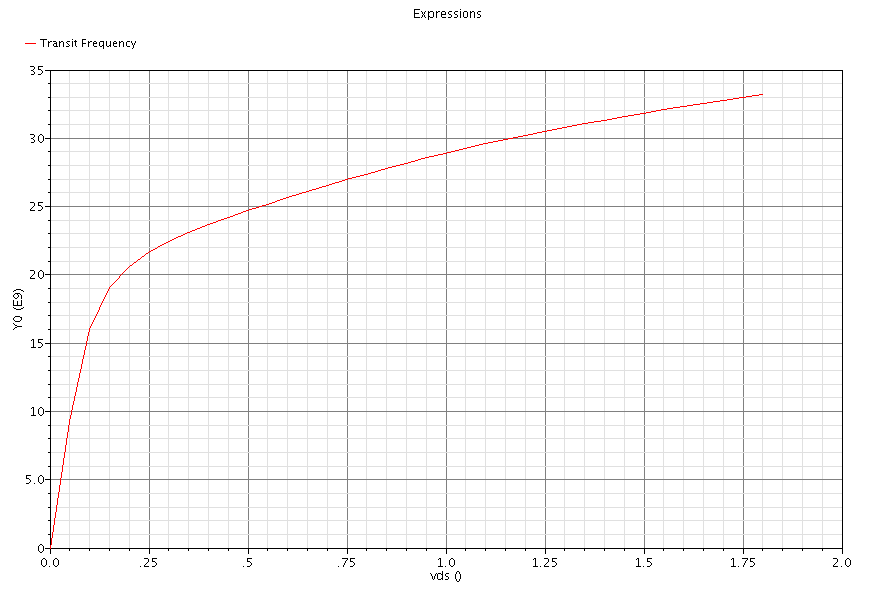
\includegraphics[width=\textwidth]{nmostransitfreq}
\caption{\transit\spc Dependence on $V_{ds}$} 
\label{fig:vdsdeptransit}
\end{figure}
From these graphs, it was decided that the minimum $V_{ds}$ required to obtain results close to the estimated results, while mainataining a reasonable output swing, was \SI{200}{\milli\volt}. In order to achieve this larger transistor drain to source voltage, the method used in Section \ref{sec:cascodebias} was used, to decrease the aspect ratio of the triode transistor. Once all of the transistor $V_{ds}$ voltages were raised to this value, the design parameters began to more closely resemble the calculated models.

Although increasing the $V_{ds}$ on the transistors did increase the gain significantly, this change was not enough for the design to meet the loop gain requirements. In order to increase the gain, the \gmid\spc of the transistors was increased to 20. After making this change, the loop gain specification was met, but the loop crossover frequency was only about \SI{16}{\mega\hertz}, well below the specified requirements. From Equation \ref{eq:cltotexact}, the crossover frequency is only dependent on the parasitics at the load node. In examining the capacitances at the load, it was noticed that the load capacitance contribution from the PMOS was much larger than that from the NMOS. Based on this observation, the width of the load PMOS was reduced in an effort to decrease the load capacitance. A reduction in transistor width while maintaining the same bias current results in a decrease in the transistor \gmid\spc. In the case of the PMOS load, a reduction in \gmid\spc to \SI{15}{\per\volt} was observed. While this modification did increase the crossover frequency of the OTA, it was still not high enough to meet specifications. Further reductions in the load \gmid\spc had little effect on the crossover frequency and caused sharp drops in gain, so the \gmid\spc was not modified any further. In order to meet the required crossover frequency, the $g_{m}$ of all transistors was increased to \SI{4.8}{\milli\siemens}. After this modification, the loop crossover frequency met specification. In retrospect, a much better knob to use would have been the \gmid\spc of the input NMOS transistor. Although the parasitics from the load transistors do reduce the crossover frequency, they are still a small percentage of the second stage sampling capacitance, which dominates the load capacitance. The size of the feedback capacitor is on the same order as the input parasitics, so changes in the input parasitics can have a much larger effect on the feedback factor of the OTA. Unfortunately, this realization was not made until after the design had already been checked out. This optimization will be assessed in future modifications to the OTA.

After overcoming these two major design challenges, the OTA was meeting the loop gain and loop crossover frequency specifications. Further simulations showed that the noise specification was also being met, so the rest of the simulations described in Section \ref{sec:otatests} were performed in order to fully characterize the OTA. The following section will present the results from all of these simulations.
\section{OTA Simulation Results}
This section summarizes the simulation results from the OTA tests described in \ref{sec:otatests}. These results include those from the \textit{stb} analysis, the DC output swing analysis, the AC noise simulation, and the transient simulation used to verify the CMFB network operation. This section will conclude with an overview of device parameters and performance results.
\subsection{STB Results}
The \textit{stb} analysis allowed for loop gain and phase measurements while taking into account the effect of the feedback network on the OTA. Figure \ref{fig:otastbresult} shows the results from this analysis. 
\begin{figure}[htbp]
\centering
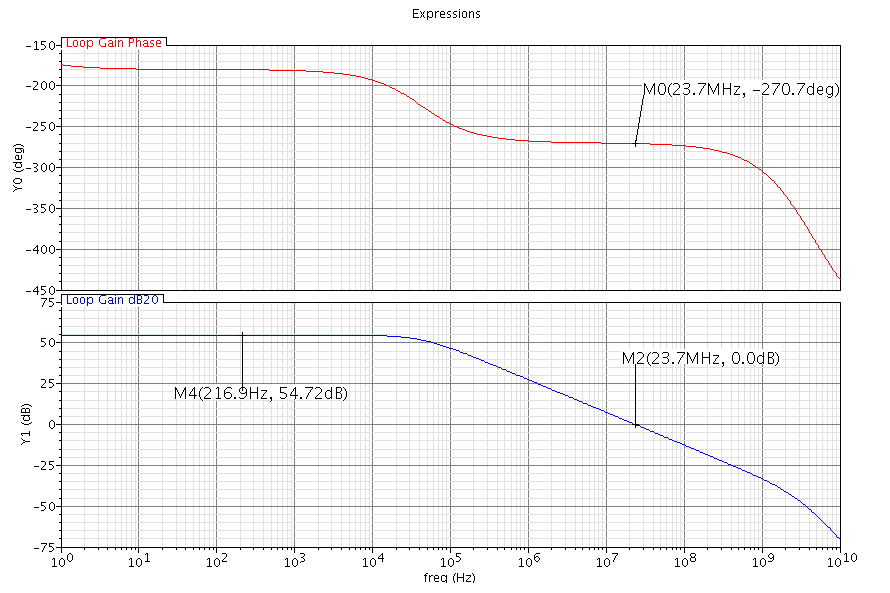
\includegraphics[width=\textwidth]{OTAloopgain}
\caption{STB Analysis Results} 
\label{fig:otastbresult}
\end{figure}
From this graph, the final loop gain is \SI{54.7}{\decibel} and the loop crossover frequency is \SI{23.7}{\mega\hertz}. In addition, the phase margin is \SI{89.3}{\degree}. All of these values are above their specified values.
\subsection{Output Swing}
Figure \ref{fig:otaoutputswing} shows the results from the output swing simulations. 
\begin{figure}[htbp]
\centering
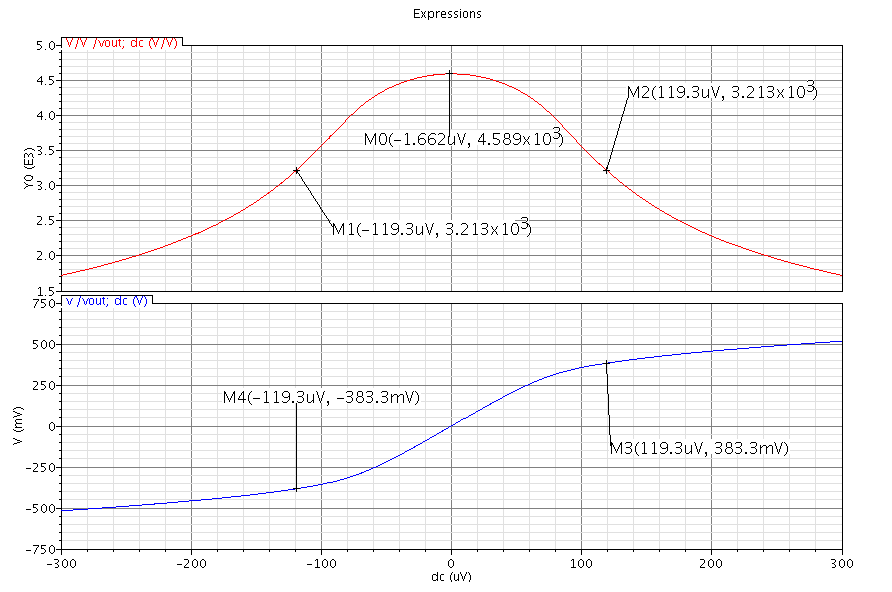
\includegraphics[width=\textwidth]{OTAoutputswing}
\caption{DC Output Swing Results} 
\label{fig:otaoutputswing}
\end{figure}
The peak open-loop gain is 4590. A reduction of 30\% of this value is a gain of 3213. The output voltage values at which the gain reaches 3213 are \SI{-383.3}{\milli\volt} and \SI{383.3}{\milli\volt}. This results in a total output swing of \SI{766.6}{\milli\volt}. This value is below the targeted output swing of \SI{1}{\volt}. An output swing of this value allows for approximately \nicefrac{1}{4} LSB of comparator offset. It was decided that with careful comparator design this tighter constraint could be met, so the output swing was deemed acceptable.
\subsection{OTA Noise}
Figure \ref{fig:otanoise} shows the results from the OTA AC noise simulations.
\begin{figure}[htbp]
\centering
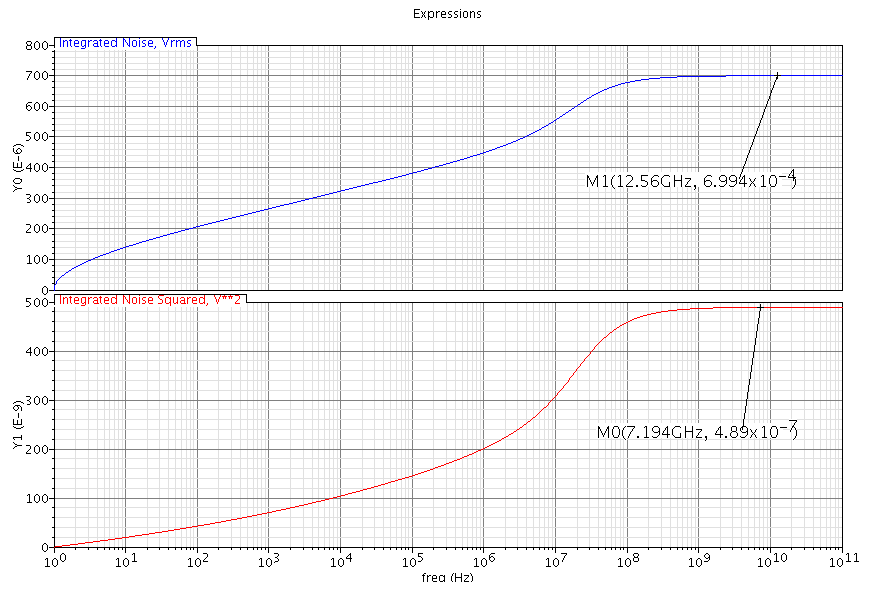
\includegraphics[width=\textwidth]{OTAnoise}
\caption{AC Noise Results} 
\label{fig:otanoise}
\end{figure}
The measured OTA output noise of \SI{699}{\micro\volt_{rms}} is still well below the maximum \SI{1.5}{\milli\volt_{rms}} allowed for in Table \ref{tab:maxoutputnoise}. This value is, however, well above the expected value calculated from \ref{eq:cascoutputnoise}. This is likely because the additional common-gate transistor causes much larger noise voltage on the output than allowed for by this equation. A better estimate would include the effects of the additional cascode stage and the additional gain it contributes to the common-source noise contribution. This calculation was not updated since the output noise was well within its limits.
\subsection{Real CMFB Transient Simulation}
In order to validate the operation of the passive CMFB network, a transiet simulation was performed. This transient simulation applied a sinusoidal input to the OTA and the output common-mode voltage was observed. Figure \ref{fig:cmfbresult} shows the output common-mode voltage measurements.
\begin{figure}[htbp]
\centering
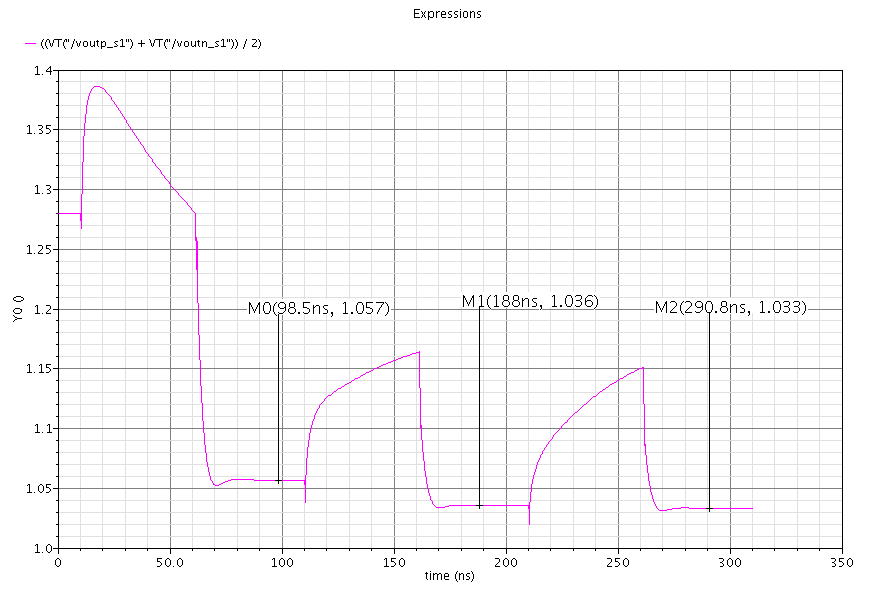
\includegraphics[width=\textwidth]{OTAcmfb}
\caption{Output Common-Mode Voltage Transient Simulation Results} 
\label{fig:cmfbresult}
\end{figure}
The deviations from the desired common-mode voltage observed occur during the $\phi_{1}$ clock phase and are the reason the OTA can only be active in the $\phi_{2}$ phase. While the OTA is in its active phase, the output common-mode agrees well with the desired common-mode voltage of \SI{1}{\volt}.
\subsection{Summary of OTA Simulation Results}
The measurements presented here show that the OTA achieved the performance desired for the ADC to achieve its performance specifications. Table \ref{tab:finalotadesign} summarizes the important design parameters, as well as the simulation results. Note that an additional transistor parameters had to be added to represent the PMOS load with different \gmid. Note also that $I_{total}$ is the total current used by the OTA, including additional current for the biasing circuits.
\begin{table}[htbp]
\begin{center}
\begin{tabular}{|l|r|}
\hline
Parameter & Value \\ \hline
$g_{m}/I_{d}$ & \SI{20}{\per\volt} \\ \hline
$(g_{m}/I_{d})_{PMOS,load}$ & \SI{15}{\per\volt} \\ \hline
$g_{m}$ & \SI{4.8}{\milli\siemens} \\ \hline
$I_{d}$ & \SI{694}{\micro\ampere} \\ \hline
$W_{PMOS}$ & \SI{280.7}{\micro\meter} \\ \hline
$W_{PMOS,load}$ & \SI{81.5}{\micro\meter} \\ \hline
$W_{NMOS}$ & \SI{92.5}{\micro\meter} \\ \hline
Loop gain & \SI{54.7}{\decibel} \\ \hline
$f_{c}$ & \SI{23.7}{\mega\hertz} \\ \hline
Phase Margin & \SI{89.3}{\degree} \\ \hline
Power & \SI{1.25}{\milli\watt} \\ \hline
Noise & \SI{699}{\micro\volt_{rms}} \\ \hline
\end{tabular}
\caption{Final OTA Design Parameters and Results}
\label{tab:finalotadesign}
\end{center}
\end{table}
\section{ADC Simulation Results With Integrated OTA}
Once the OTA performance was deemed acceptable, the next step was to perform the simulations outlined in Section \ref{sec:adcsimulations} on the differential ADC design with the transistor-level OTA model in place of the ideal OTA model. This section provides a summary of these results.

The first check for the ADC was a transient settling test. Since the performance of the OTA directly impacts the settling performance of the output to the second stage, ensuring that this test met its requirements was a very important step in verifying the OTA integration. Figures \ref{fig:tranotapos} and \ref{fig:tranotaneg} show the results from the transient simulation.
\begin{figure}[htbp]
\centering
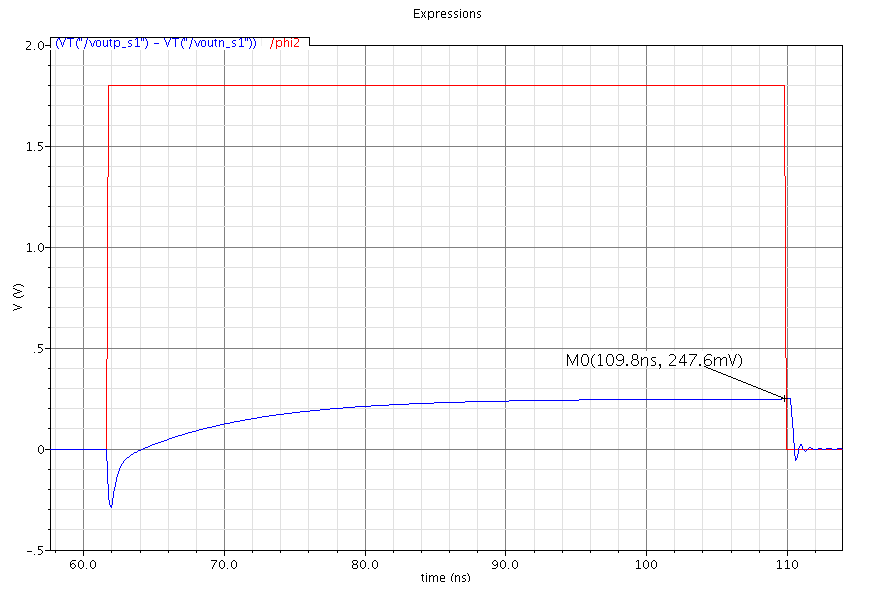
\includegraphics[width=\textwidth]{SAR_settlingfullpos}
\caption{Transient Settling of ADC With Real OTA Design With Full-Scale Positive Input Voltage} 
\label{fig:tranotapos}
\end{figure}
\begin{figure}[htbp]
\centering
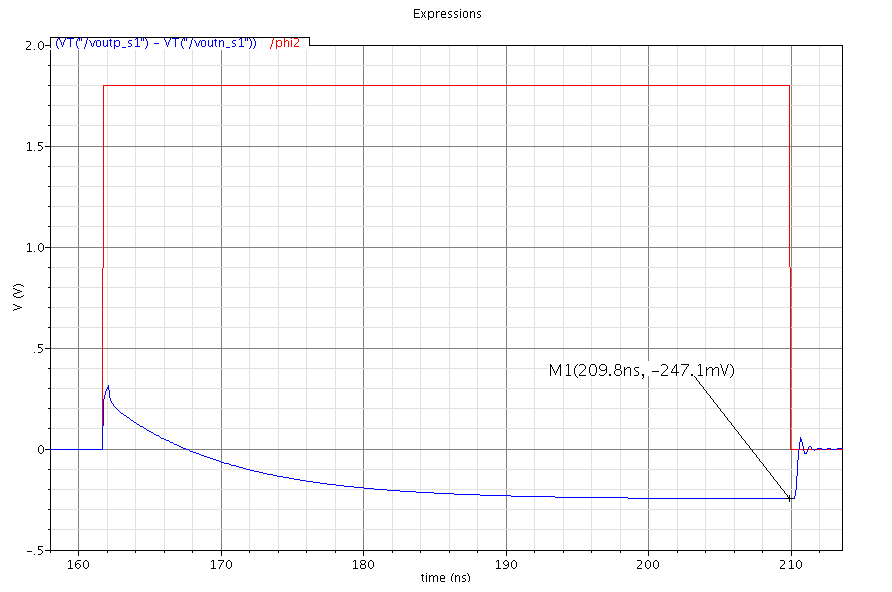
\includegraphics[width=\textwidth]{SAR_settlingfullneg}
\caption{Transient Settling of ADC With Real OTA Design With Full-Scale Negative Input Voltage} 
\label{fig:tranotaneg}
\end{figure}
In the case of the positive input, the settling error is \SI{-2.4}{\milli\volt}. In the case of the negative input, the transient settling error is \SI{2.9}{\milli\volt}. In both of these cases, the settling error is within the maximum settling error envelope.

Next, the full DFT simulation could be performed to measure the SQDR of the ADC. Figure \ref{fig:realotasqdr} shows the results from this simulation. 
\begin{figure}[htbp]
\centering
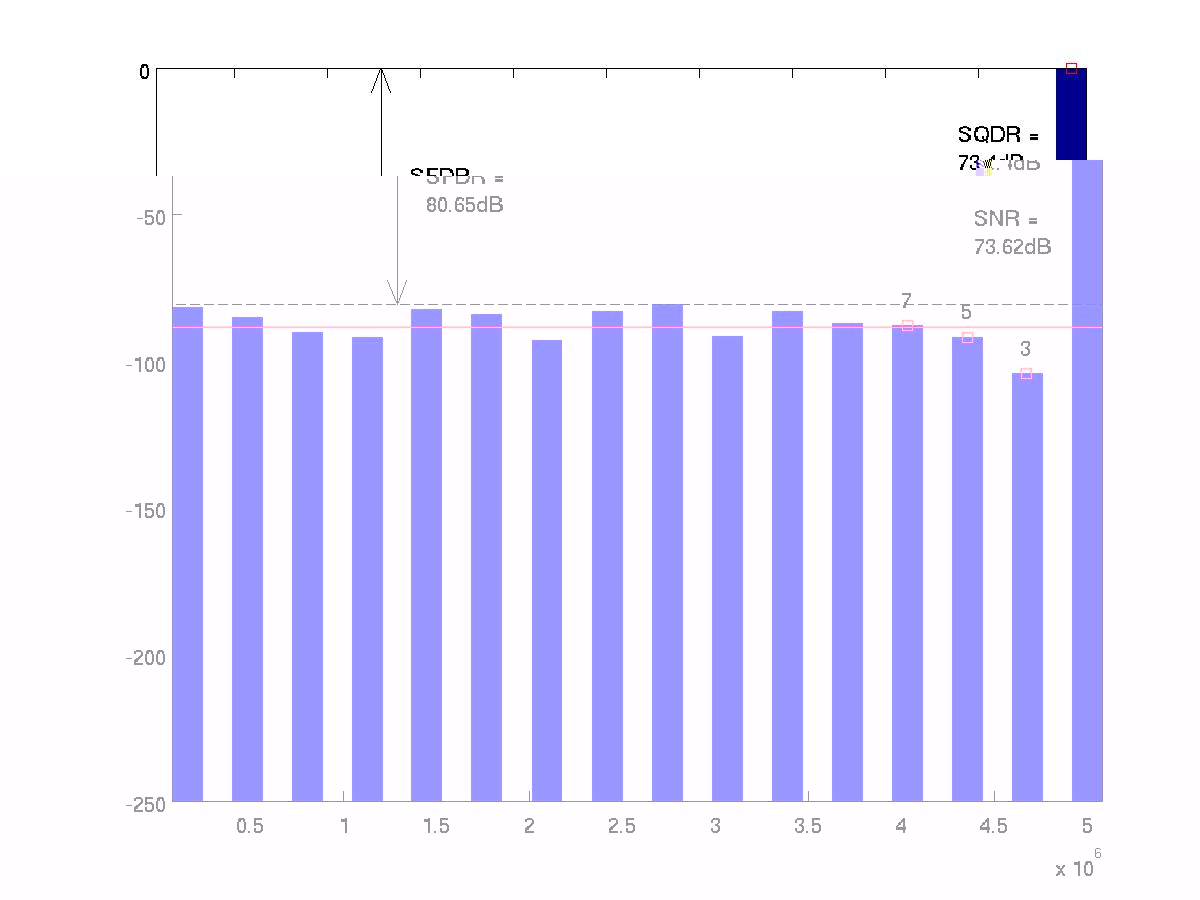
\includegraphics[width=\textwidth]{real_ota_diff_two_stage_douttotal_fft}
\caption{DFT of ADC With Real OTA Design } 
\label{fig:realotasqdr}
\end{figure}
The obtained SQDR was \SI{73.4}{\decibel}, a slight degradation from the ideal simulations. This degradation is expected, however, since simulations involving real transistors will have additional non-linearities that are not present in the ideal model. In addition, the SQDR is still very close to the ideal 12-bit SQDR, so this result was considered acceptable.

After performing the SQDR simulations, the noise performance of the entire ADC could be simulated. Only the AC noise in the hold phase and the PNOISE simulations needed to be rerun. Since the OTA is not active in the sampling phase, the OTA does not contribute to the output noise in that phase. Figure \ref{fig:otaholdnoise} is a graph of the simulated ADC noise in the hold phase.
\begin{figure}[htbp]
\centering
\includegraphics[width=\textwidth]{OTAholdnoise}
\caption{AC Noise During Hold Phase of ADC With Real OTA } 
\label{fig:otaholdnoise}
\end{figure}
The total output noise during the hold phase is \SI{723}{\micro\volt_{rms}}, which is in good agreement with the simulations performed only on the OTA model. The additional output noise is likely contributed from the switches. Once again, the output noise in the hold phase is well within budget. Table \ref{tab:acnoisesummaryrealota} summarizes the results from the AC noise simulation.
\begin{table}[htbp]
\begin{center}
\begin{tabularx}{\linewidth}{|l|X|X|X|X|}
\hline
Setup & AC Sampling Noise (\si{\milli\volt_{rms}}) & Total AC Hold Noise  (\si{\milli\volt_{rms}}) & AC Total Noise  (\si{\milli\volt_{rms}}) \\ \hline
Simulation & 1.52 & 0.72 & 1.68 \\ \hline
Calculation & 1.51 & 0.34 & 1.55 \\ \hline
Design Target & 1.51 & 1.52 & 2.15 \\ \hline
Error (\%) & 0.22 & 114.19 & 8.36 \\ \hline
Headroom (\%) & -0.22 & 52.52 & 21.75 \\ \hline
\end{tabularx}
\caption{AC Noise Summary With Real OTA}
\label{tab:acnoisesummaryrealota}
\end{center}
\end{table}

After obtaining AC noise simulations that were within budget, the PNOISE simulation was run to ensure good agreement between AC noise and PNOISE simulations. The graph from the PNOISE simulation is shown in Figure \ref{fig:pnoiserealota}
\begin{figure}[htbp]
\centering
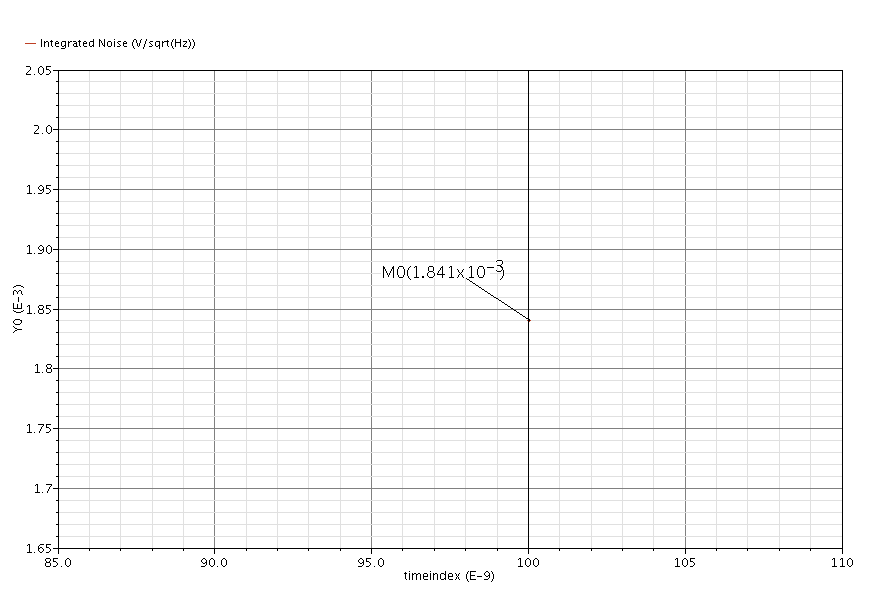
\includegraphics[width=\textwidth]{SAR_realota_pnoise}
\caption{PNOISE Simulation Results of ADC With Real OTA } 
\label{fig:pnoiserealota}
\end{figure}
While the PNOISE results are higher than that obtained from the AC noise simulations, the results are still within 20\% of each other. This level of agreement was considered acceptable for the noise simulations. Table \ref{tab:pnoisesummaryrealota} compares the results of the PNOISE simulation with the calculated values as well as the obtained AC noise measurements.
\begin{table}[htbp]
\begin{center}
\begin{tabularx}{\linewidth}{|l|X|X|X|}
\hline
Differential Noise &  &  &  \\ \hline
Setup & Total Noise Power (\si{\milli\volt_{rms}}) & Error vs Calculation (\%) & Error vs AC Simulation (\%) \\ \hline
PNOISE Simulations & \multicolumn{1}{r|}{1.84} & \multicolumn{1}{r|}{18.75} & \multicolumn{1}{r|}{9.58} \\ \hline
\end{tabularx}
\caption{ADC With Real OTA PNOISE Output Noise Summary}
\label{tab:pnoisesummaryrealota}
\end{center}
\end{table}

After obtaining acceptable results frm the noise simulation, the power consumption of the design could be simulated. Table \ref{tab:powerconsumptionrealota} summarizes the simulated average total current consumption and the contribution to the total from different circuit blocks.
\begin{table}[htbp]
\begin{center}
\begin{tabular}{|l|l|l|}
\hline
Circuit Block & Current (\si{\micro\ampere}) & Percent of Total \\ \hline
OTA & \SI{694}{\micro\ampere} & {80.98} \\ \hline
Digital logic and SAR capacitors & \SI{163}{\micro\ampere} & {19.02} \\ \hline
Total & \SI{857}{\micro\ampere} &  \\ \hline
\end{tabular}
\end{center}
\caption{ADC Power Consumption Summary}
\label{tab:powerconsumptionrealota}
\end{table}
From this average current, the average power consumption was calculated to be \SI{1.54}{\milli\watt}. 

As in the case of previous simulations, the results from the SQDR and noise simulations could be combined to obtain an SNDR and ENOB. Additionally, the ENOB, sampling frequency, and power consumption numbers could be combined to obtain the final FOM of the design. Since the PNOISE simulation produced the highest output noise, its value was used for the SNDR calculation. The SNDR calculated using these parameters was:
\begin{equation}
\label{eq:sndrdiffrealota}
SNDR = \SI{71.4}{\decibel}
\end{equation}
From Equation \ref{eq:sndridealdiff}, the ENOB is calculated to be 11.56 bits, which is still very close to an ideal 12-bit ADC performance.  Using Equation \ref{eq:fom}, the FOM for this design was calculated to be:
\begin{align}
\label{eq:fomrealota}
FOM &= \dfrac{\SI{1.54}{\milli\watt}}{\SI{10}{\mega\hertz}\cdot 2^{11.56}} \\[0.5em]
	&= 51\dfrac{\si{\femto\joule}}{\textnormal{conv-step}}
\end{align}
This number compares favorably with that obtained in other SAR-based pipeline designs~\cite{murmannadcsurvey}.


\chapter{Conclusion}
This chapter summarizes the results and discusses future work for this design.
\section{Discussion}
This work presented the initial design stages of a SAR-based pipeline ADC. With ever increasing focus on portable applications, power efficiency in ADCs will only become more important in the future. SAR ADCs are well known to be power efficient for applications requiring low sampling rates and medium to high resolutions. Applying the principles of pipelined ADCs to a SAR topology can increase the SAR application space to medium speed applications while still maintaining the power efficiency and high accuracy of the SAR topology. This design used a half-gain MDAC topology in order to reduce the required output swing and to increase overall ADC linearity. The half-gain topology alowed for the use of a triple-cascode OTA, which ended up being a low current solution. A novel scheme to obtain an additional bit of accuracy without increasing capacitance by utilizing the dummy LSB capacitor was also implemented. Although ideal clocks, comparators, and switches were used the OTA performance generally dominates the power and SNDR figures. The total figure of merit obtained from this design show that this topology has a lot of promise for power constrained designs.
\section{Future Work}
While this design covers the majority of the implementation of the ADC, there is still much to be done to ensure that this design would perform adequately when taped out. Some additional architectural modifications could reduce the load capacitance of the design signficantly. In addition, there are circuit level optimizations that could be performed on both the OTA and the digital control logic. Finally, some additional blocks need to be designed and additional simulations need to be performed. 

An extension of the implementation scheme in \ref{sec:dummylsbarch} could be used to obtain an additional bit of accuracy, or alternatively to halve the load capacitance in the second stage. Additionally, the differential scheme produces an additional bit of resolution that is currently not being utilized. This could lead to a factor of four reduction in load capacitance from the second stage capacitors. This could result in reduced power consumption or an increased sampling rate. These facts, along with realistic data on the parasitics from the OTA, suggest some re-architecting of the design could be done. The resolution of the two stages can be adjusted in order to achieve the best balance between sampling rate, power consumption, and total resolution. Furthermore, one large issue with the OTA design is that it will not scale well to future lower voltage processes. A reevaluation of the OTA topology used would like be a worthwhile exercise as well. Performing these architectural modifications could greatly improve the total performance of the design.

One disadvantage to the usage of the implementation scheme in \ref{sec:dummylsbarch} is the additional reference voltages required to obtain the additional bit of accuracy from the dummy LSB capacitor. The voltages used in this report were ideal, so the additional reference voltages did not affect the overall power consumption of the design. This would not be true in a real design, however. Designing additional voltage references that are at least 12-bit accurate is a non-trivial task and the implementation may end up consuming too much power to be beneficial for the design. An alternative scheme that introduces some imbalance in the SAR common-mode voltage can be used to obtain the additional bit without introducing more reference voltages. This scheme could only be implemented in the second stage of the pipeline, because introducing this imbalance could cause inaccuracies in the residue voltage. This is not a severe disadvantage, however, since the second stage sampling capacitance has a larger effect on the OTA power consumption than the first stage capacitance. Adding an additional bit to the first stage through traditional means would mean an increase in total area, but since the unit capacitance of the first stage is not at its minimum this increase could be mitigated slightly. This is a limitation that could likely be overcome. 

In addition to the architectural modifications the OTA and digital control logic performance could likely be improved at the circuit level. The OTA performance could likely be improved by reducing the input capacitance to the amplifier. Another area worth taking a second look at is the digital control logic. Although the OTA dominates total power consumption, the switching of the SAR capacitors and the digital control logic contribute about 20\% of the power. The digital logic was designed at the gate level using standard cells. It may be worthwhile to transform this design into register-transfer level (RTL) code, such as Verilog. Once this transformation is complete, a synthesis tool could be used to try to reduce the power consumption of the digital control logic even further. 

After completing this front-end work, the clocking network, comparators, and switches will need to be designed. Simulations will need to be run on all these blocks both individually and integrated into the ADC to ensure that the ADC will meet its performance requirements across all process corners. Once all this work is done, a layout and parasitic extraction can be performed. With this data, additional simulations and design adjustments can be performed in order to obtain a high level of confidence that a manufactured design will meet its specifications. Finally, the design will need to be manufactured and tested. Depending on the results from this testing, additional debugging and design adjustments may be necessary to achieve the desired performance. In the ideal case, first silicon would yield the desired results, but if this is not the case another manufacturing run could be performed with an additional round of testing to follow. If all goes well in this second stage, working silicon could be demonstrated.

%%%%%%%%%%%%%%%%%%%%%%%%%%%%%%%%%%%%%%%%%%%%%%%%%%%%%%%%%%%%%%%%%%%%%%
% Appendix/Appendices                                                %
%%%%%%%%%%%%%%%%%%%%%%%%%%%%%%%%%%%%%%%%%%%%%%%%%%%%%%%%%%%%%%%%%%%%%%
%
% If you have only one appendix, use the command \appendix instead
% of \appendices.
%
%\appendices
%\index{Appendices@\emph{Appendices}}%

%\chapter{Lerma's Appendix}
\index{Appendix!Lerma's Appendix@\emph{Lerma's Appendix}}%
The source \LaTeX{} file for this document is no longer quoted in
its entirety in the output document. A \LaTeX{} file can 
include its own source by using the command
\cn{verbatiminput\{\cn{jobname}\}}.





%%%%%%%%%%%%%%%%%%%%%%%%%%%%%%%%%%%%%%%%%%%%%%%%%%%%%%%%%%%%%%%%%%%%%%
% Generate the bibliography.					     %
%%%%%%%%%%%%%%%%%%%%%%%%%%%%%%%%%%%%%%%%%%%%%%%%%%%%%%%%%%%%%%%%%%%%%%
%								     %
% NOTE: For master's theses and reports, NOTHING is permitted to     %
%	come between the bibliography and the vita. The command      %
%	to generate the index (if used) MUST be moved to before      %
%	this section.						     %
%								     %
%\nocite{*}      % This command causses all items in the 		     %
                % bibliographic database to be added to 	     %
                % the bibliography, even if they are not 	     %
                % explicitly cited in the text. 		     %
		%						     %
\bibliographystyle{plain}  % Here the bibliography 		     %
\bibliography{diss}        % is inserted.			     %
%\index{Bibliography@\emph{Bibliography}}%			     %
%%%%%%%%%%%%%%%%%%%%%%%%%%%%%%%%%%%%%%%%%%%%%%%%%%%%%%%%%%%%%%%%%%%%%%
%%%%%%%%%%%%%%%%%%%%%%%%%%%%%%%%%%%%%%%%%%%%%%%%%%%%%%%%%%%%%%%%%%%%%%
% Vita page.							     %
%%%%%%%%%%%%%%%%%%%%%%%%%%%%%%%%%%%%%%%%%%%%%%%%%%%%%%%%%%%%%%%%%%%%%%

%\begin{vita}
%\end{vita}

%%%%%%%%%%%%%%%%%%%%%%%%%%%%%%%%%%%%%%%%%%%%%%%%%%%%%%%%%%%%%%%%%%%%%%
% Generate the index.						     %
%%%%%%%%%%%%%%%%%%%%%%%%%%%%%%%%%%%%%%%%%%%%%%%%%%%%%%%%%%%%%%%%%%%%%%
%								     %
% NOTE: For master's theses and reports, NOTHING is permitted to     %
%	come between the bibliography and the vita. This section     %
%	to generate the index (if used) MUST be moved to before      %
%	the bibliography section.				     %
%								     %
%\printindex%    % Include the index here. Comment out this line      %
%		% with a percent sign if you do not want an index.   %
%%%%%%%%%%%%%%%%%%%%%%%%%%%%%%%%%%%%%%%%%%%%%%%%%%%%%%%%%%%%%%%%%%%%%%



\end{document}
